\documentclass[letter,11pt]{book}
\usepackage[in]{fullpage}
\usepackage[utf8]{inputenc}
\usepackage[portuges]{babel}
\usepackage{graphicx}
\usepackage[]{natbib}
\usepackage{setspace}
\usepackage{pdfpages}
\usepackage[toc,page,title,titletoc]{appendix}
\usepackage[colorlinks={false},a4paper={true}]{hyperref}
\usepackage{url}
%\usepackage{listings}
\usepackage{fancyvrb}
\usepackage[small,bf,up]{caption}
\usepackage{subfigure}
\usepackage{natbib}
\usepackage{multirow}
\usepackage{courier}
\usepackage{rotating}

\onehalfspacing

\renewcommand{\appendixtocname}{Apendices}
\renewcommand{\appendixname}{Apendices}

\newcommand{\Backslash}[1]{\texttt{\symbol{92}}#1}

%\lstset{numbers=left,numberstyle=\tiny}
%\lstset{morecomment=[s][\color{blue}]{[u}{]\$}}
%\lstset{stringstyle=\ttfamily}
%\lstset{firstnumber=last}
%\lstset{basicstyle=\small}

\author{Diego Mauricio Ria\~{n}o Pach\'{o}n}
\title{Introdução a Bioinformática - CEN0485}


\begin{document}

\maketitle
\tableofcontents
\listoffigures

\chapter{Bases de bioinformática}


A bioinformática é uma disciplina que surge da interação entre biologia, estatística e ciência da computação. (Figura~\ref{bioinf}. Seus principais objetivos são a gestão e análise de grandes volumes de dados, principalmente o produto de novas tecnologias em biologia molecular, como genômica, proteômica e metabolômica, especialmente hoje com o advento de novas tecnologias de sequenciamento de ácidos nucleicos que estão revolucionando a forma como estudamos os genomas. Outro aspecto importante inclui o desenvolvimento de novos métodos computacionais, algoritmos e/ou softwares para a análise desses dados. 

De acordo com Philip Bourne (UCSD), ``a bioinformática tornou-se a intérprete da linguagem genômica do DNA e está tentando decifrar linguagens mais complexas em que as proteínas são os substantivos, as interações são a sintaxe, as vias metabólicas são frases e os sistemas vivos são o volume completo'' \citep{Bourne2004}.

Portanto, semelhante à biologia molecular, a bioinformática hoje constitui uma caixa de ferramentas que todo pesquisador de biologia tem que lidar \citetext{\citealp{Stein2008} apresenta um ponto de vista muito interessante}.

\begin{figure}[h]
\centering
   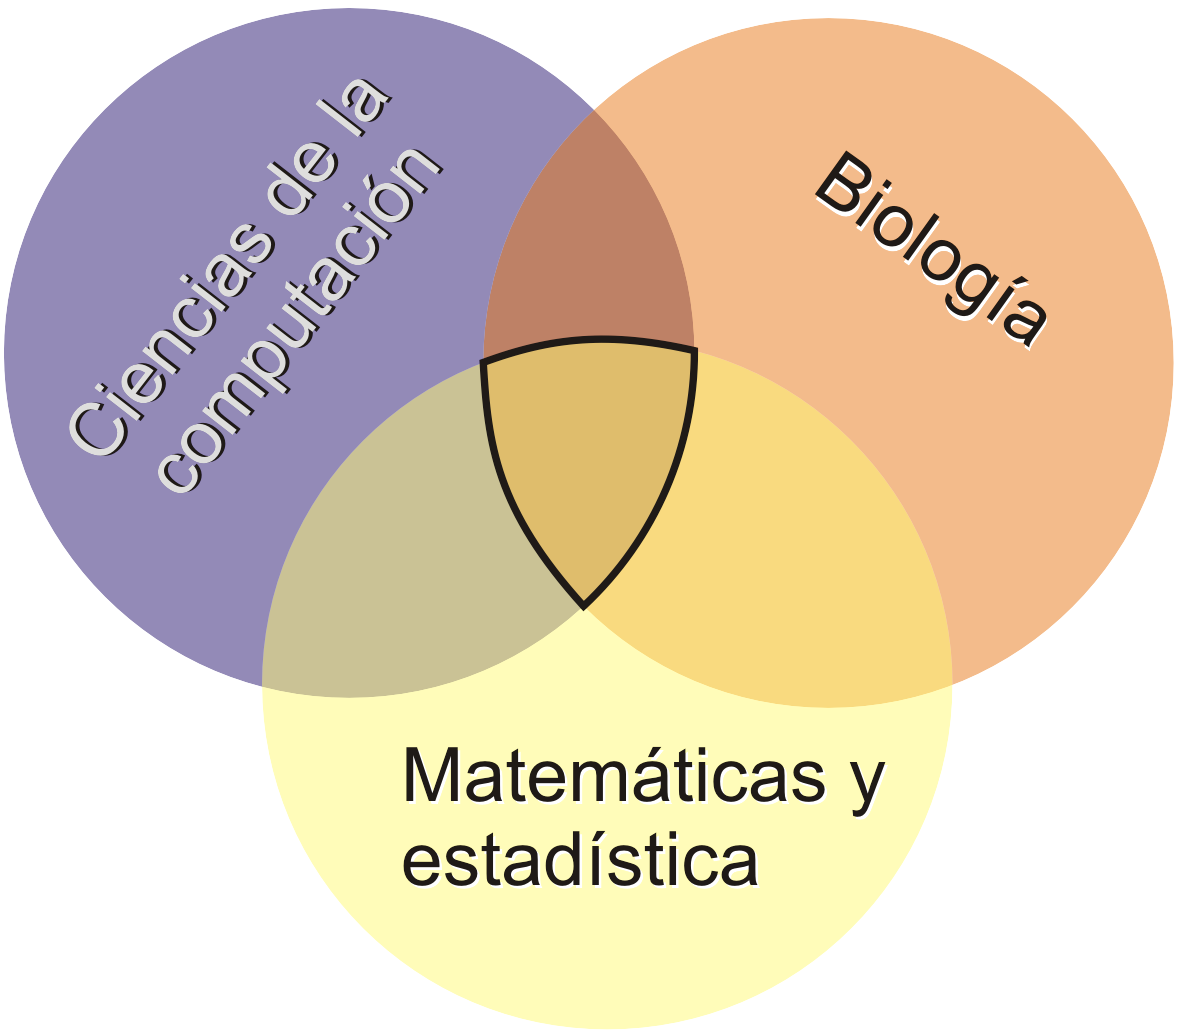
\includegraphics[height=5cm]{Figs/Bioinformatica.png}
  \caption[O que é bioinformática?]{\label{bioinf} A bioinformática é a disciplina que surge da interação de três ciências básicas: Biologia, Matemática e Ciência da Computação. Quando alguns deles dominam o resto, outra disciplina diferente da bioinformática é obtida, por exemplo, se matemática e biologia são mais importantes, obtemos biomatemáticos. É importante que as três ciências-base sejam equilibradas para realizar projetos de bioinformática.}
\end{figure}

Neste curso nos concentraremos na análise de dados biológicos, utilizando, na maioria dos casos, ferramentas de livre acesso, a maioria das quais têm melhor desempenho em sistemas operacionais Unix\footnote{Linux, MacOSX, BSD, etc. Se você quiser tentar ter uma cópia em sua home ou escritório de qualquer um desses sistemas operacionais, recomendo que você use o VirtualBox (ou outra tecnologia de virtualização), para instalar, por exemplo, o Linux dentro do sistema operacional existente, por exemplo, o Windows XP; Claro que é se você tem um camputador com pelo menos dois Núcleos e 2GB de RAM, caso contrário é mais conveniente ter um sistema dual boot.}.

\chapter{Ferramentas Unix úteis em bioinformática}
\section{Introdução ao sistema Unix}

O sistema operativo\footnote{Mais informações em \url{http://en.wikipedia.org/wiki/Operating_system}} é o conjunto de programas (``software'') que serve como uma interface entre a máquina ('hardware') e o usuário, e que permite que este último execute aplicativos. Os sistemas operacionais mais comuns são: Windows (XP, Vista), Unix e MacOS X. Sistemas operacionais semelhantes ao Unix (por exemplo, Linux) são usados principalmente em servidores, mas seu uso em estações de trabalho e desktops está em ascensão.  As principais características do Unix são: multitarefas, multi-usuário e portabilidade\footnote{Refere-se a quais programas criados em diferentes Unixes podem ser executados em um ou outro geralmente sem problemas.}. A maioria dos Unixes hoje tem uma interface gráfica fácil de usar, a partir da qual você pode realizar quase todas as tarefas de uso diário, como criar documentos, imprimir e navegar na Internet. Além dessa interface gráfica, há uma interface de linha de comando que permite ao usuário executar tarefas muito mais complexas e poderosas. Em seguida, aprenderemos como usar a linha de comando e alguns comandos que facilitam o manuseio de arquivos grandes, usando o Linux como sistema operacional. orientação sobre o uso de vários desses comandos está disponível no apêndice~\ref{unixguide}\footnote{Guias para outros programas comumente usados em bioinformática estão disponíveis em \url{http://www.embnet.org/en/QuickGuides}}.

\subsection{A linha de comando}

A linha de comando é acessada através de um programa de interpretação chamado ``shell''\footnote{\url{http://en.wikipedia.org/wiki/Unix_shell}}.  Existem vários tipos de ``shell'' em Unix. Na maioria das distribuições Linux o ``shell'' bash é instalado por padrão. Para usar o ``shell'' ou linha de comando do seu computador, inicie o programa \textbf{Terminal}, que tem um ícone semelhante ao mostrado na Figura~\ref{terminalico}.

\begin{figure}[ht]
\centering
   
\includegraphics[width=3cm]{Figs/terminalico.png}
  \caption{\label{terminalico}Ícone do programa da terminal}
\end{figure}

Clicando (uma ou duas vezes, dependendo da configuração) iniciará o programa \textbf{Terminal}, semelhante ao mostrado na Figura~\ref{terminal}. Este aplicativo da acesso à linha de comando Linux através de um \textit{prompt}, que informa que o sistema está esperando suas instruções. Na Figura~\ref{terminal}, o \textit{prompt} consiste na string \Verb+[user@server]$+, que consiste no nome do usuário que está usando o programa \textbf{Terminal}, seguido pelo nome da máquina e pelo símbolo do dólar, imediatamente após tem um cursor piscando esperando por seus comandos.

\begin{figure}[ht]
\centering
   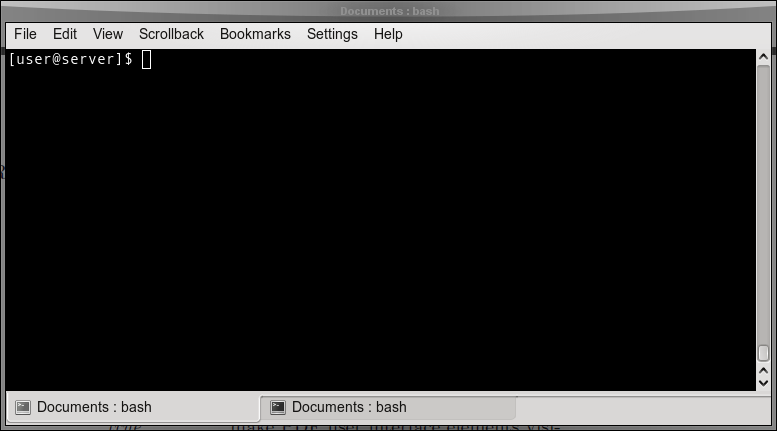
\includegraphics[width=10cm]{Figs/terminal.png}
  \caption{\label{terminal}Terminal no Linux}
\end{figure}

O \textit{prompt} pode ser modificado alterando a variável do sistema \Verb+PS1+\footnote{\url{http://tldp.org/HOWTO/Bash-Prompt-HOWTO/c141.html}}. Vamos alterar o \textit{prompt} para ter certeza de que todos temos o mesmo.

Na sessão  \textbf{Terminal} execute os comandos conforme mostrado na lista \textit{Alterando prompt}. Na linha~\ref{saveprompt} salvamos O prompt na nova variável \Verb+SAVE+, caso precisemos recuperá-lo. Na linha \ref{changeprompt} modificamos o \textit{prompt} atual, \Verb+\u+\footnote{Lista de modificadores de \textit{prompt} no bash: \url{http://tldp.org/HOWTO/Bash-Prompt-HOWTO/bash-prompt-escape-sequences.html}}, indica a nossa ``shell'' mostrar o usuario atual, \Verb+\h+, mostra o nome da  máquina e \Verb+\w+, mostra o diretório atual, o resto de caracteres são exibidos sem qualquer modificação\footnote{Exercício opcional: {\textquestiondown}Como tornar permanente a alteração de \textit{prompt}?}. Compare seu novo \textit{prompt} (línea~\ref{describeprompt}) com o antiguo (línea~\ref{promptini}), o símbolo \Verb+~+ refere-se ao diretório da sua home ou ao diretório do usuário, no sistema  (vea Sección~\ref{homedir})

\begin{Verbatim}[commandchars=!\{\},numbers=left,label=Alterando o prompt,frame=topline,fontsize=\scriptsize]
!textcolor{red}{[user@server]$} !label{promptini}
!textcolor{red}{[user@server]$} echo $PS1 !label{printprompt}
[\u@\h]$
!textcolor{red}{[user@server]$} SAVE=$PS1 !label{saveprompt}
!textcolor{red}{[user@server]$} PS1="[\u@\h:\w]$ " !label{changeprompt}
!textcolor{red}{[user@server:~]$} !label{describeprompt}
\end{Verbatim} 

Vamos começar interagir com o sistema através de comandos. para começar a executar o comando mostrado na linha~\ref{wgetini}, \Verb+wget+ é um programa para baixar arquivos da rede. A linha \ref{wgetinistart} ate \ref{wgetinistop} mostram a saida tipica deste comando, pode mudar levemente do que se amostra no seu \textbf{Terminal}. quando este comando termina executar o mostrado na linha~\ref{tarini}, que abre o arquivo que você acabou de baixar.

\begin{Verbatim}[commandchars=!\{\},numbers=left,firstnumber=last,label=Baixando arquivos, frame=topline,fontsize=\scriptsize]
!textcolor{red}{[user@server:~]$} wget https://github.com/labbces/cen0485/raw/main/linux/practicas/file1.tar.gz !label{wgetini}
--2022-03-25 16:26:12--  https://github.com/labbces/cen0485/raw/main/linux/practicas/file1.tar.gz !label{wgetinistart}
Resolving github.com (github.com)... 20.201.28.151
Connecting to github.com (github.com)|20.201.28.151|:443... connected.
HTTP request sent, awaiting response... 302 Found
Location: https://raw.githubusercontent.com/labbces/cen0485/main/linux/practicas/file1.tar.gz [following]
--2022-03-25 16:26:18--  https://raw.githubusercontent.com/labbces/cen0485/main/linux/practicas/file1.tar.gz
Resolving raw.githubusercontent.com (raw.githubusercontent.com)... 185.199.108.133, 185.199.109.133, 185.199.111.133, ...
Connecting to raw.githubusercontent.com (raw.githubusercontent.com)|185.199.108.133|:443... connected.
HTTP request sent, awaiting response... 200 OK
Length: 73501 (72K) [application/octet-stream]
Saving to: ‘file1.tar.gz’

file1.tar.gz                                      100%[==========================================================================================================>]  71,78K   141KB/s    in 0,5s    

2022-03-25 16:26:19 (141 KB/s) - ‘file1.tar.gz’ saved [73501/73501] !label{wgetinistop}

!textcolor{red}{[user@server:~]$} tar xzf file1.tgz !label{tarini}
\end{Verbatim} 

\subsection{Sua home e árvore diretórios\label{homedir}}

Cada usuário em um sistema Unix tem um espaço reservado, geralmente dentro do diretório ``\Verb+/home+'', em um subdiretório que tem o mesmo nome do usuário, e.g., para o usuário ''diriano'' seu diretório pessoal é ``\Verb+/home/diriano+'', e é chamado de diretório ''home'' ou diretório de usuário.  A primeira vez que você faz login no Linux ou \textbf{Terminal}, está localizado em seu diretório home. se a qualquer momento você não sabe onde você está, você pode usar o comando mostrado na linha \ref{pwd} para localizar o caminho dentro da árvore do diretório em que está localizada. é importante que você note que diretórios usam o caracter ``\Verb+/+'' para se referir a um caminho subdiretório aninhado como mostrado na linha~\ref{currdir} no listado \textit{Navegando pela árvore de diretórios}.

A árvore diretório refere-se à organização aninhada de diretórios no sistema de arquivos (Figura~\ref{arboldir}), semelhante à organização de diretórios no Microsoft Windows\texttrademark que pode ser visto com o \textbf{Windows Explorer}.

\begin{figure}[ht]
\centering
   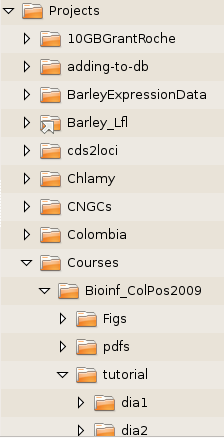
\includegraphics[width=4cm]{Figs/arboldir.png}
  \caption{\label{arboldir}Árvore de diretórios no Linux}
\end{figure}

Com o comando ``listar'' (Línea~\ref{ls}) exibe os diretórios e arquivos que estão no diretório atual. Este comando recebe argumentos/opções que permitem obter mais informações sobre arquivos e diretórios. Uma das opções mais utilizadas é `\Verb+-l+' (``menos ele''; Linha\ref{lsl}), cuja saída é exibida nas linhas \ref{lslout11} ate \ref{lslout22}, onde a lista de diretórios no local atual é exibida, juntamente com permissões nesses diretórios, o número de subdiretórios, tamanho, data da última modificação e nome.

\begin{Verbatim}[commandchars=!\{\},numbers=left,firstnumber=last,label=Navegando pela árvore de diretórios,frame=topline,fontsize=\scriptsize]
!textcolor{red}{[user@server:~]$} pwd !label{pwd}
/home/user !label{currdir}
!textcolor{red}{[user@server:~]$} ls  !label{ls}
dia1 dia2
!textcolor{red}{[user@server:~]$} ls -l  !label{lsl}
total 0  !label{lslout11}
drwxr-xr-x  2 user  group  68 Aug  5 09:01 dia1/
drwxr-xr-x  2 user  group  68 Aug  5 09:02 dia2/ !label{lslout22}
!textcolor{red}{[user@server:~/dia1]$} cd dia1 !label{cddia}
!textcolor{red}{[user@server:~]$} cd ..
!textcolor{red}{[user@server:~]$} cd /home/user/dia2/ !label{cdabsolutepath}
\end{Verbatim} 

Como mencionado acima, os sistemas Unix são multi-usuários, o que implica que deve haver um sistema de permissão no sistema de arquivos, para evitar perdas acidentais de dados, e.g., que um usuário delete dados de outro. Na linha~\ref{lslout2} as permissões de diretório são exibidas \Verb+dia2+ na primeira corda antes do primeiro espaço. O primeiro caractere indica se estamos em n diretório (\Verb+d+), um arquivo (\Verb+-+), ou um link (\Verb+l+). os 9 caracteres a seguir são divididos em 3 grupos de 3 caracteres cada, como mostrado na figura~\ref{permisos}\footnote{Exercício opcional: {\textquestiondown}Como alterar as permissões de um arquivo ou diretório?}.

\begin{figure}[ht]
\centering
   
\includegraphics[width=5cm]{Figs/permisos.png}
  \caption[Sistema de permissão no Linux]{\label{permisos}Sistema de permissão no Linux. r: permissão de leitura; w: permissão de escrita; x: permissão de Execução.}
\end{figure}

Já sabemos como exibir informações sobre diretórios e arquivos na localização atual. Para alterar o diretório usamos o comando `\Verb+cd nome_direitorio+', como se mostra na linha~\ref{cddia}. se você quiser subir um nível na hierarquia do diretório executar o comando \Verb+cd ..+, outra opção é usar o caminho absoluto do diretório que você quer alcançar, como mostrado na linha~\ref{cdabsolutepath}. Retornar ao subdiretório \Verb+/home/usuario/dia1+.

Antes de continuar, eu gostaria de introduzir o comando mais importante de qualquer sistema Unix, é o comando ``manual'', que mostra informações sobre o uso dos diferentes comandos, por favor, use-os sempre que você tiver alguma dúvida sobre as opções ou sintaxe de qualquer comando, e.g., \Verb+man ls+.

\subsection{Organizando arquivos}

As operações mais comuns com arquivos são: copiar, mover e excluir. A sintaxe dos comandos para mover ou copiar é a mesma: ``comando fonte destino''. Por exemplo, suponha que você tem um arquivo chamado ''test1.txt'' em seu diretório home e você quer movê-lo para o diretório``\Verb+~/dia1/+'', você teria que executar o comando mostrado na linha~\ref{movertest}. Você pode criar e remover diretórios (vazios) usando os comandos \Verb+mkdir+ y \Verb+rmdir+, respectivamente.

\begin{Verbatim}[commandchars=!\{\},numbers=left,firstnumber=last,label=Organizando aquivos e direitorios,frame=topline,fontsize=\scriptsize]
!textcolor{red}{[user@server:~]$} cd
!textcolor{red}{[user@server:~]$} ls -l
total 0  !label{lslout1}
drwxr-xr-x  2 user  group  68 Aug  5 09:01 dia1/
drwxr-xr-x  2 user  group  68 Aug  5 09:02 dia2/
!textcolor{red}{[user@server:~]$} touch test1.txt
!textcolor{red}{[user@server:~]$} ls -l
total 0  !label{lslout2}
drwxr-xr-x  2 user  group  68 Aug  5 09:01 dia1/
drwxr-xr-x  2 user  group  68 Aug  5 09:02 dia2/
-rw-r--r--  1 user  group   0 Aug 18 20:42 test1.txt
!textcolor{red}{[user@server:~]$} mv test1.txt dia1/ !label{movertest}
!textcolor{red}{[user@server:~]$} ls -l dia1/
total 0
-rw-r--r--  1 user  group  0 Aug 18 20:42 test1.txt
!textcolor{red}{[user@server:~]$} ls -l
drwxr-xr-x  2 user  group  68 Aug  5 09:01 dia1/
drwxr-xr-x  2 user  group  68 Aug  5 09:02 dia2/
!textcolor{red}{[user@server:~]$}
\end{Verbatim} 

\subsection{Algumas operações básicas com arquivos}
Usando alguns comandos UNIX podemos obter informações sobre arquivos, e as informações que eles contêm, de forma rápida e eficiente, muitas vezes não é necessário abrir o arquivo, que pode ter vários megabytes, para obter essas informações.

No subdiretório``\Verb+~/dia1/+'', encontra o arquivo ``TAIR9\_pep\_20090619'', que corresponde ao banco de dados de sequências proteicas previstas no genoma da planta modelo \textit{Arabidopsis thaliana}. para saber quantas linhas este arquivo tem execute o comando mostrado na linha~\ref{wc}.

Porque as diferenças nas saídas dos comandos executados nas linhas~\ref{wc}~e~\ref{wcl}\footnote{Revise a página do manual: \Verb+man wc+}?

Como mostrado na linha~\ref{tamanoarapep}, o tamanho deste banco de dados é de $18.173.159$ bytes. Para saber o quanto isso corresponde em uma unidade mais amigável use o comando mostrado na linha~\ref{lslh}.

Na maioria dos casos é importante ver como o arquivo é, seja no seu início ou no final, mas devido ao grande tamanho dos arquivos com os quais você normalmente trabalha, não é conveniente abrir o arquivo com qualquer editor de texto, pois isso poderia reduzir o tempo de resposta do computador. Os comandos exibidos nas linhas~\ref{head10}~y~\ref{tail10}, mostram a primeira e últimas 10 linhas no arquivo, respectivamente.

Usando o comando \Verb+grep+, como mostrado na linha~\ref{grepsimple}, você pode obter uma lista das linhas no arquivo de interesse que contêm um determinado padrão, i.e., uma sequência de texto específica.

\begin{Verbatim}[commandchars=!\{\},numbers=left,firstnumber=last,label=Operações básicas com arquivos,frame=topline,fontsize=\scriptsize]
!textcolor{red}{[user@server:~]$} cd dia1/
!textcolor{red}{[user@server:~/dia1]$} ls -l
total 35496
-rw-r--r--  1 user group  18173159 Aug 30 16:14 TAIR9_pep_20090619 !label{tamanoarapep}
-rw-r--r--  1 user group                0 Aug 18 20:42 test1.txt
!textcolor{red}{[user@server:~/dia1]$} wc TAIR9_pep_20090619 !label{wc}
  274243  790613 18173159 TAIR9_pep_20090619
!textcolor{red}{[user@server:~]$} wc -l TAIR9_pep_20090619 !label{wcl}
  274243 TAIR9_pep_20090619
!textcolor{red}{[user@server:~/dia1]$} ls -lh !label{lslh}
total 35496
-rw-r--r--  1 user group    17M Aug 30 16:14 TAIR9_pep_20090619
-rw-r--r--  1 user group       0B Aug 18 20:42 test1.txt
!textcolor{red}{[user@server:~/dia1]$} head TAIR9_pep_20090619 !label{head10}
>AT1G51370.2 | Symbols:  | F-box family protein
MVGGKKKTKICDKVSHEEDRISQLPEPLISEILFHLSTKDSVRTSALSTKWRYLWQSVPG
LDLDPYASSNTNTIVSFVESFFDSHRDSWIRKLRLDLGYHHDKYDLMSWIDAATTRRIQH
LDVHCFHDNKIPLSIYTCTTLVHLRLRWAVLTNPEFVSLPCLKIMHFENVSYPNETTLQK
LISGSPVLEELILFSTMYPKGNVLQLRSDTLKRLDINEFIDVVIYAPLLQCLRAKMYSTK
NFQIISSGFPAKLDIDFVNTGGRYQKKKVIEDILIDISRVRDLVISSNTWKEFFLYSKSR
PLLQFRYISHLNARFYISDLEMLPTLLESCPKLESLILVMSSFNPS*
>AT1G50920.1 | Symbols:  | GTP-binding protein-related
MVQYNFKRITVVPNGKEFVDIILSRTQRQTPTVVHKGYKINRLRQFYMRKVKYTQTNFHA
KLSAIIDEFPRLEQIHPFYGDLLHVLYNKDHYKLALGQVNTARNLISKISKDYVKLLKYG
!textcolor{red}{[user@server:~/dia1]$} tail TAIR9_pep_20090619 !label{tail10}
LLRYLTI*
>ATMG00070.1 | Symbols: NAD9 | NADH dehydrogenase subunit 9
MDNQFIFKYSWETLPKKWVKKMERSEHGNRSDTNTDYLFQLLCFLKLHTYTRVQVSIDIC
GVDHPSRKRRFEVVYNLLSTRYNSRIRVQTSADEVTRISPVVSLFPSAGRWEREVWDMFG
VSFINHPDLRRISTDYGFEGHPLRKDLPLSGYVQVRYDDPEKRVVSEPIEMTQEFRYFDF
ASPWEQRSDG*
>ATMG00130.1 | Symbols: ORF121A | hypothetical protein
MASKIRKVTNQNMRINSSLSKSSTFSTRLRITDSYLSSPSVTELAPLTLTTGDDFTVTLS
VTPTMNSLESQVICPRAYDCKERIPPNQHIVSLELTYHPASIEPTATGSPETRDPDPSAY
A*
!textcolor{red}{[user@server:~/dia1]$} grep ">" TAIR9_pep_20090619 | head -n 4  !label{grepsimple}
>AT1G51370.2 | Symbols:  | F-box family protein
>AT1G50920.1 | Symbols:  | GTP-binding protein-related
>AT1G36960.1 | Symbols:  | unknown protein
>AT1G44020.1 | Symbols:  | DC1 domain-containing protein
\end{Verbatim} 

Nem sempre na bioinformática lidamos com sequências, em muitos casos temos dados em forma tabular, onde os campos são separados por algum caractere definido, por exemplo, Guias ou vírgulas. Na maioria dos casos, isso envolve armazenar e gerenciar os dados usando um sistema de banco de dados, como o MySQL. No entanto, é importante ter uma ideia dos resultados antes de integrá-los ao sistema de banco de dados, uma opção que apareceu recentemente, voltada para biólogos que trabalham com grandes quantidades de dados, é o Scriptome\footnote{\url{http://sysbio.harvard.edu/csb/resources/computational/scriptome/UNIX/}}, em que o autor oferece uma coleção de scripts PERL que podem ser executados na linha de comando. Nas linhas~\ref{scriptomeexample1}~ate~\ref{scriptomeexample2} pode ver um exemplo onde todos os caracteres são alterados para maiúsdia, o comando tem que ser executado em uma única linha, aqui é mostrado em linhas separadas apenas para facilitar sua visualização.

\begin{Verbatim}[commandchars=!\{\},numbers=left,firstnumber=last,label=Exemplo do Scriptome,frame=topline,fontsize=\scriptsize]
!textcolor{red}{[user@server:~/dia1]$} perl -e ' while(<>) !{print lc($_);!} \  !label{scriptomeexample1}
warn "Changed $. lines to lower case\n" ' \
!textcolor{blue}{TAIR9_pep_20090619} > !textcolor{blue}{TAIR9_pep_20090619.lc}    !label{scriptomeexample2}
changed 274243 lines to lower case
!textcolor{red}{[user@server:~/dia1]$} ls -l
total 70992
-rw-r--r--  1 user  group  18173159 Aug 30 16:14 TAIR9_pep_20090619
-rw-r--r--  1 user  group  18173159 Aug 30 19:54 TAIR9_pep_20090619.lc
-rw-r--r--  1 user  group                0 Aug 18 20:42 test1.txt
!textcolor{red}{[user@server:~/dia1]$} head -n 2 TAIR9_pep_20090619.lc
>at1g51370.2 | symbols:  | f-box family protein
mvggkkktkicdkvsheedrisqlpepliseilfhlstkdsvrtsalstkwrylwqsvpg
!textcolor{red}{[user@server:~/dia1]$} 
\end{Verbatim} 

Na linha ~\ref{grepsimple} foi usado o símbolo ``\Verb+|+'' ou ``barra vertical'', ou ``pipe'' no UNIX, permite conectar comandos, de modo que a saída da esquerda da barra vertical sirva de entrada para o comando à direita da barra. Na linha~\ref{scriptomeexample2} foi usado o símbolo ``\Verb+>+'' para redirecionar a saída padrão do comando para um arquivo.

\section{Formatos de sequência\label{sequenceformats}}

Existem diferentes formatos para sequências, geralmente em texto simples. O que significa que eles podem ser vistos e editados com qualquer editor de texto, como \Verb+vi+ o \Verb+pico+. alguns desses formatos são mais comuns do que outros e muitos programas de bioinformática aceitam vários dos formatos mais comuns. \citep{Leonard2007}.

Todos os formatos de sequência têm uma característica (campo) em comum: um identificador para cada sequência. Para que possa ser reconhecido inequivocamente.

\subsection{Fasta}

O formato mais simples é conhecido como Fasta\footnote{\url{http://www.ncbi.nlm.nih.gov/blast/fasta.shtml}}. Em que uma entrada, sequência, pode ser dividida em duas partes: A linha de identificação, que \textbf{deve} começar com símbolo ``\Verb+>+'' e imediatamente seguido pelo identificador de sequência (Ver linha~\ref{fastaid}), qpode ser qualquer sequência de caracteres sem espaços. As linhas imediatamente após o identificador correspondem à sequência em si (Líneas~\ref{fastastartseq}-\ref{fastaendseq}).

Fasta é o formato de sequência mais usado em aplicações na bioinformática.
 
\begin{Verbatim}[commandchars=!\{\},numbers=left,firstnumber=last,label=Secuencia en formato FastA,frame=topline,fontsize=\scriptsize]
>gi|110742030|dbj|BAE98952.1| putative NAC domain protein [Arabidopsis thaliana] !label{fastaid}
MEDQVGFGFRPNDEELVGHYLRNKIEGNTSRDVEVAISEVNICSYDPWNLRFQSKYKSRDAMWYFFSRRE !label{fastastartseq}
NNKGNRQSRTTVSGKWKLTGESVEVKDQWGFCSEGFRGKIGHKRVLAFLDGRYPDKTKSDWVIHEFHYDL
LPEHQRTYVICRLEYKGDDADILSAYAIDPTPAFVPNMTSSAGSVVNQSRQRNSGSYNTYSEYDSANHGQ
QFNENSNIMQQQPLQGSFNPLLEYDFANHGGQWLSDYIDLQQQVPYLAPYENESEMIWKHVIEENFEFLV
DERTSMQQHYSDHRPKKPVSGVLPDDSSDTETGSMIFEDTSSSTDSVGSSDEPGHTRIDDIPSLNIIEPL
HNYKAQEQPKQQSKEKVISSQKSECEWKMAEDSIKIPPSTNTVKQSWIVLENAQWNYLKNMIIGVLLFIS
VISWIILVG !label{fastaendseq}
\end{Verbatim} 

\subsection{GenBank}

O formato GenBank\footnote{\url{http://www.ncbi.nlm.nih.gov/Sitemap/samplerecord.html}}\footnote{\url{ftp://ftp.ncbi.nih.gov/genbank/release.notes/gb172.release.notes}} é usado pelo ``National Center for Biotechnology Information'' (NCBI\footnote{\url{http://www.ncbi.nlm.nih.gov/}}), o maior repositório de sequências, tanto ácidos nucleicos quanto proteínas, em todo o mundo. O NCBI juntamente com o EMBL\footnote{\url{http://www.ebi.ac.uk/embl/}} e o DDBJ\footnote{\url{http://www.ddbj.nig.ac.jp/}},  manter em conjunto ``The International Nucleotide Sequence Database'' \citep{Mizrachi2008}.

Uma entrada neste formato é composta por duas partes. A primeira parte consiste em posições de 1 a 10, e geralmente contém o nome do campo, e.g., \Verb+LOCUS+, \Verb+DEFINITION+, \Verb+ACCESSION+ o \Verb+SOURCE+. A segunda parte de cada entrada contém as informações para o campo correspondente. Cada entrada termina com o símbolo ``\Verb+\\+'' (Linha~\ref{endgenbank}). Você pode encontrar mais informações sobre este tipo de arquivo seguindo o link \url{http://www.ncbi.nlm.nih.gov/Sitemap/samplerecord.html}


\begin{Verbatim}[commandchars=!\{\},numbers=left,firstnumber=last,label=Sequência em formato GenBank,frame=topline,fontsize=\tiny]
LOCUS       BAE98952                 429 aa            linear   PLN 27-JUL-2006
DEFINITION  putative NAC domain protein [Arabidopsis thaliana].
ACCESSION   BAE98952
VERSION     BAE98952.1  GI:110742030
DBSOURCE    accession AK226863.1
KEYWORDS    .
SOURCE      Arabidopsis thaliana (thale cress)
  ORGANISM  Arabidopsis thaliana
            Eukaryota; Viridiplantae; Streptophyta; Embryophyta; Tracheophyta;
            Spermatophyta; Magnoliophyta; eudicotyledons; core eudicotyledons;
            rosids; eurosids II; Brassicales; Brassicaceae; Arabidopsis.
REFERENCE   1
  AUTHORS   Totoki,Y., Seki,M., Ishida,J., Nakajima,M., Enju,A., Morosawa,T.,
            Kamiya,A., Narusaka,M., Shin-i,T., Nakagawa,M., Sakamoto,N.,
            Oishi,K., Kohara,Y., Kobayashi,M., Toyoda,A., Sakaki,Y.,
            Sakurai,T., Iida,K., Akiyama,K., Satou,M., Toyoda,T., Konagaya,A.,
            Carninci,P., Kawai,J., Hayashizaki,Y. and Shinozaki,K.
  TITLE     Large-scale analysis of RIKEN Arabidopsis full-length (RAFL) cDNAs
  JOURNAL   Unpublished
REFERENCE   2  (residues 1 to 429)
  AUTHORS   Totoki,Y., Seki,M., Ishida,J., Nakajima,M., Enju,A., Morosawa,T.,
            Kamiya,A., Narusaka,M., Shin-i,T., Nakagawa,M., Sakamoto,N.,
            Oishi,K., Kohara,Y., Kobayashi,M., Toyoda,A., Sakaki,Y.,
            Sakurai,T., Iida,K., Akiyama,K., Satou,M., Toyoda,T., Konagaya,A.,
            Carninci,P., Kawai,J., Hayashizaki,Y. and Shinozaki,K.
  TITLE     Direct Submission
  JOURNAL   Submitted (26-JUL-2006) Motoaki Seki, RIKEN Plant Science Center;
            1-7-22 Suehiro-cho, Tsurumi-ku, Yokohama, Kanagawa 230-0045, Japan
            (E-mail:mseki@psc.riken.jp, URL:http://rarge.gsc.riken.jp/,
            Tel:81-45-503-9625, Fax:81-45-503-9586)
COMMENT     An Arabidopsis full-length cDNA library was constructed essentially
            as reported previously (Seki et al. (1998) Plant J. 15:707-720;
            Seki et al. (2002) Science 296:141-145).
            This clone is in a modified pBluescript vector.
            Please visit our web site (http://rarge.gsc.riken.jp/) for further
            details.
FEATURES             Location/Qualifiers
     source          1..429
                     /organism="Arabidopsis thaliana"
                     /db_xref="taxon:3702"
                     /chromosome="1"
                     /clone="RAFL08-19-M04"
                     /ecotype="Columbia"
                     /note="common name: thale cress"
     Protein         1..429
                     /product="putative NAC domain protein"
     Region          5..137
                     /region_name="NAM"
                     /note="No apical meristem (NAM) protein; pfam02365"
                     /db_xref="CDD:111274"
     CDS             1..429
                     /gene="At1g01010"
                     /coded_by="AK226863.1:89..1378"
ORIGIN      
        1 medqvgfgfr pndeelvghy lrnkiegnts rdvevaisev nicsydpwnl rfqskyksrd
       61 amwyffsrre nnkgnrqsrt tvsgkwkltg esvevkdqwg fcsegfrgki ghkrvlafld
      121 grypdktksd wvihefhydl lpehqrtyvi crleykgdda dilsayaidp tpafvpnmts
      181 sagsvvnqsr qrnsgsynty seydsanhgq qfnensnimq qqplqgsfnp lleydfanhg
      241 gqwlsdyidl qqqvpylapy enesemiwkh vieenfeflv dertsmqqhy sdhrpkkpvs
      301 gvlpddssdt etgsmifedt ssstdsvgss depghtridd ipslniiepl hnykaqeqpk
      361 qqskekviss qksecewkma edsikippst ntvkqswivl enaqwnylkn miigvllfis
      421 viswiilvg
// !label{endgenbank}
\end{Verbatim} 

\subsection{Algumas operações básicas com sequências no formato Fasta}

Para o restante desta seção, e para a próxima, usaremos apenas sequências no formato Fasta. Por favor, verifique se as sequências de \textit{A. thaliana} no arquivo \Verb+TAIR9_pep_20090619+ estão neste formato. Você pode usar o comando ``\Verb+head nome_arquivo+'', ou o comando ``\Verb+less nome_arquivo+''\footnote{Para sair de \Verb+less+ pressione ``\Verb+q+''}.

Você já teve que contar o número de sequências ou alterar o identificador de sequência no formato Fasta? Se for uma dúzia de sequências, isso poderia facilmente ser feito em qualquer editor de texto, mas quando há milhares de sequências a opção do editor de texto deixa de ser viável. Felizmente, alguns comandos Unix nos permitem executar essas tarefas simples rapidamente.

Como viu na linha~\ref{grepsimple}, o comando ``\Verb+grep+'' poderia nos ajudar a contar o número de sequências em um arquivo Fasta. o interruptor ``\Verb+-c+'' conta o número de linhas contendo um determinado padrão em um arquivo, e podemos tirar proveito do fato de que em um arquivo Fasta o símbolo ``\Verb+>+'' aparece apenas uma vez para cada sequência como mostrado na linha~\ref{contarseqs}.

\begin{Verbatim}[commandchars=!\{\},numbers=left,firstnumber=last,label=Usando comandos Unix com arquivos Fasta,frame=topline,fontsize=\scriptsize]
!textcolor{red}{[user@server:~]$} cd ~/dia1/
!textcolor{red}{[user@server:~/dia1]$} ls -l
total 70992
-rw-r--r--  1 user  group  18173159 Aug 30 16:14 TAIR9_pep_20090619
-rw-r--r--  1 user  group  18173159 Aug 30 19:54 TAIR9_pep_20090619.lc
-rw-r--r--  1 user  group                0 Aug 18 20:42 test1.txt
!textcolor{red}{[user@server:~/dia1]$} grep -c ">" TAIR9_pep_20090619 !label{contarseqs}
33410
!textcolor{red}{[user@server:~/dia1]$} sed 's/>/>ATH_/' TAIR9_pep_20090619 > TAIR9_pep_20090619.mod !label{sedsp}
!textcolor{red}{[user@server:~/dia1]$} head TAIR9_pep_20090619.mod
>ATH_AT1G51370.2 | Symbols: 
MVGGKKKTKICDKVSHEEDRISQLPEPLISEILFHLSTKDSVRTSALSTKWRYLWQSVPG
LDLDPYASSNTNTIVSFVESFFDSHRDSWIRKLRLDLGYHHDKYDLMSWIDAATTRRIQH
!textcolor{red}{[user@server:~/dia1]$}
\end{Verbatim} 

Em outras ocasiões é importante modificar o identificador de cada sequência, de modo que inclua, por exemplo, uma abreviação que represente o nome da espécie a que a sequência pertence. Novamente Unix nos permite fazer essa mudança muito rapidamente usando o comando \Verb+sed+ como mostrado na linha~\ref{sedsp}.

\chapter{Buscas em banco de dados biológicos}

Este capítulo corresponde a uma versão modificada de um guia original da professora Silvia Restrepo

\section{NCBI – Bancos de dados e busca de informações}

O National Center for Biotechnology Information, NCBI pela sigla em inglês, é uma instituição pública dos Estados Unidos da América, que guarda todas as informações sobre os genomas de várias espécies, bem como o maior banco de dados público sobre sequências de DNA e proteínas. Sua página principal da rede está localizada no seguinte link:
\url{http://www.ncbi.nlm.nih.gov/}

Este site conecta todos os dados disponíveis em seus servidores (PubMed, TODOS os bancos de dados (Entrez), Blast, OMIM, Books, TaxBrowser, Structure), conforme mostrado na Figura \ref{screenshotNCBI}. Embora o Entrez esteja listado como um dos serviços, na realidade quase todos eles dependem diretamente do Entrez. Por exemplo, PubMed e Taxonomy estão intimamente ligados ao Entrez. 

\begin{figure}[ht]
\centering
   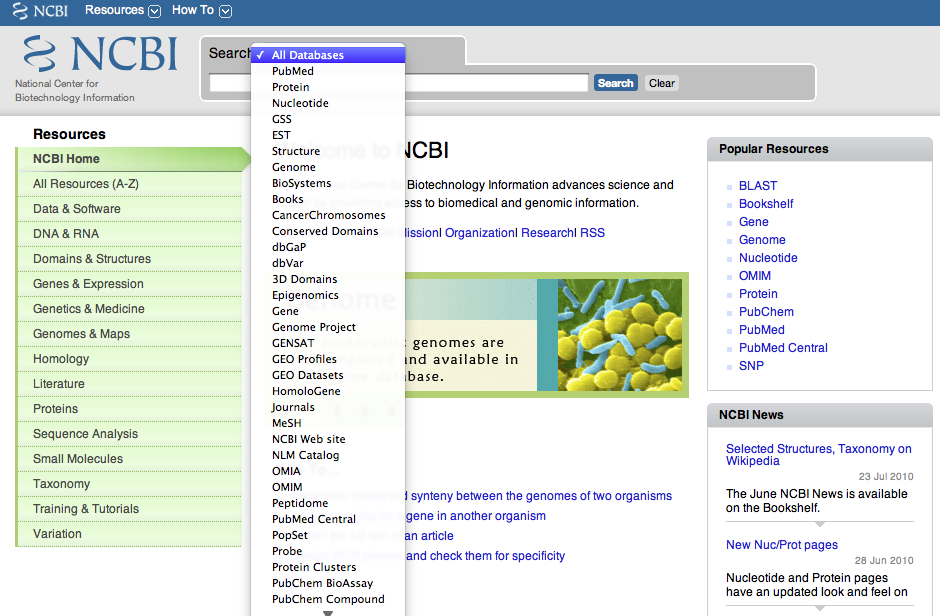
\includegraphics[width=15cm]{Figs/NCBIStart.png}
  \caption{\label{screenshotNCBI}Página inicial do NCBI}
\end{figure}

\subsection{Vamos começar uma visita aos seus bancos de dados}

Como primeiro passo, vamos entrar no PubMed. Esta base de dados contém informações sobre publicações científicas, e seus registros foram compilados pela NLM (National Library of Medicine), com a colaboração dos editores. Lá você encontrará a maioria das referências necessárias, incluindo o resumo (Abstract) e em alguns casos a publicação gratuita. 

Para obter ajuda sobre como realizar buscas consulte o seguinte link:  \url{http://www.ncbi.nlm.nih.gov/bookshelf/br.fcgi?book=helppubmed}

As páginas possuem um menu de banco de dados em uma barra superior, as pesquisas devem ser colocadas na janela mostrada na Figura \ref{screenshotsearchbox}.

\begin{figure}[ht]
\centering
   
\includegraphics[width=15cm]{Figs/NCBISearchBox.png}
  \caption{\label{screenshotsearchbox}Janela de busca do NCBI }
\end{figure}
 
Uma busca deve ter um formato semelhante a este:

\begin{quote}
``\textbf{palavrachave}''[field] \textbf{operador lógico}  ``\textbf{palavrachave}''[field] \ldots
\end{quote}

Onde \textbf{palavra chave} é a palavra utilizada para identificar um registro (record) de acordo com o campo (field) utilizado. Por exemplo, uma palavra chave pode ser "Silva" no campo "authors". \textbf{Operador lógico} é qualquer um destes operadores booleanos: AND, OR, NOT, BUT, etc. Ao substituir por suas próprias palavras-chave no formato acima, lembre-se de que os campos devem estar entre colchetes [ ], mas os operadores são independentes (sem os símbolos, "" ), além disso, as aspas na palavra chave são opcionais, mas cumprem a função de forçar uma busca com a palavra exata ao invés de serem flexíveis. 

Por exemplo, se eu quiser pesquisar todos os artigos de 1999 publicados por Silva et al na revista Science, eu uso o seguinte comando: "Silva"[AU] AND 1999[DP] AND "science"[TA]. Quanto mais informações forem inseridas na busca, mais restrita será a resposta (por exemplo, se eu incluir mais autores). 

Os campos mais comuns que podem ser solicitados no PubMed são os seguintes:

\begin{description}
\item[All Fields [ALL]]  Inclui todos os campos pesquisáveis do PubMed. No entanto, apenas os termos em que não houver correspondência encontrada em uma das tabelas ou índices de tradução por meio do processo de Mapeamento Automático de Termos serão pesquisados em Todos os Campos. PubMed ignora palavras irrelevantes de consultas de pesquisa.  
\item[Author Name [AU]] Vários limites no número de nomes de autores incluídos na citação MEDLINE existiram ao longo dos anos (consulte a política NLM sobre nomes de autores). MEDLINE não lista o nome completo. O formato para pesquisar o nome do autor é: sobrenome seguido de espaço e até as duas primeiras iniciais seguidas de espaço e abreviação do sufixo, se for o caso, tudo sem pontos ou vírgula após o sobrenome (por exemplo, fauci as ou o'brien jc jr). Iniciais e sufixos podem ser omitidos durante a pesquisa. O PubMed trunca automaticamente o nome de um autor para levar em conta as iniciais variadas, por exemplo, o'brien j [au] recuperará o'brien ja, o'brien jb, o'brien jc jr, bem como o'brien j. Para desativar esse truncamento automático, coloque o nome do autor entre aspas duplas e qualifique com [au] entre colchetes, por exemplo, "o'brien j" [au] para recuperar apenas o'brien j. 
\item[EC/RN Number [RN]] Número atribuído pela Enzyme Commission para designar uma enzima específica ou pelo Chemical Abstracts Service (CAS) para números de registro.  
\item[Entrez Date [EDAT]] Data em que a citação foi adicionada ao banco de dados PubMed. As citações são exibidas na ordem Entrez Date, que é o último a entrar, o primeiro a sair. As datas ou intervalos de datas devem ser inseridos usando o formato AAAA/MM/DD [edat], ex. 1998/04/06 [ed.] . O mês e o dia são opcionais (por exemplo, 1998 [edat] ou 1998/03 [edat]). Para inserir um intervalo de datas, insira dois pontos (:) entre cada data (por exemplo, 1996:1997 [edat] ou 1998/01:1998/04 [edat])
\item[Issue [IP]] O número do número da revista em que o artigo é publicado.  
\item[Journal Title [TA]] A abreviatura do título do periódico, nome completo do periódico ou número ISSN .
\item[Language [LA]] 
\item[Publication Date [DP]] A data em que o artigo foi publicado. As datas ou intervalos de datas devem ser pesquisados usando o formato AAAA/MM/DD [dp], ex. 1998/03/06 [dp] . O mês e o dia são opcionais (por exemplo, 1998 [dp] ou 1998/03 [dp]). Para inserir um intervalo de datas, insira dois pontos (:) entre cada data (por exemplo, 1996:1998 [dp] ou 1998/01:1998/04 [dp]). 
O nome de um produto químico discutido no artigo. Sinônimos para o Nome da Substância do Conceito Complementar serão mapeados automaticamente quando qualificados com [nm]. Este campo foi implementado em meados de 1980. Muitos nomes químicos são pesquisáveis como termos MeSH antes dessa data.
\item[Text Words [TW]] Inclui todas as palavras e números no título e resumo, e termos MeSH, subtítulos, nomes de substâncias químicas, nome pessoal como assunto e campo MEDLINE Secondary Source (SI). O campo Nome pessoal do assunto também pode ser pesquisado diretamente usando a tag do campo de pesquisa [ps], por exemplo, rouxinol f [ps]. 
\item[Title Words [TI]] Palavras e números incluídos no título de uma citação. 
\item[Title/Abstract Words [TIAB]] Palavras e números incluídos no título e resumo de uma citação.
\item[Unique Identifiers [UID]]
\item[Volume [VI]] O número do volume da revista em que um artigo é publicado. 
\end{description}

Agora vamos no site onde o ENTREZ está localizado. Para fazer isso, selecione TODOS OS BANCOS DE DADOS na janela do banco de dados na página principal. Entrez é um sistema de busca de sequências armazenadas em bancos de dados.
Consultas sofisticadas podem ser solicitadas para obter um conjunto de sequências de seu interesse, por exemplo, posso pedir para exibir todas as sequências genômicas de Arabidopsis que foram incluídas no banco de dados entre os anos 97' e 99' que também contêm anotação (em a tabela "features") nas regiões promotoras. A Figura \ref{screenshotentrez} mostra a página de login do servidor Entrez.

\begin{figure}[ht]
\centering
   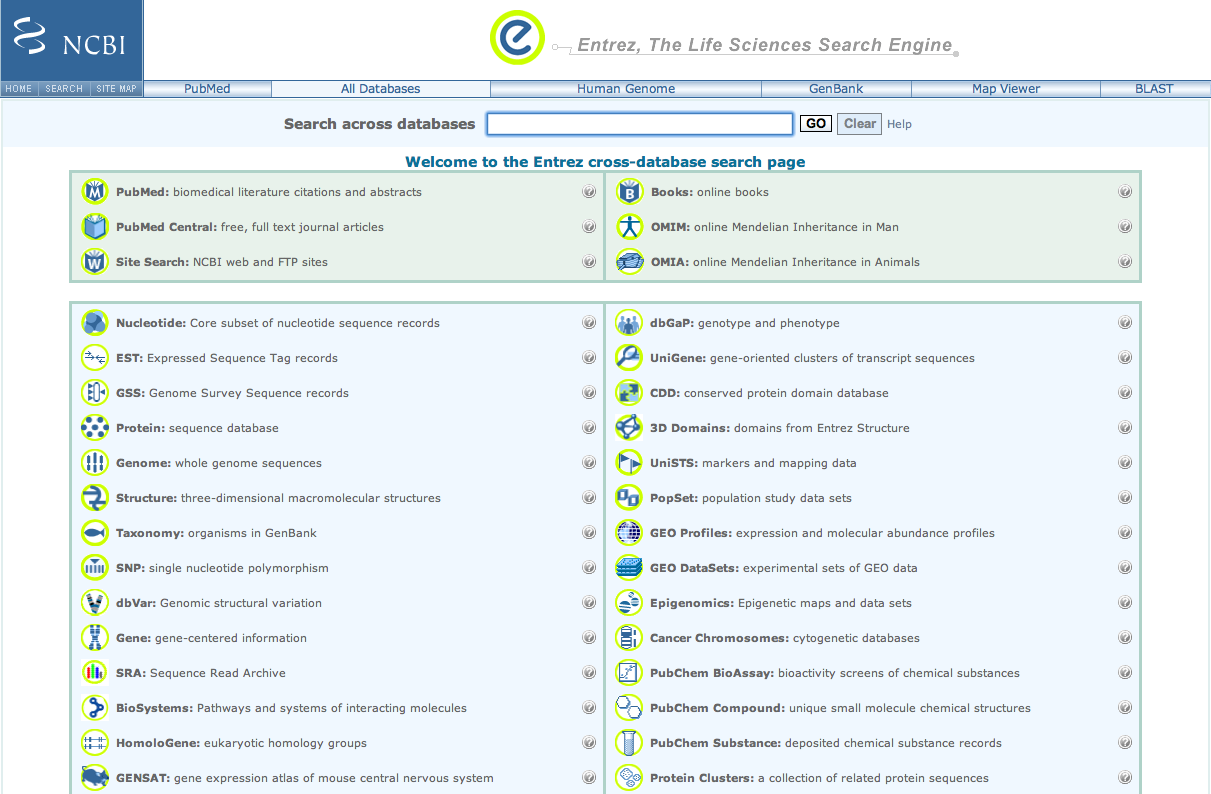
\includegraphics[width=15cm]{Figs/screenshotEntrez.png}
  \caption{\label{screenshotentrez}Página inicial do Entrez}
\end{figure}

Assim, em um único site podemos realizar buscas simultaneamente em todas as bases de dados ou selecionar uma única base de dados e realizar uma busca por base de dados. 

Na caixa de busca, as sequências podem ser consultadas usando seus números identificadores (como o gi-number ou com o número de acesso). Questões mais complicadas também podem ser formuladas usando a sintaxe entrez, semelhante a como vimos o PubMed: 

\begin{quote}
``\textbf{palavrachave}''[field] \textbf{operador lógico} ``\textbf{palavrachave}''[field] \ldots
\end{quote}

Para mais informações sobre o Entrez você pode seguir o link:
\url{http://www.ncbi.nlm.nih.gov/bookshelf/br.fcgi?book=helpentrez&part=EntrezHelp}

{\color{red}
\subsubsection{Exercícios}

\begin{enumerate}
\item Qual é a classificação taxonômica da alga \textit{Chlamydomonas reinhardtii}?, e quais outras plantas estão próximas, para que possam ser usadas como fonte de marcadores?. Quantas sequências de proteínas estão presentes no GenBank para a espécie \textit{Chlamydomonas reinhardtii}? 
\item Acesse a página do PubMed e obtenha as referências que tratam da biologia molecular e/ou genética da mandioca (\textit{Manihot esculenta}). Quantos foram publicados nos últimos dois anos e de quais laboratórios (ou regiões geográficas) são os autores? Explique como você pesquisou. Dica: GoPubMed \url{http://www.gopubmed.org/}
\item Use o Entrez para encontrar todas as sequências EST (Expressed Sequence Tag) de arroz que foram depositadas no banco de dados.
\end{enumerate}
}

Revise a descrição dos principais formatos de sequências na seção
\ref{sequenceformats}.

\subsubsection{Quais bancos de dados encontramos no NCBI?}

O NCBI possui um grande número de bancos de dados. O mais conhecido no GenBank que contém todas as sequências de nucleotídeos. GenPept contém as sequências de proteínas. Outras bases de dados são Genome, Structure, PubMed

No GenBank as sequências estão organizadas em 17 divisões, 11 tradicionais e 6 Bulk
Nas tradicionais, as sequências foram enviadas diretamente pelos pesquisadores, são caracterizadas e as divisões são:

\begin{description}
\item[PRI] primatas
\item[PLN] plantas
\item[BCT] bactérias
\item[INV] invertebrados
\item[ROD] Roedores
\item[VRL] Viral
\item[VRT] outros vertebrados
\item[MAM] Mamíferos (Ej. ROD + PRI)
\item[PHG] Fagos
\item[SYN] Sintético (vetores de clonagem, etc)
\item[UNA] sem anotação 
\end{description}


O Bulk consiste em sequências enviadas em grupos via email ou ftp, imprecisas e mal caracterizadas, são elas: 

\begin{description}
\item[dbEST] Banco de dados EST, tags de sequência expressa
\item[dbSTS] Sequence-tagged sites: são marcos genômicos curtos para os quais há informações de sequência e mapa. 
\item[dbGSS] Genomic survey sequences. Contém: dados de sequência do genoma de etapa única, sequências terminais BAC, YAC e cosmídeos, sequências de éxon
\item[dbHTGS] High-Throughput Genomic Sequences. Ele foi criado para salvar informações de sequenciamento de genoma que não foram finalizadas ou curadas, mas para torná-las conhecidas da comunidade científica assim que estiverem disponíveis.
\end{description}

e também existem bancos de dados para:

\begin{description}
\item[HTC] High Throughput cDNA
\item[PAT] Patent
\end{description}

\subsubsection{RefSeq}

Queremos colocar ênfase especial em um banco de dados NCBI chamado RefSeq. Este banco de dados foi criado para obter uma coleção biologicamente não redundante de sequências de DNA, RNA e proteínas. Cada RefSeq (sequência de referência) representa uma molécula única que ocorre naturalmente em um organismo. Esta base de dados é do tipo com curadoria de pesquisadores. Cada molécula não é um resultado de pesquisa, mas sim uma síntese de informações.

Vamos voltar para a página principal do NCBI e na janela de busca, deixando all databases, digite NC\_001139\footnote{certifique-se de incluir o símbolo de sublinhado}. Vemos que em Nucleotide temos 1 hit, assim como em Genome e em Gene temos 631.

Vamos abrir Nucleotide: obtemos um flatfile de sequência  que corresponde à sequência completa do cromossomo VII da levedura. Vamos dar uma olhada no arquivo flatfile, \textcolor{red}{quais informações ele contém?} 

Observemos que os identificadores desta base de dados mudam e são do tipo 2+6 com duas letras e 6 números, a tabela a seguir nos mostra o que significam essas letras: 

\begin{tabular}{|c|c|}
\hline  \multicolumn{2}{|l|}{\textbf{mRNA and Proteins}} \\
\hline  NM\_123456 & Curated mRNA  \\ 
\hline  NP\_123456 &  Curated Protein\\ 
\hline  NR\_123456 &  Curated non-coding RNA\\ 
\hline  XM\_123456 &  Predicted mRNA\\ 
\hline  XP\_123456 &  Predicted Protein\\ 
\hline  XR\_123456 &  Predicted non-coding RNA\\ 
\hline   \multicolumn{2}{|l|}{\textbf{Gene records}} \\
\hline  NG\_123456 & Genomic Region \\ 
\hline  \multicolumn{2}{|l|}{\textbf{Chromosome}} \\ 
\hline  NC\_123456 & Complete genomic molecule, Microbial replicons, organelle genomes  \\ 
\hline  \multicolumn{2}{|l|}{\textbf{Assemblies}} \\ 
\hline  NT\_123456 & Contig \\ 
\hline  NW\_123456 & WGS supercontig (assembly of WGS) \\ 
\hline 
\end{tabular} 

\subsection{Recuperação de Sequências no NCBI com buscas mais específicas}

\paragraph{CONHECEMOS O ORGANISMO.} As pesquisas do NCBI podem ser mais direcionadas se conhece o organismo sobre o qual estamos procurando informações. Entramos na página inicial do NCBI, vamos para TaxBrowser, colocamos o nome do organismo que estamos procurando. Ao selecioná-lo, uma tabela do número de sequências por tipo de molécula ou projeto aparece à direita. Clicar em uma delas, por exemplo proteínas, nos leva diretamente às proteínas daquele organismo. 

\paragraph{NÓS SABEMOS OS NÚMEROS DE ACESSO.} Se você souber o número de acesso diretamente, pode colocá-lo na janela de pesquisa da página principal do NCBI. Para várias sequências os números são colocados com a palavra OR entre eles, por exemplo AJ487842 ou AJ487843. Por fim, para uma sequência de números de acesso, digite: AJ487842::AJ487851[ACCN] 

\paragraph{DIRECIONAMOS A PESQUISA COM LIMITES.} Por exemplo, se eu quiser pesquisar as sequências de mRNA curadas relacionadas a um tipo de câncer em humanos, posso fazer a seguinte pesquisa: na janela de pesquisa, coloco COLON CANCER AND NONPOLYPOSIS , eu pesquiso o banco de dados de nucleotídeos. Então em LIMITS seleciono a molécula de mRNA e em only from (banco de dados) seleciono RefSeq. Então eu seleciono a outra janela Preview/index acima e lá em organismos eu escrevo humanos e seleciono AND 

\section{Recuperação de sequência usando SRS@EBI\label{srs}}

Existe no entanto uma excelente alternativa para a busca de sequências biológicas, que nos permite controlar quase todos os aspectos da nossa busca, esta alternativa é o Sequence Retrieval System (SRS). Este sistema foi desenvolvido com esta tarefa de recuperar eficazmente sequências biológicas em mente, daí o seu design e capacidades. 

Neste workshop trabalharemos com o SRS oferecido pelo European Bioinformatics Institute (EBI), \url{http://srs.ebi.ac.uk/}. Ou digitando EBI, (\url{http://www.ebi.ac.uk/}) , database~$\rightarrow$~database~browsing você chega ao SRS. 

Uma forma simples de consultar o SRS é através da caixa Quick Text Search. Nesta caixa é possível pesquisar em vários bancos de dados disponíveis no menu suspenso, conforme mostrado na Figura~\ref{screenshotSRS} 

\begin{figure}[ht]
\centering
   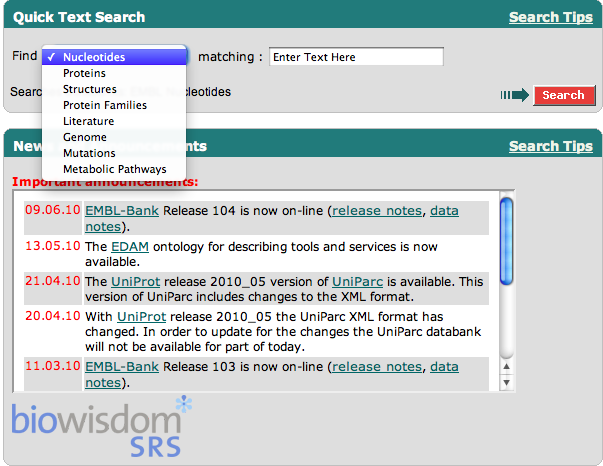
\includegraphics[width=15cm]{Figs/screenshorSRS.png}
  \caption{\label{screenshoteSRS}Página inicial do SRS}
\end{figure}

Por exemplo, selecionando a opção “Nucleotide Sequences”, realizaremos nossa busca no banco de dados EMBL DNA (homólogo ao genBank e DDBJ). 

Faça uma pesquisa rápida pelo HIV-1 com diferentes opções no menu suspenso. Até este ponto, o SRS parece ser um pouco menos completo em comparação com o site do NCBI, mas agora começaremos a ver onde está todo o seu potencial.

Agora vamos realizar uma busca avançada. Selecione a guia Library Page localizada na parte superior da tela e mostrada na Figura~\ref{optionsSRS} 

\begin{figure}[ht]
\centering
   
\includegraphics[width=15cm]{Figs/SRSMenu.png}
  \caption{\label{opcionesSRS}Opções SRS}
\end{figure}

Você será então levado para a seção SRS onde estão descritos cada um dos bancos de dados que compõem o sistema (Figura~\ref{SRSDBs}). Como você pode ver, o SRS inclui muitos bancos de dados ao mesmo tempo e essa é uma de suas principais virtudes, por isso o SRS às vezes é conhecido como "banco de dados de bancos de dados", pois através deste sistema podemos consultar vários bancos de dados ao mesmo tempo, de acordo com nossas necessidades particulares. 

\begin{figure}[ht]
\centering
   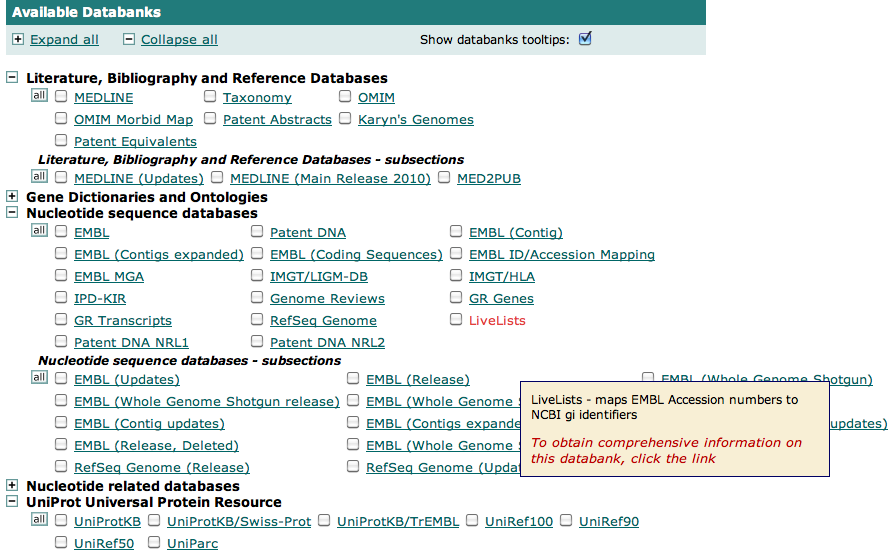
\includegraphics[width=12cm]{Figs/SRSDBs.png}
  \caption{\label{SRSDBs}Opções SRS}
\end{figure}

Como você pode ver, o SRS é semelhante ao sistema NCBI ENTREZ, no sentido de que nos permite consultar muitas bases de dados ao mesmo tempo, mas desta vez não se restringindo apenas àquelas que o NCBI possui, mas a praticamente qualquer base de dados. A quantidade de bancos de dados que o SRS possui depende de cada implementação, ou seja, o administrador do SRS determina quais bancos de dados deseja ou não incluir em seu sistema 

Posicione o cursor do mouse sobre qualquer uma das entradas, após alguns segundos aparecerá uma caixa de texto explicativa. \textcolor{red}{Que tipo de informação os bancos de dados EMBL (Contig Updates), UniprotKB/Swissprot fornecem?} 

Ao seguir o link para qualquer uma dessas bases de dados obteremos mais informações sobre ela, como o número de entradas presentes, data de atualização, etc. No entanto, por enquanto nosso interesse é selecionar algumas bases de dados para realizar nossas buscas. Marque as caixas para os bancos de dados ``UniprotKB/Swissprot'' e ``UniprotKB/TrEMBL''. Certifique-se de que esses sejam os únicos bancos de dados selecionados. 

À esquerda de sua tela você encontrará a caixa ``Search Options'' que nos permitirá selecionar o nível de profundidade de nossa busca. Como esta é a primeira vez que trabalhamos com este sistema, selecionaremos o formulário padrão de busca. 

Pressione o botão ``\textbf{Standard query Form}'' na caixa ``\textbf{Search Options}'' 

Esta ação o levará ao formulário de busca SRS padrão (Figura~\ref{searchform}).

\begin{description}
\item[Fields you can search] Campos de busca, onde podemos inserir nossos termos de busca de acordo com qualquer uma das opções presentes nos respectivos menus suspensos. 
\item[Create View] Criar vista, esta opção funciona em conjunto com a opção 3, e aqui podemos definir o tipo de campos que queremos ver na nossa página de resultados. Para o nosso exemplo, estamos interessados em selecionar todas as proteínas de superfície conhecidas de Plasmodium falciparum com atividade imunogênica, relacionadas ao merozoíto. 
\item[Result Display Options] Opções para exibir os resultados, onde podemos definir o número de resultados que queremos por página, bem como o formato de saída, seja um dos definidos no menu suspenso ou criando uma visualização personalizada (opção ``create view'').
\item[Search Options] Opções de busca, onde podemos definir, entre outras coisas, o tipo de conector lógico (Booleano) a ser usado para os termos definidos em 1. 
\end{description}


\begin{figure}[ht]
\centering
   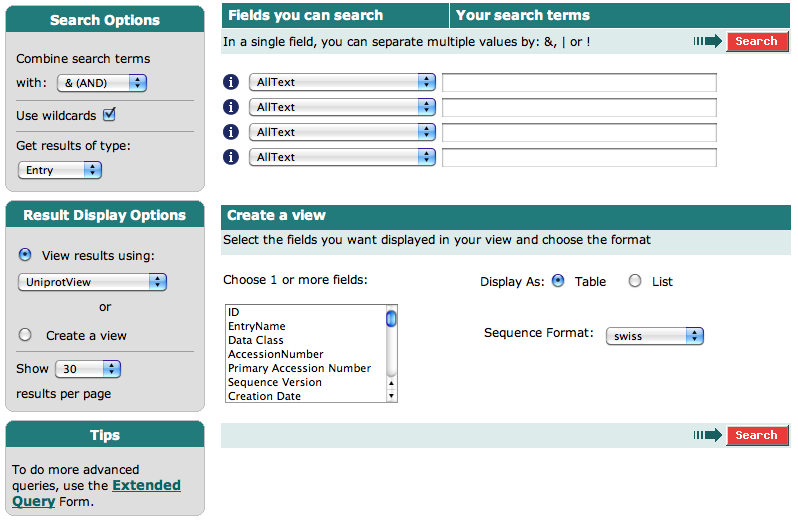
\includegraphics[width=12cm]{Figs/SearchFormSRS.png}
  \caption{\label{searchform}Formulário de pesquisa SRS}
\end{figure}

Defina estes critérios na seção ``Fields you can search'' de acordo com a  Figura~\ref{busquedaplasmodium}.

\begin{figure}[ht]
\centering
   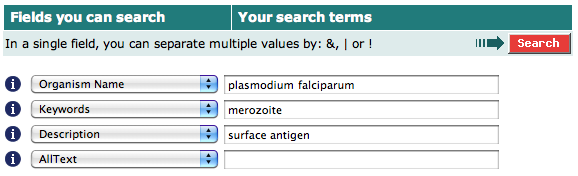
\includegraphics[width=10cm]{Figs/busquedaSRSplasmodium.png}
  \caption{\label{busquedaplasmodium}Critérios de pesquisa avançados}
\end{figure}

Em seguida, pressione o botão \textbf{``search''} localizado no topo desta seção e aguarde alguns segundos.

Com certeza você já tem uma visão mais exata das possibilidades oferecidas pelo SRS e suas principais diferenças com o sistema Entrez. Primeiro, conseguimos definir exatamente não apenas o banco de dados que queríamos consultar, mas as seções específicas dele. Além disso, também conseguimos definir exatamente os termos de pesquisa em seções específicas dos posts, o que nos dá total controle sobre os resultados que queremos obter. 

Brinque com as diferentes opções de formato que o SRS oferece na seção ``\textbf{Result Display Options}'' do formulário de pesquisa. Tente também criar seu próprio formato de saída com a opção ``\textbf{Create view}''. 

\textcolor{red}{Encontre todas as proteínas nucleares hipotéticas de \textit{Saccharomyces cerevisiae} e exiba a informação em formato fasta}. 

\chapter{Manipulación básica de secuencias}

Este capítulo corresponde a una versión modificada de una guía original de la profesora Silvia Restrepo.

\section{Limpieza de secuencias}

Un Vector, es un agente que lleva fragmentos de ADN de interés a una célula específica. Si éste es utilizado para reproducir un fragmento de ADN, se le conoce como \textit{Vector de Clonación}, si se utiliza para expresar cierto gen, se conoce como \textit{Vector de Expresión}. Los vectores más usados son plásmidos, BACs, YACs, cósmidos y los bacteriófagos Lambda y P1. En cualquier caso que se utilice un vector, cuando se manda a secuenciar el fragmento de interés, se puede identificar las secuencias vector y eliminarlas. Para esto se puede emplear VecScreen siguiendo el enlace \url{http://www.ncbi.nlm.nih.gov/VecScreen/} (Figura~\ref{screenshotVecScreen}).

\begin{figure}[ht]
\centering
   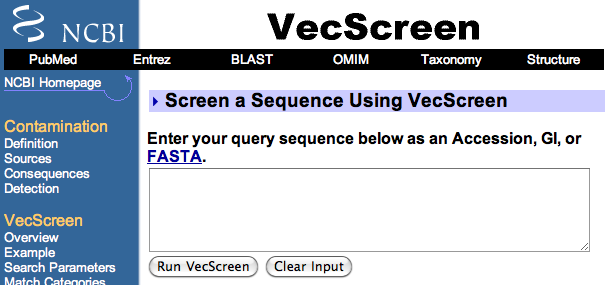
\includegraphics[width=10cm]{Figs/screenshotVecScreen.png}
  \caption{\label{screenshotVecScreen}VecScreen: Herramienta para detectar contaminación de vectores.}
\end{figure}

En el campo de búsqueda que aparece en la página, pegue la Secuencia Problema 1 y ejecútela como ``\textbf{Run VecScreen}''.

En la siguiente página, deje los campos que se encuentran por defecto (para ver los resultados de manera gráfica) y dele click a ``\textbf{View report}''.

Posibles resultados:

\begin{itemize}
\item Si la secuencia NO tiene secuencias de vector contaminantes: ``Non-significant homology''.
\item Si la secuencia SI tiene secuencias de vector contaminantes: 
 \begin{itemize}
 \item Sección gráfica: con diferentes colores muestra, sobre el mapa de la secuencia problema, donde se encuentran las secuencias contaminantes.
  \item Alineamiento: se muestra el alineamiento entre la secuencia problema y las secuencias contaminantes homólogas de vectores que se encontraron.
 \end{itemize}
\end{itemize}

\begin{Verbatim}[commandchars=!\{\},numbers=none,label=Secuencia problema 1,frame=topline,fontsize=\scriptsize]
>Secuencia_Problema_1 
TCTATNGGCGATTGGGTACCGGGCCCCCCCTCGAGGTCGACGGTATCGATAAGCTTGATA
TCGAATTCATGGGATTCTTAACAACAATAGTTGCTTGTTTCATTACCTTTGCAATATTAA
TTCACTCATCCAAAGCTCAAAACTCCCCCCAAGATTATCTTAACCCTCACAATGCAGCTC
GTAGACAAGTTGGTGTTGGCCCCATGACATGGGACAATAGGCTAGCAGCCTATGCCCAAA
ATTATGCCAATCAAAGAATTGGTGACTGCGGGATGATCCACTCTCATGGCCCTTACGGCG
AAAACCTAGCCGCCGCCTTCCCTCAACTTAACGCTGCTGGTGCTGTAAAAATGTGGGTCG
ATGAGAAGCGTTTCTATGATTACAATTCAAATTCTTGTGTAGGAGGAGTATGTGGACACT
ATACTCAGGTGGTGTGGCGTAACTCAGTACGTCTCGGTTGTGCTAGGGTTCGAAGCAACA
ATGGTTGGTTTTTCATAACTTGCAATTATGATCCACCAGGTAATTTTATAGGACAACGTC
CCTTTGGCGATCTTGAGGAGCAACCCTTTGATTCCAAATTGGAACTTCCAACTGATGTCT
AAGAATTCCTGCAGCCCGGGGGATCCACTAGTTCTAGAGCGGCCGCCACCGCGGTGGAGC
TCCAGCTTTTGTTCCCTTTAGTGAGGGTTAATTTCGAGCTTGGCGTAATCATGGTCATAG
CTGTTTCCTGTGTGAAATTGTTATCCGCTCACAATTCCACACAACATACGAGCCGGAAGC
ATAAAGTGTAAAGCCTGGGGTGCCTAATGAGTGAGCTAACTCACATTAATTGCGTTGCGC
TCACTGCCCGCTTTCCAGTCGGGAAACCTGTCGNGCCAGCTGCATTAATGAATCGGCCAA
CGCGCGGGGAAAAGGCGGGTTTGGCGTATTGGGGCGCTCTTCCGCTTCCTCGCTCACTGG
ACTCNGTTGCGCTCGGTCGTTCGGCTGCGGNGAGNGGNAATCAGCCNCCCCCCAAAAGGN
GGNNAATCCGGTTANCCNCGNAATCCGGGGGAAAACNCCNNGAAAAAACNTGGGGANCAA
AAAGGNCCCCAAAAAGGGCCCAGNAACCNNNNAAAAAGGGCCNGNGTTGNNNGGGGGTTT
TNCCAAAGGGNCCCCCCCCCCGNGAANANNNNCCAAAAANTCCCCCCCTCAATCCAANGG
GGNGAAAACCCCCCGGGNANTTTAAAAANANCGGGGGTTNCCCCNGGAAAACCCCCNGGG
NCNNCCNGGTTCCNACCCGGCCCTTAANGGAAAATGNCNCCNTTT
\end{Verbatim} 

{\color{red}
En la Secuencia Problema 1, ¿Encuentra fragmentos similares a algún vector?

En el caso en que encuentre secuencias contaminantes de vectores, ¿Entre qué nucleótidos se encuentra el inserto de interés?

Elimine las secuencias contaminantes y vuelva a VecSreen con esta nueva secuencia. ¿Qué obtiene?
}

Se debe entonces proceder a limpiar la secuencia eliminando los fragmentos correspondientes a vector. 

\section{Mapa de restricción}

Los mapas de restricción sirven para verificar que la secuencia que se recibió del centro de  secuenciación en efecto corresponde a la secuencia que se mando. Igualmente se puede usar esta herramienta para verificar largas secuencias (como genomas bacterianos) que fueron ensambladas a partir de fragmentos mas cortos. El número y tamaño de los fragmentos predichos deben corresponder al mapa de restricción experimental. 

Una herramienta que permite hacer este tipo de análisis se encuentra siguiendo el enlace \url{http://biotools.umassmed.edu}, seleccionando la opción ``Restriction Mapping Tool''. 

En la siguiente página pegue la secuencia ``35\_292648\_.ab1'' y seleccione la opción ‘entire linear map’ y ‘Submit Sequence to wwwtacg’. Note que tiene la opción de escoger que enzimas de restricción desea usar.

\begin{Verbatim}[commandchars=!\{\},numbers=none,label=Secuencia 35\_292648\_.ab1,frame=topline,fontsize=\scriptsize]
>35_292648_.ab1 ABIX Testing -- no comment RESTRICCION
CGGGCGTCACCGCATTTTTTTTTTTTTTTTTTTTTTTTTTTTTAAGGGATAATCTATTTC
NCTTATTCANANAATTAGTAATTACNCATAACNCNCAACTTTGANGCCCNCATTATAANG
ATTAGCAGGNCATTATATAAGNGGGCANCCTTTTATTTCANACATTAATTACTTAATTTN
GGGCAANCCANAAAANGGACAAGTCTAGAGTCNCATTACNGGGNACATATTTGCCTNGGG
TTCATCACTCTCNCCTTCACATACAAACTTTCCATCTTTACCAAAANAANAGCAACCCTT
GNACCCGGGGCAACANGGGGNACATCCGGGGGGANAAATTAACGATTTTCCTTGGGAACG
GGGACNTCTTGAANAGGCAATATTTGGATCNCAATTAANGGGGCAAGCNTTTGGCCTTTT
NGGATCANATTCNCCTTCNCAAATAAATTTTCCGAAAGAATTATAATAATTACNACCCTT
ATAGCCGGAGCAACAATTGANGCATANGGGATTTAGCGGACTTCCTTCTGAACGGGGGCA
TATCCCGAACCCAANATTACCNCATTCNCTAGTACAAGCCTNGGCATCAACATATAGAAA
CNTTCCAAGAACAATTAGTAGGNAAGCGACAAAATTAACTTCCTTGGGAACNGCCNNGAN
GGANAATTGATTACNAGTACCTNGGCTTCTTTTAATTTNGGGGNCGGGGGGGGGGGGGGG
\end{Verbatim}

La página de resultados le muestra la información de su secuencia, las enzimas que no cortan su secuencia, el número de cortes para cada enzima y un mapa de sus secuencias con los sitios de corte.

{\color{red}
¿La secuencia tiene sitios de corte para la enzima cfoI?

¿Si digiriera el fragmento con las enzimas EcoRI y BamH1 y corriera la digestión en un gel de agarosa, qué tamaños de bandas observaría?
}

\section{Análisis de la composición del ADN}

En esta sección vamos a usar algunos programas del paquete EMBOSS (``The European Molecular Biology Open Software Suite''; \url{http://emboss.sourceforge.net/}) para calcular algunas estadísticas sobre secuencias de ADN. Mas adelante nos volveremos a encontrar con EMBOSS para desarrollar tareas mas complicadas.

\subsection{Contenido de G$+$C}

El contenido en G$+$C de la secuencia de ADN es importante por varias razones. El apareamiento entre las bases G y C es más estable que entre las bases A y T. Así, el contenido en bases de la secuencia determinara el comportamiento de la secuencia en experimentos de laboratorio. 

Siguiendo el enlace \url{http://mobyle.pasteur.fr/cgi-bin/portal.py?form=geecee} llegará a una interfaz web del programa geecee del paquete EMBOSS, que le permite calcular el contenido de G$+$C de una secuencias de ADN.

\textcolor{red}{¿Cuál es el contenido de G$+$C de la secuencia 35\_292648\_.ab1?}

\subsection{Composición monomérica y palabras cortas}

También podemos fácilmente calcular las frecuencias de k-meros, i.e., monómeros, dímeros, trímeros, tetrámeros, pentámeros, \ldots

{\color{red}Siga el enlace \url{http://mobyle.pasteur.fr/cgi-bin/portal.py?form=compseq} y calcule la proporción de monómeros, dímeros y trímeros de la secuencia 35\_292648\_.ab1. Presente los resutados en forma tabular.}.

\chapter{Creación de bases de datos relacionales}

En este capítulo vamos a crear bases de datos relacionales usando SQLite\footnote{\url{http://www.sqlite.org/}\label{descargasqlite}} como motor de base de datos y la extensión de Firefox SQLite Manager\footnote{\url{https://addons.mozilla.org/en-US/firefox/addon/5817/}\label{sqllitemanager}} como interfaz a la base de datos.

Primero tenemos que asegurarnos que el programa \Verb+sqlite3+ está instalado en nuestro computador. Para esto iniciemos el programa \textbf{Terminal}\footnote{Como hacer esto depende del sistema operativo. En MacOSX puede usar spotlight, i.e., el ícono de lupa en la parte superior derecha de su escritorio, y escribir Terminal, luego darle click al ícono del programa.}. Una vez en \textbf{Terminal} podemos escribir \Verb+sqlite3+ en la línea de comandos, si se obtiene un salida similar a la mostrada en las líneas \ref{salidasqlite3ini} a \ref{salidasqlite3end}, \Verb+sqlite3+ está instalado y funcionando correctamente, de lo contrario es necesario descargarlo del sitio web referenciado en la nota al pie número \ref{descargasqlite}

\begin{Verbatim}[commandchars=!\{\},numbers=left,firstnumber=last,label=Ejecutando sqlite3,frame=topline,fontsize=\scriptsize]
!textcolor{red}{[user@server:~]$} sqlite3
SQLite version 3.6.12 !label{salidasqlite3ini}
Enter ".help" for instructions
Enter SQL statements terminated with a ";"
sqlite> !label{salidasqlite3end}
!textcolor{red}{[user@server:~]$} 
\end{Verbatim} 

Una vez hemos comprobado que el motor de bases de datos está instalado y funcionando correctamente, tenemos que asegurarnos que el complento \textbf{SQLite Manager} de \textbf{Firefox} esta instalaldo, para esto, en el \textbf{Firefox}, vaya al menú \textbf{Herramientas} $\to$ \textbf{SQLite Manager}; is esta opción de menú no aparece entonces es necesario instalar la interfaz a SQLite desde el sitio referenciado en la nota al pie número \ref{sqllitemanager}.

Una vez henmos comprobado que el \textbf{SQLite Manager} está instalado podemos hacer click en el menú \textbf{Herramientas} $\to$ \textbf{SQLite Manager}, lo que iniciará una ventana como la que se muestra en la figura \ref{sqlitemanagerrunning}

\begin{figure}[ht]
\centering
   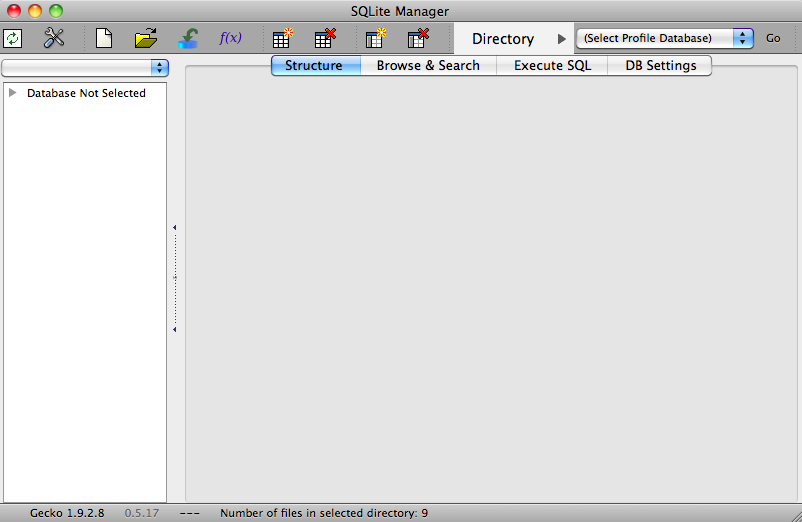
\includegraphics[width=15cm]{Figs/sqlitemanager.png}
  \caption{\label{sqlitemanagerrunning}SQLite Manger en Firefox}
\end{figure}

Aquí podemos empezar a manipular bases de datos relacionales usando el motor \Verb+sqlite3+.

Cree la base de datos PlnTFDB, haciendo click en el botón \textbf{New database}. Seleccione el directorio en donde desea guardarla, puede ser en el directorio \textbf{Documentos}.

Importe los archivos\footnote{Los archivos pueden ser descargados desde Sicua Plus} \Verb+tf.csv+, \Verb+Species.csv+, \Verb+Domains.csv+\footnote{Antes de importat abra cada uno de los archivos con un procesador de texto y defina que tipo de columnas aparecen, VARCHAR, NUMERIC, INTEGER, FLOAT} en las tablas TF, Species, y Domains respectivamente, usando la opción \textbf{import}, y asegurandose de seleccionar \Verb+Tab+ como el separador de campos e indicar que la primera fila consiste en los nombres de los campos. En el siguiente cuadro de diálogo indique el tipo de datos de cada columna.

Cree los siguientes indices\footnote{¿Para qué sirven los indices?}:

\begin{description}
\item[Tabla TF:]\textbf{Sp\_pepid} sin duplicados, como una clave primaria, \textbf{Sp\_ID} y \textbf{family\_id}
\item[Tabla Species:] \textbf{Sp\_ID} sin duplicados
\item[Tabla Domains:] \textbf{Sp\_pepid} con duplicados\footnote{¿Por qué es necesario aceptar duplicados?}, \textbf{domainid} con duplicados.
\end{description}

Relaciones entre las tablas: El campo Sp\_ID de la tabla TF está relacionado con el campo Sp\_ID de la tabla Species. El campo Sp\_pepid de la tabla Domains está relacionado con el campo Sp\_pepid de la tabla TF. ¿Que tipo de relación hay entre los campos: uno-a-uno, uno-a-varios, varios-a-varios? En este ejericio particular no los estamos usando, pero ¿qué son las claves externas (foreign keys)?

A manera de ejemplo vamos a realizar algunas conultas sencillas a la base de datos. Haga click en la pestaña \textbf{Execute SQL}, y en el cuadro \textbf{Enter SQL} escriba lo siguiente:

\begin{Verbatim}
 SELECT TF.Sp_pepid, TF.family_id, Species.Species_full_name 
   FROM TF, Species
     WHERE TF.Sp_ID=Species.Sp_ID 
\end{Verbatim}

Identifique las operaciones de \textbf{proyección}, \textbf{selección} y \textbf{conexión (JOIN)} en la anterior declaración SQL.

Vamos a hacer las siguientes consultas a la base de datos: \textcolor{red}{¿Cuáles son las familias de factores de transcripción presentes en las especies estudiadas?}

\begin{Verbatim}
 SELECT DISTINCT TF.family_id
   FROM TF
\end{Verbatim}

\textcolor{red}{¿Cuántas familias son?}

\begin{Verbatim}
 SELECT COUNT(DISTINCT TF.family_id)
   FROM TF
\end{Verbatim}

\textcolor{red}{¿Cuántas familias hay en cada especie?}
\begin{Verbatim}
 SELECT Species.Species_full_name, COUNT(DISTINCT TF.family_id)
   FROM TF, Species
     WHERE TF.Sp_ID=Species.Sp_ID
      GROUP BY Species.Sp_id
\end{Verbatim}

{\color{red}
Responda las siguientes preguntas:

\begin{enumerate}
\item ¿Cuántos genes por familia y por especie hay?
\item ¿Cuántos genes por especie hay?
\item ¿Que dominos están presentes en los genes de la familia MYB de la especie \textit{Arabidopsis thaliana}?
\item ¿Cuál es el número de dominios diferentes presentes en los genes de las diferentes especies?
\item ¿Cuál es la especie con mayor número de dominos diferentes?
\item ¿En que especie y gen se encuentra el dominio mas largo?
\item ¿Para qué sirve la expresión \Verb+limit+ en una declaración SQL en SQLite?
\end{enumerate}
}

\chapter{Búsquedas en base de datos biológicas - Segunda parte}

\section{PubMed}

Esta sección corresponde a una versión modificada del tutorial \url{http://www.nlm.nih.gov/bsd/disted/pubmedtutorial/}. Esta guía consiste en seguir el tutorial disponible en el enlace anterior y resolver las preguntas que aparecen mas abajo en rojo.

\textbf{PubMed} es la base de datos de literatura mantenida por el NCBI, actualmente tiene alrededor de 19 millones de registros.

\subsection{Entendiendo la información en los registros de PubMed}

Una referencia bibliográfica en PubMed está compuesta de campos que ofrecen información específica (Título, autor, lenguaje, etc) sobre el artículo publicado. La siguiente lista es una muestra de los campos que aparecen generalmente:

\begin{itemize}
\item Título del artículo
\item Nombres de los autores
\item Resumen publicado con el artículo
\item Vocabulario controlado de términos de búsqueda (Medical Subject Headings)
\item Información sobre la revista
\item Instituto o universidad a la que está afiliado el primer autor
\item Lenguaje en que el artículo fue publicado
\item Tipo de publicación (revisión, carta, nota pequeña, etc)
\item Identificador único de PubMed (PubMed Unique Identifier, PMID)
\end{itemize}

\textbf{Ejercicios}:

\begin{itemize}
\item \textcolor{red}{Haga una búsqueda en PubMed e identifique los campos que se mencionaron arriba.}
\item \textcolor{red}{Realize una búsqueda en PubMed con el término ``eye''. ¿Cuáles de los siguientes términos serán recuperados?}
 \begin{itemize}
  \item Eye, chin and forehead
  \item Eye, eyelids, cornea, iris, y todos los demás términos que estén subordinados al termino ``eye'' en MeSH.
   \item Eye (únicamente)
 \end{itemize}
 \item \textcolor{red}{¿Cuál fue la búsqueda exacta que realizó en el paso anterior? Pista: Ubique la caja de text ``\textbf{Search details}'' en la página de resultados.}
 \item \textcolor{red}{Haga una búsqueda en la base de datos MeSH usando como palabras clave sus áreas de interés e identifique los términos MeSH asociados.}
\end{itemize}

\textbf{Preguntas}

\begin{itemize}
\item \textcolor{red}{¿En que consiste el ``status'' de una entrada en PubMed?}
\item \textcolor{red}{¿Cuál es la diferencia entre MEDLINE y PubMed?}
\item \textcolor{red}{¿Qué son y para que sirven los términos MeSH?}
\item \textcolor{red}{Enq ue consiste ``Automatic Term Mapping''?}
\end{itemize}

\subsection{Realizando búsquedas}

Empleando la opción de búsqueda avanzada, usando la opción ``\textbf{Search builder}'', recupere todos los artículos científicos publicados por las profesoras Silvia Restrepo y Adriana Bernal desde el 2008 hasta el 2009, responda:

 \begin{itemize}
\item  \textcolor{red}{¿Cuántos artículos encontró?}
\item  \textcolor{red}{¿En que revistas fueron publicados?}
\item \textcolor{red}{¿A qué tipo de publicación corresponden?}
\item \textcolor{red}{¿Qué términos MeSH hay en común?}
\item \textcolor{red}{¿Qué términos MeSH reflejan el tema principal de los artículos?}
\item \textcolor{red}{Nombre tres referencias relacionadas al artículo mas reciente de la lista de resultados. ¿Cómo las identificó?}
\item \textcolor{red}{Envíe los resultados de su búsqueda a su correo electrónico, usando la opción ``\textbf{Send to}''}
\end{itemize}

\section{Descarga por lotes usando Entrez}

En aquellos casos en que se tiene un colección de identificadores de alguna base de datos consultada por Entrez, el sistema cuenta con una aplicación de descarga por lotes: ``Batch Entrez'' (\url{http://www.ncbi.nlm.nih.gov/sites/batchentrez})

Use el archivo \Verb+ID_list.txt+\footnote{Disponible en Sicua Plus} para hacer una consulta Batch Entrez y responda:

{\color{red}
\begin{itemize}
\item ¿Cuántos identificadores pueden ser recuperados por Entrez?
\item ¿En que base de datos se encuentran esos registros?
\item ¿Existe algún aviso importante para cualquiera de los registros? En caso afirmativo, explique en que consiste y por que puede pasar.
\item Enumere los pasos a seguir para cambiar la visualización de los registros y obtener las secuencias en formato Fasta y descargarlas en un archivo de texto.
\end{itemize}
}

\section{Recuperar todas las secuencias de un organismo o taxon}

En algunas ocasiones es necesario recuperar del NCBI todas las secuencias de ácidos nucleicos o de proteínas para una especie particular o para un grupo de organismos que pertenecen al mismo grupo taxonómico. Podemos empleada el ``Taxonomy Browser'' del NCBI para simplificar este proceso.

Haga una búsqueda en la base de datos de taxonomía usando \textit{Ornithorhynchus anatinus} como especie de interés. Los nombres vulgares comunes pueden ser usados, pero siempre es preferible emplear el nombre científico.  Al llegar al registro para la especie identifique su clasificación taxonómica. El número de registros en cada una de las bases de datos para la especie o grupo seleccionado, aparece como un enlace en la parte derecha de la página de resultados. Siguiendo esos enlaces puede descarga el conjunto completo de secuencias de la base de datos correspondiente.

Responda:

{\color{red}
\begin{itemize}
\item ¿Cuantas proteínas se encuentran?
\item ¿Cuántas secuencias de ácidos nucleicos?
\item ¿Qué otro tipo de información podría extraer?
\end{itemize}
}

\section{Recuperar la información publicada sobre un gen}

Haga una búsqueda en alguna de las base de datos usando como palabra clave el nombre del gen de interés y el organismo, Por ejemplo, usando la base de datos ``Gene'':

\begin{verbatim}
tpo[sym] AND human[orgn]
\end{verbatim}

En la página de resultados, siga el enlace al gen deseado. Si no existe un registro para el gen en las bases de datos seleccionadas, haga una nueva búsqueda en todas las bases de datos ``All databases''.

Cuando encuentre el registro para el gen, identifique en la página de resultados el enlace  ``Link''. Haciendo clic en este enlace desplegará una lista con mas enlaces, seleccione PubMed. Allí encontrará los registros de la base de datos de literatura que hacen referencia a su gen de interés.

Haga una búsqueda en la base de datos de ``Gene'' usando el nombre de gen ``ANAC092'' en la especie \textit{Arabidopsis thaliana}.


\begin{itemize}
\item \textcolor{red}{¿Que artículos en pubmed hacen referencia a ese gen?}
\item \textcolor{red}{Describa el gen usando la información encontrada en la base de datos ``Gene''}
\end{itemize}

\section{Bases de datos en el European Bioinformatics Institute (EBI)}

\subsection{SRS}

El ``Sequence Retrieval System'' (SRS) lo vimos en la Sección\ref{srs}. Siga el enlace \url{http://srs.ebi.ac.uk/srs/doc/index.html} y familiarícese con las opciones de búsqueda de este sistema.

\subsection{EB-eye}

Este es otro sistema de búsqueda en el EBI.

Haga una búsqueda en todas las bases de datos usando las palabras clave ``glutathione s-transferase'' en la página del EBI (\url{http://www.ebi.ac.uk/}). 

\textbf{Responda:}

{\color{red}
\begin{itemize}
\item Describa la página de resultados, ¿Cuántas bases de datos fueron consultadas? ¿En que categorías están agrupadas esas bases de datos?
\item ¿Cuántas y cuáles reacciones enzimáticas son mediadas por la enzima glutathione s-transferasa?
\item ¿Qué ontologías tienen registros asociados para la enzima? Descríbalas.
\item ¿Qué es una ontología? De ejemplos de algunas ontologías en biología
\end{itemize}
}

\section{Expasy}

El Expasy (\url{http://expasy.org/}) en el ``\textbf{Ex}pert \textbf{P}rotein \textbf{A}nalysis \textbf{Sy}stem'' mantenido por el Instituto Suizo de Bioinformática. Como su nombre lo indica está enfocado en el análisis de proteínas.

En esta sección vamos a usar algunas de las aplicaciones que se encuentran en el enlace \url{http://expasy.org/tools/}, principalmente aquellas con el logo del Expasy.

Use la secuencia de la proteína ANAC092 de \textit{Arabidopsis thaliana} para desarrollar los ejercicios de esta sección.

\textbf{Responda:}

{\color{red}
\begin{itemize}
\item ¿Cuál es el peso molecular y punto isoeléctrico de la proteína? ¿Qué herramienta usó para calcular esos parámetros?
\item ¿Cuántos y cuáles fragmentos se generan luego de una digestión con tripsina? ¿Qué herramienta uso para hacer la predicción? Calcule el punto isoelétrico y el peso molecular de cada fragmento.
\item Identifique la composición de amino ácidos de ANAC092. ¿Qué aplicaciones empleó?
\end{itemize}
}

\section{Mas ejercicios}

Encuentran mas guías siguiendo los enlaces \url{http://www.ncbi.nlm.nih.gov/guide/all/howto/} y \url{http://www.ebi.ac.uk/inc/help/search_help.html}.

\chapter{Ontologías en bioinformática: Gene Ontology}

Para desarrollar este capítulo tiene que leer la documentación sobre ``Gene Ontology'' siguiendo el enlace: \url{http://www.geneontology.org/GO.doc.shtml} y posiblemente seguir otros enlaces que allí se encuentren.

Parte de esta guía es una versión modificada del tutorial encontrado en el enlace: \url{http://www.geneontology.org/teaching_resources/tutorials/2007-10_GO-resources_jblake.doc}, pueden seguir independiente ese tutorial para desarrollar mas habilidades usando GO.

{\color{red}
\begin{itemize}
\item ¿Cuál es el objetivo del proyecto ``Gene Ontology'' (GO)?
\item Describa las tres ontologías que hacen parte de GO.
\item ¿En que consiste anotar un producto génico con términos GO?
\item Describa en que consisten las versiones ``Slim'' de GO.
\item ¿Cuál es la diferencia entre las ontologías y las anotaciones? Puede revisar los enlaces en la sección de descargas (``Downloads'').
\end{itemize}
}

Siga el enlace: \url{http://www.obofoundry.org/} de ``The Open Biological and Biomedical Ontologies''. {\color{red}Seleccione tres ontologías (diferentes a GO) que puedan ser útiles en su investigación y descríbalas brevemente.}

\section{Consultas en GO}

Vamos a usar ``AmiGO'' para hacer consultas a GO. AmiGO es un navegador basado en HTML que facilita la formulación de consultas tanto de las ontologías como de las asociaciones a los genes.

Haga una búsqueda de término usando ``carbohydrate metabolism''.

El resultado de la consulta muestra todos los términos que incluyen la cadena de caracteres ``carbohydrate metabolism''.  Haga clic en el primer término ``carbohydrate biosynthetic process''.

Lo primero que ve en cada línea es uno de los símbolos: $+$, $-$, o $\bullet$, como se muestra en la Figura~\ref{QueryGO5}. El símbolo $+$ puede ser usado para expandir un node, mostrando todos los hijos del término seleccionado. El símbolo $-$ puede ser usado para cerrar el nodo seleccionado. Finalmente $\bullet$ significa que el término no tiene hijos. Luego de esos símbolos va a encontrar las letras \textbf{P}, \textbf{I} o \textbf{R}, que identifican el tipo de relación: ``parte de'' (``part of''), ``es un'' (``is a''), o ``regula'' (``regulates''), repectivamente. Enseguida encuentra el identificador del término y el término. Al término le sigue un número en paréntesis que le indica el numero de productos génicos que ha sido anotados con ese término o a términos mas específicos (hijos).

\begin{figure}[ht]
\centering
   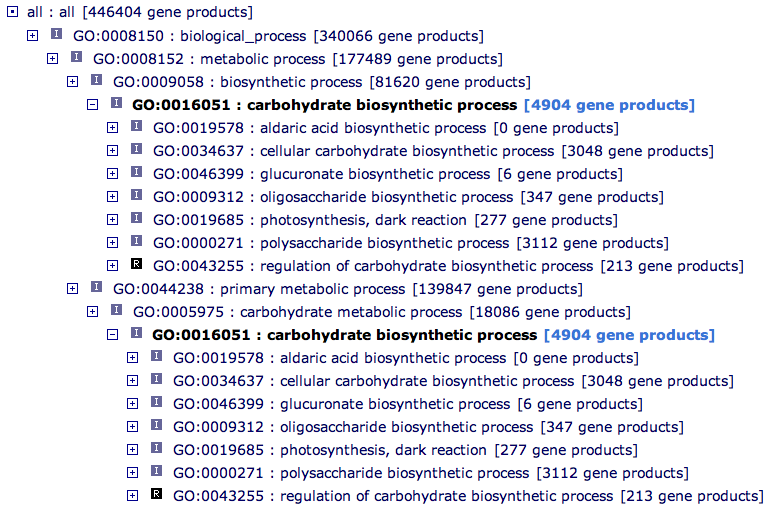
\includegraphics[width=15cm]{Figs/QueryGO5.png}
  \caption{\label{QueryGO5}Consultas en ``Gene Ontology''}
\end{figure}

Busque la opción ``Graphical View'' para visualizar esta sección de GO como un grafo acíclico dirigido, como el que se muestra en el Figura~\ref{GO_DAG}.

\begin{figure}[ht]
\centering
   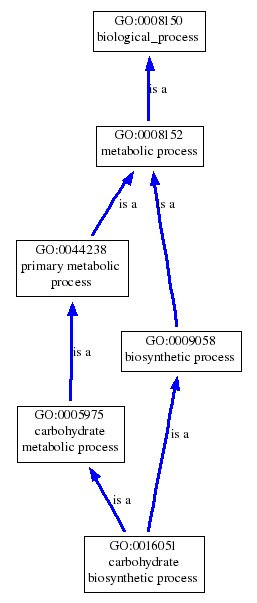
\includegraphics[height=8cm]{Figs/GO_DAG.png}
  \caption{\label{GO_DAG}Visualización del grafo acíclico dirigido de una sección de GO}
\end{figure}


Vamos a realizar otra consulta en GO usando como palabra clave el nombre de un gen (``ANAC092''), como se muestra en la Figura~\ref{QueryGO}.

\begin{figure}[ht]
\centering
   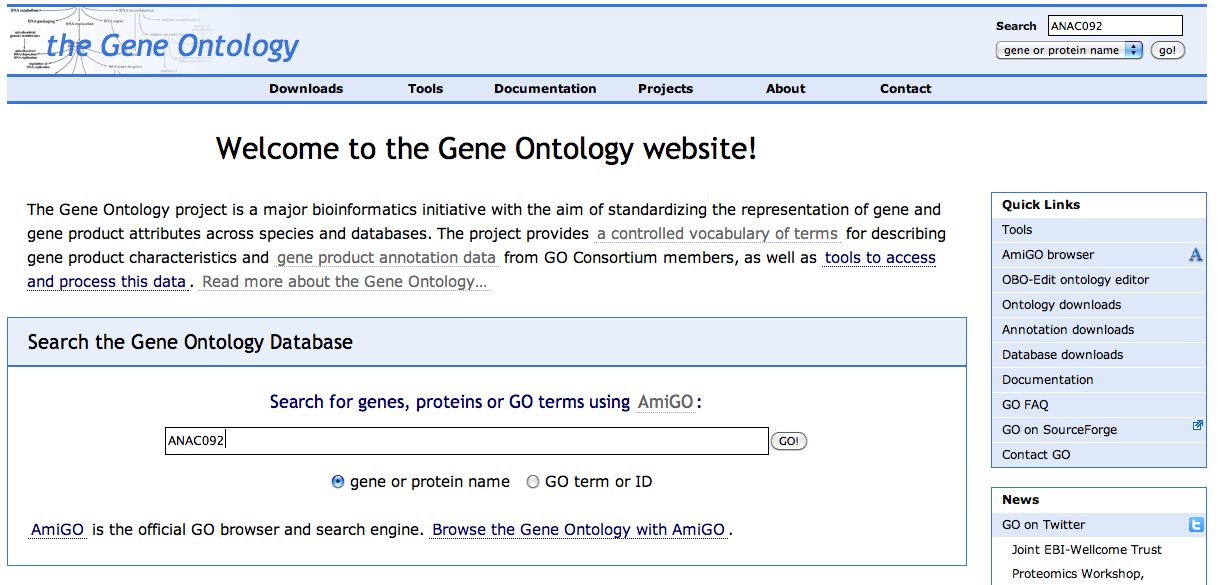
\includegraphics[width=15cm]{Figs/QueryGO1.png}
  \caption{\label{QueryGO}Consultas en ``Gene Ontology''}
\end{figure}

Ya que la búsqueda que realizamos fue muy específica, los resultados nos llevan directamente a la página de descripción de este gen en GO (Figura~\ref{QueryGO2}). El nombre del gen que usamos, ANAC092, no se encuentra en ninguna otra especie cubierta por GO. En esta página de resultados identifique la sección ``Term associations'' y siga el enlace, allí encontraremos el conjunto de términos GO que han sido asignados a este gen en particular, ver Figura~\ref{QueryGO3}.

\begin{figure}[ht]
\centering
   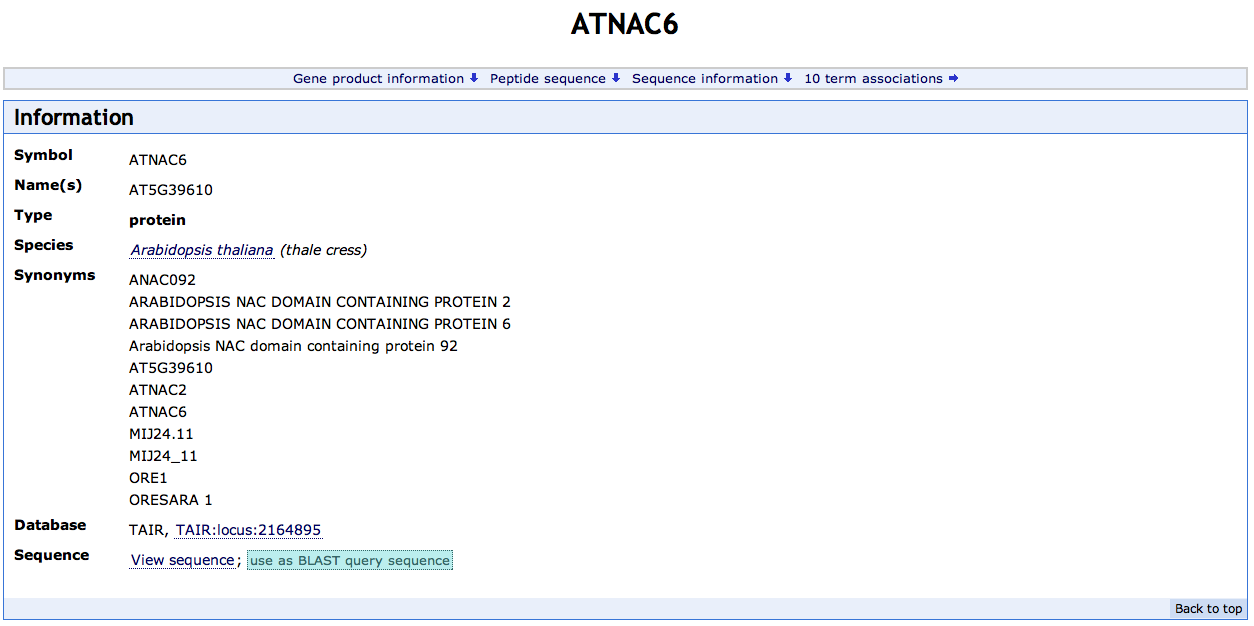
\includegraphics[width=15cm]{Figs/QueryGO2.png}
  \caption{\label{QueryGO2}Resultados de la consulta en ``Gene Ontology'', usando el nombre de gen ANAC092}
\end{figure}

\begin{figure}[ht]
\centering
   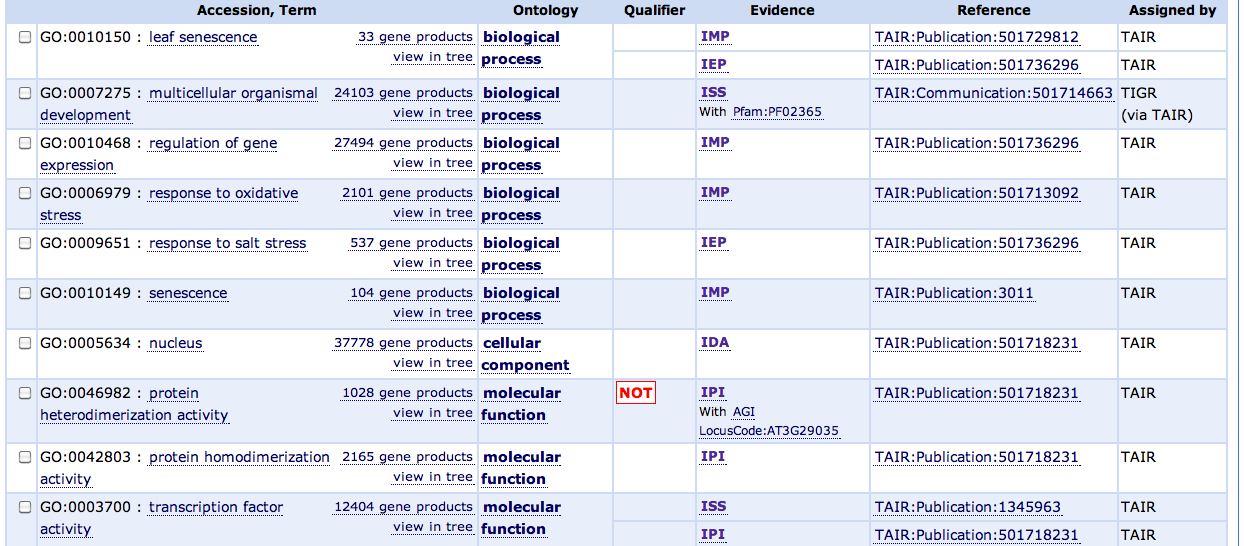
\includegraphics[width=15cm]{Figs/QueryGO3.png}
  \caption{\label{QueryGO3}Términos GO asociados al gen ANAC092}
\end{figure}

Haga clic sobre el término \textbf{GO:0007275 : multicellular organismal development}. Esto lo conducirá a la página de detalles del término, donde encuentra toda la información disponible sobre el término: nombre e identificador, sinónimos que pueda tener, definición, su posición en la estructura de GO, referencias a bases de datos externas, y los productos génicos asociados a ese término.

{\color{red}
\begin{itemize}
\item Describa cada uno de los códigos de evidencia asociados a las anotaciones del gene ANAC092 que aparecen en la Figura~\ref{QueryGO3}
\item Haga una lista de los términos GO asociados con este gen. ¿Qué está indicando el calificador ``NOT''?
\item Describa brevemente la función de este gen.
\item Muestre el grafo acíclico dirigido para la sección que incluye el término \textbf{GO:0010150 : leaf senescence}
\end{itemize}
}

\chapter{Introducción al análisis de redes usando Cytoscape}

En este capítulo vamos a aprender a trabajar con Cytoscape\footnote{\url{http://www.cytoscape.org/}}. Sigan el tutorial básico que se encuentra en el enlace: \url{http://cytoscape.wodaklab.org/wiki/Presentations/Basic}. Van a encontrar Cytoscape instalado en sus computadores, así que no tienen que usar la opción de ``Java Web Start''.

De la sección ``Defining visual styles'' del Tutorial 1: Getting Started, responda:

{\color{red}
\begin{itemize}
\item En la subred que incluye los vecinos más cercano a TP53 ¿Cuál es el tipo mas común de lado/arista? ¿Cuál el menos común?
\item ¿Cuántos nodos y aristas hay en la red ``DNA replication'' que cargó desde Reactome?
\end{itemize}
}

Despues de seguir el Tutorial 4: Expression Analysis, responda:

{\color{red}
\begin{itemize}
\item ¿Cuáles son los valores de expresión en las condiciones (genes pertubados): Gal1, Gal4, and Gal80 para el gene de levadura: YOL051W?
\item ¿Cuáles son los vecinos mas cercanos a ese gen (First Neighbors)?
\end{itemize}
}

\chapter{Análisis de enriquecimiento de anotaciones de genes}

Siga el tutorial que esta disponible en el enlace:\url{http://www.psb.ugent.be/cbd/papers/BiNGO/Tutorial.html}

El archivo\Verb+SaltArabidopsis.txt+ que está disponible en Sicua Plus, tienen una lista de genes de Arabidopsis que reponden diferencialmente al tratamiento con sal, y que fueron identificados a traves de ensayos usando microarreglos de ADN.

{\color{red}Use BinGO para identificar los términos GO que aparecen sobre y sub representados para los genes que aparecen en el archivo \Verb+gene_list.txt+. Muestre  el grafo de los términos e interprete los resultados.}

\chapter{Comparação de Sequência I - Matrizes de pontos}

As matrizes de pontos (``Dot Plot'') são ferramentas exploratórias para comparar strings de texto, ou seja, sequências. Entre outros, eles nos permitem encontrar facilmente regiões repetidas em uma sequência comparando-a com ela mesma. Também podemos ter uma boa ideia da estrutura de um gene comparando a sequência de sua região de codificação com a sequência do locus onde se encontra.

Nesta seção, usaremos a implementação de matrizes de pontos do Instituto Suíço de Bioinformática, conhecida como Dot Let\footnote{\url{http://myhits.isb-sib.ch/cgi-bin/dotlet}}, que vemos na Figura~\ref{DotLet1}.

\begin{figure}[ht]
\centering
   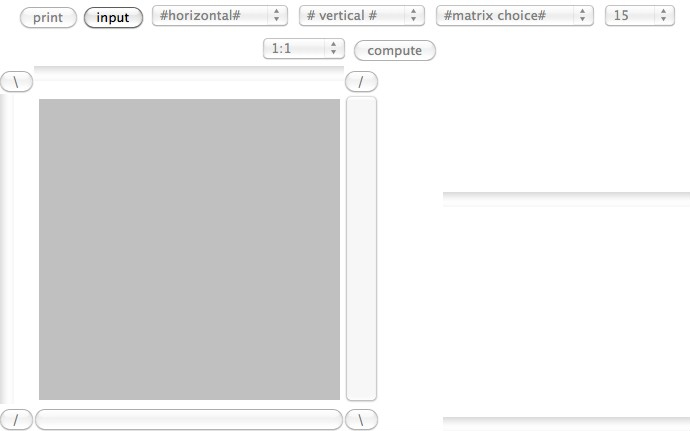
\includegraphics[width=10cm]{Figs/DotLet1.png}
  \caption{\label{DotLet1}Dot Let @ SIB}
\end{figure}

Faça uma comparação da sequência encontrada no arquivo \Verb+aqc-MIR399+ com ela mesma. A primeira coisa que você precisa fazer é clicar no botão ``Input'', que abrirá a janela mostrada na Figura~\ref{inputDotLet}, dar um nome à sequência e colá-la na caixa correspondente.

\begin{figure}[ht]
\centering
   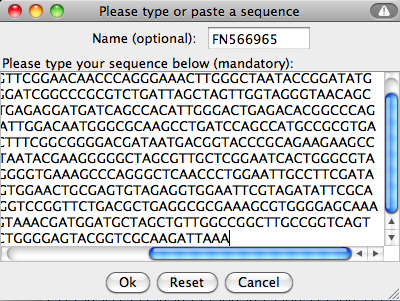
\includegraphics[width=7cm]{Figs/inputDotLet.png}
  \caption{\label{inputDotLet}Adicionar Sequências em Dot Let}
\end{figure}

De volta à janela Dot Let vemos que encontramos dois botões habilitados (Figura~\ref{DotLetbuttons}), eles agora aparecem com o nome da sequência que você acabou de adicionar. Uma delas representa a sequência que aparece na direção horizontal, a outra a sequência que aparece na direção vertical.

\begin{figure}[ht]
\centering
   
\includegraphics[width=10cm]{Figs/DotLetBotones.png}
  \caption{\label{DotLetbotones}botões de controle}
\end{figure}


À direita dos botões/listas que identificam as sequências, encontramos uma lista suspensa, atualmente desabilitada, que permite selecionar a matriz de substituição. Em seguida, encontramos uma lista suspensa com os tamanhos de janela que serão usados para a comparação das duas sequências. O próximo botão permite ampliar, ou seja, ``Zoom'', e finalmente encontramos o botão ``Calcular'', que preenche a matriz de pontos.

Uma vez que a matriz de pontos foi calculada, encontramos duas seções de resultados, semelhantes ao que aparece na Figura~\ref{DotLetResultado1}. A região da esquerda é a própria matriz, pixels escuros representam pontuações baixas, ou seja, ruins. À esquerda vemos um histograma da frequência de cada pontuação. Manipulando este histograma, com as barras de rolagem horizontais (para cima e para baixo) podemos modificar a exibição da matriz de pontos.

\begin{figure}[ht]
\centering
   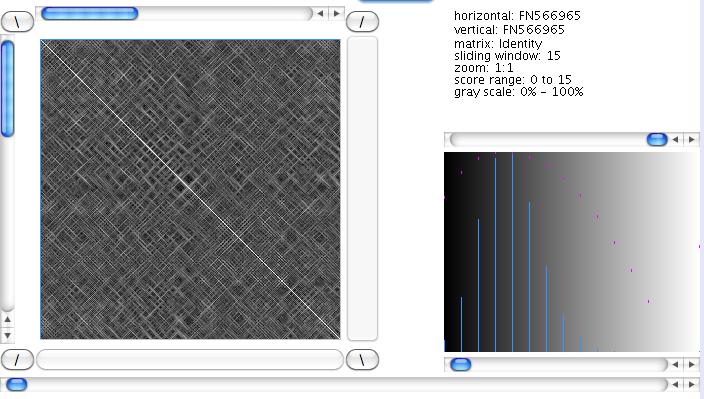
\includegraphics[width=15cm]{Figs/DotLetResultado1.png}
  \caption{\label{DotLetResultado1}Resultado}
\end{figure}

{\color{red}
\begin{itemize}
\item Explique como o tamanho da janela afeta a exibição na matriz de pontos.
\item Qual é o significado da linha rosa no histograma de pontuação?
\item Que interpretação você pode fazer das repetições invertidas que podem ser detectadas na matriz de pontos?
\item Compare a sequência de cDNA e sua contraparte genômica de ANAC092\footnote{Disponível em e-disciplinas}. Descreva os resultados.
\end{itemize}
}

\chapter{EMBOSS}

EMBOSS\footnote{\url{http://emboss.sourceforge.net/}},  ``The European Molecular Biology Open Software Suite'', é um pacote de código aberto gratuito composto por centenas de apps\footnote{\url{http://emboss.sourceforge.net/apps/release/6.6/emboss/apps/}} que foram desenvolvidos especificamente para atender às necessidades da comunidade de biologia molecular. O tutorial que você encontra abaixo faz parte dos tutoriais disponíveis em \url{http://emboss.sourceforge.net/docs/emboss_tutorial/emboss_tutorial.html}

Encontre uma descrição de cada um dos aplicativos presentes no EMBOSS seguindo o link: \url{http://emboss.sourceforge.net/apps/release/6.6/emboss/apps/}

Algumas das áreas abrangidas pelas aplicações EMBOSS são:

\begin{itemize}
\item Alinhamento de sequência
\item Pesquisar em bancos de dados usando padrões
\item Identificação de motivos proteicos
\item Análise de uso de códons
\end{itemize}

\section{Recuperando sequências de bancos de dados}

A recuperação de sequências de um banco de dados obviamente depende dos bancos de dados que temos disponíveis.

Vamos recuperar a sequência do gene ANAC092 do banco de dados de proteínas UniProt. Para fazer este exercício, você precisa ir ao site UniProt \footnote{\url{http://www.uniprot.org/}} e encontrar o identificador apropriado para baixar a sequência em formato .txt Figura~\ref{link_seq} usando wget (linha~\ref{getuniprot}).

\begin{Verbatim}[commandchars=!\{\},numbers=left,label=obtendo sequência do uniprot,frame=topline,fontsize=\scriptsize]
!textcolor{red}{[user@server]$} wget https://www.uniprot.org/uniprot/D7MJK1.txt !label{getuniprot}
--2022-04-06 14:23:06--  https://www.uniprot.org/uniprot/D7MJK1.txt
Resolving www.uniprot.org (www.uniprot.org)... 193.62.193.81
Connecting to www.uniprot.org (www.uniprot.org)|193.62.193.81|:443... connected.
HTTP request sent, awaiting response... 200 
Length: 4570 (4,5K) [text/plain]
Saving to: ‘D7MJK1.txt’
D7MJK1.txt          100%[===================>]   4,46K  --.-KB/s    in 0s      
2022-04-06 14:23:08 (275 MB/s) - ‘D7MJK1.txt’ saved [4570/4570]
\end{Verbatim} 

\begin{figure}[ht]
\centering
   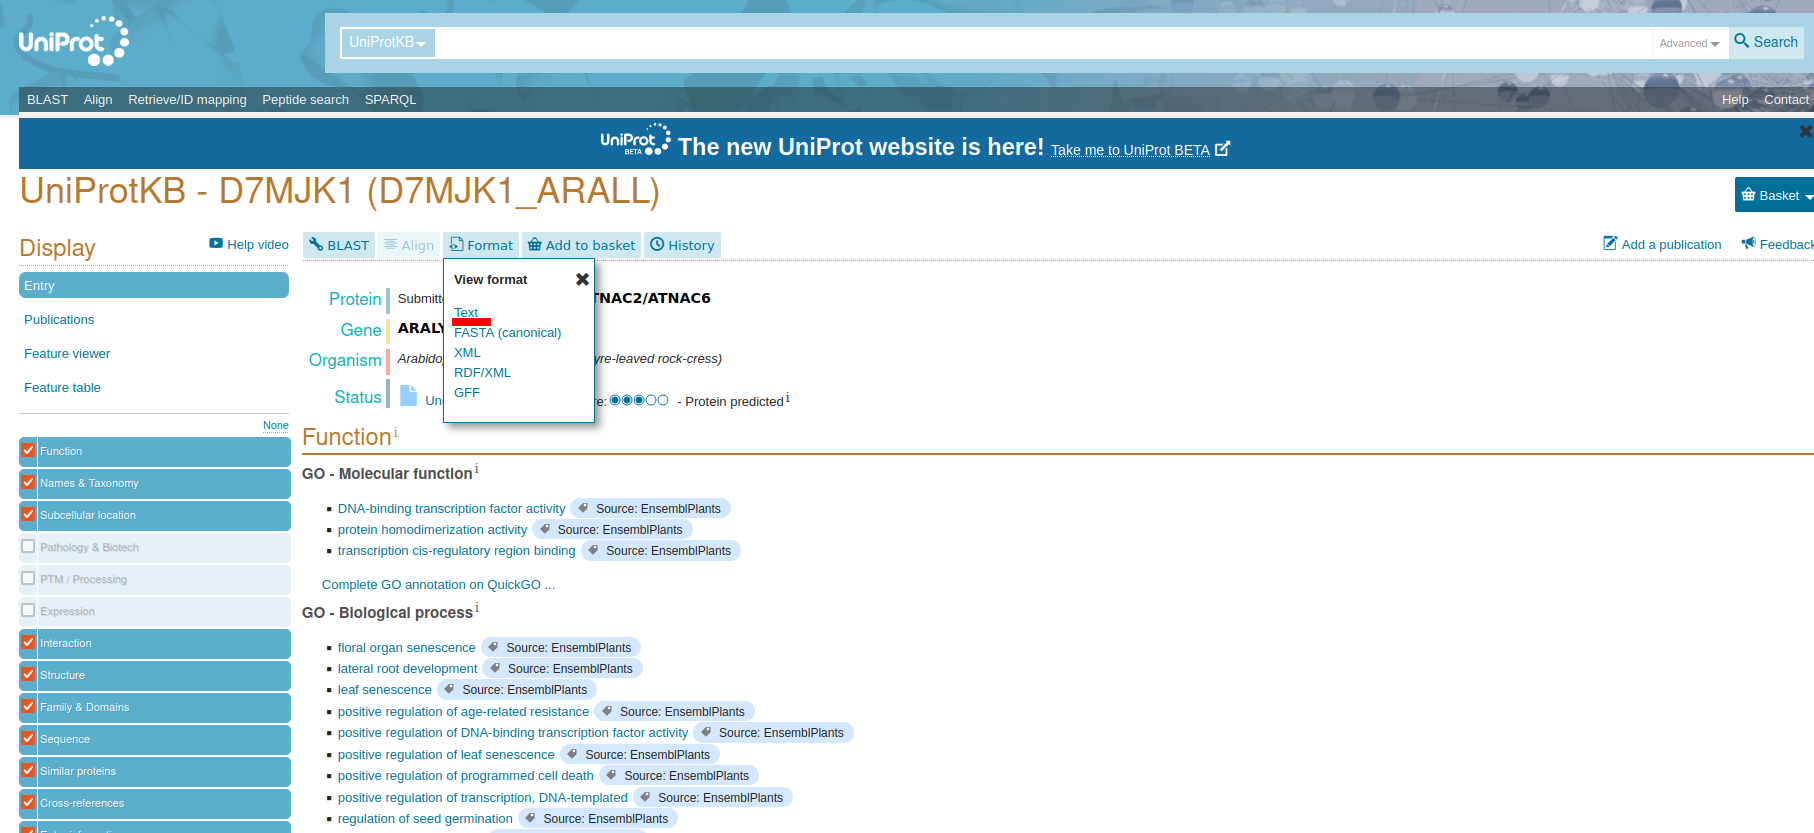
\includegraphics[width=12cm]{Figs/uniprot.png}
  \caption{\label{uniprot_site}Recuperando sequências de bancos de dados}
\end{figure}

\begin{figure}[ht]
\centering
   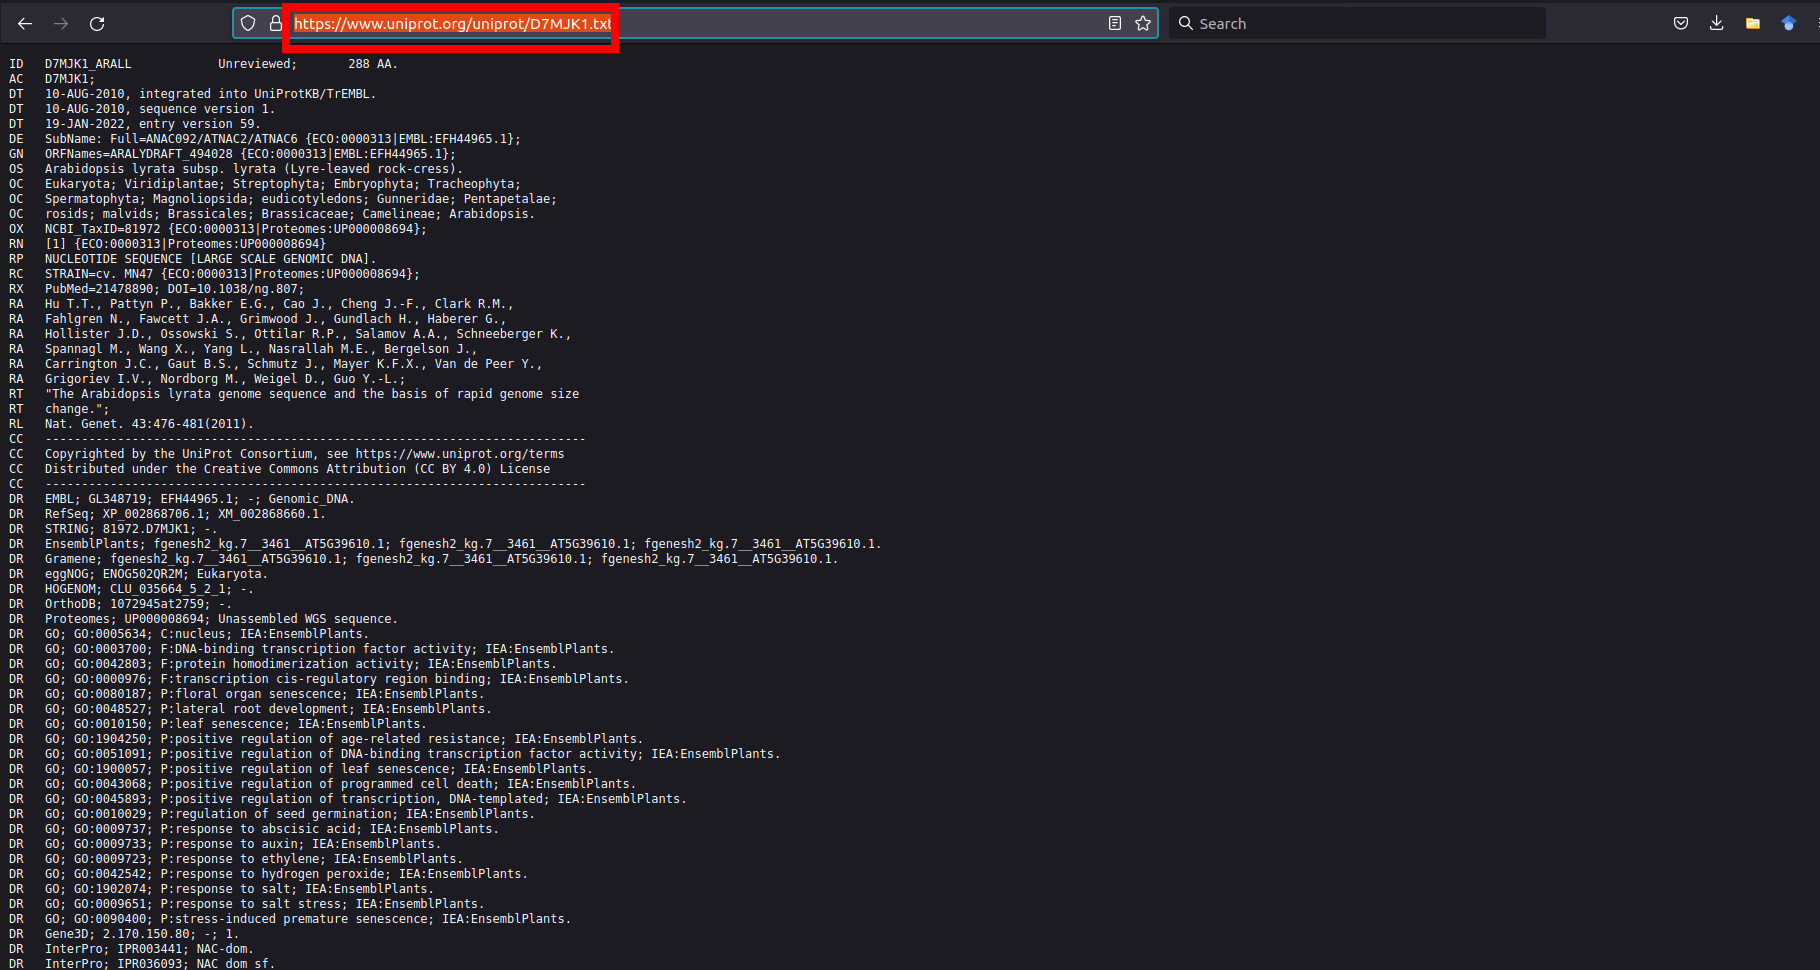
\includegraphics[width=12cm]{Figs/get_seq_link.png}
  \caption{\label{link_seq}Recuperando link de sequências em uniprot}
\end{figure}


O programa que nos interessa chama-se ``\Verb+seqret+''.

Agora, você pode usar o mesmo programa para converter a entrada recuperada do UniProt .txt para o formato fasta. \textcolor{red}{Como você faria isso?}

Já que você sabe como recuperar sequências do UniProt, vamos fazer alguns cálculos sobre essa sequência, procure o programa \Verb+compseq+, que permite calcular a composição da palavra de uma sequência. \textcolor{red}{Calcular frequências mais fracas para ANAC092 extraídas do UniProt}\footnote{Ao enviar seu guia esses resultados devem ser enviados em um arquivo de texto plano (.txt).}

\section{Seleção de quadros de leitura aberta}

Os programas \Verb+getorf+ e \Verb+plotorf+ buscam quadros de leitura abertos em sequências de nucleotídeos. Sendo um quadro de leitura aberto, uma sequência (subsequência) de um comprimento mínimo especificado flanqueado por dois códons de parada ou por um códon de partida e parada. Apesar da universalidade do código genético alguns grupos de organismos têm códons diferentes, por isso é importante especificar, seja o código genético que está sendo usado para traduzir a sequência, ou o início e parar códons permitidos.

{
\color{red}Use esses dois programas para encontrar o quadro de leitura aberto correto da sequência ''ANAC092\_cDNA.fa''\footnote{Arquivo \Verb+ANAC092\_cDNA.fa'+ disponível no e-disciplinas}. Você encontra alguma diferença nos resultados oferecidos pelos dois programas? 
}


\section{Embaralhar/misturar Sequências}

Ao fazer certos tipos de análise, por exemplo, procurar sites de vinculação de fatores de transcrição em sequências de promotores (``TFBS''), é importante ter um grupo de sequências que servem como um controle negativo. Para que o TFBS não apareça com frequência neste controle negativo. Uma opção amplamente utilizada é gerar sequências aleatórias que contenham a mesma composição monomérica das sequências originais. O programa ``shuffleseq'' faz exatamente isso, pega uma sequência ``real'' e mistura, como se embaralhando um baralho de cartas, os monômeros constituintes, resultando em uma sequência aleatória. Ao usar este tipo de estratégia, ~1000 sequências aleatórias são geradas para cada sequência original.

\textcolor{red}{Use ``shuffleseq'' para gerar duas sequências aleatórias do rRNA encontradas no arquivo \Verb+FN566965.fasta+ \footnote{Arquivo \Verb+FN566965.fasta+ disponível no e-disciplinas}}.

\section{Previsão de regiões hidrofóbicas} O programa \Verb+pepwindow+ prevê segmentos hidrofóbicos em uma proteína, seguindo a estratégia proposta por \citep{Kyte1982}. O uso de janelas de 19 a 21 resíduos regiões transmembranas pode ser claramente detectado, com valores de índice de hidroofobidade de 1,6 na região central.

\textcolor{red}{Pode detectar quaisquer regiões transmembranas no gene NTM1\footnote{Arquivo \Verb+NTM1.fasta+ disponível no e-disciplinas}?}

\section{Alinhamentos}

\textcolor{red}{Descreva a função do programa distmat}.

\chapter{Comparación de secuencias II - Alineamientos pareados}

Algunos apartes de este capítulo vienen del tutorial que se encuentra siguiendo el enlace: \url{http://emboss.sourceforge.net/docs/emboss_tutorial/emboss_tutorial.pdf}

Para desarrollar los ejercicios siga el enlace \url{http://mobyle.pasteur.fr/cgi-bin/portal.py}

\section{Matrices de sustitución}

En el archivo \Verb+EPAM250.txt+ encontrará la matriz de sustitución PAM250.

%Check: http://cnx.org/content/m11062/latest/

{
\color{red}
\begin{itemize}
\item ¿Quiénes, y cómo, crearon la familia de matrices de sustitución PAM?
\item ¿Dónde se encuentran los puntajes mas altos? Explique.
\item ¿Cuál es la sustitución con el mayor puntaje?
\item ¿Por qué las identidades  no tienen siempre el mismo puntaje?
\end{itemize}

}


\section{Alineamiento Global}

En el alineamiento global el objetivo es comparar las dos secuencias a lo largo de toda su longitud, por lo tanto, es apropiado cuando esperamos que la similitud entre las dos secuencias se extiende a lo largo de toda la secuencia.

En el paquete EMBOSS encontrará la aplicación \Verb+needle+ que implementa rigurosamente el algoritmo de  Needleman y Wunsch \citep{Needleman1970} para obtener el alineamiento global óptimo por programación dinámica. Esta implementación puede tomar bastante tiempo en obtener el alineamiento cuando las secuencias son largas.

\textcolor{red}{¿Qué otras aplicaciones en EMBOSS le permiten hacer alineamientos globales? ¿Qué las hace diferentes de \Verb+needle+?}

{\color{red}
\begin{itemize}
\item Haga un alineamiento global entre las secuencias de cDNA y genómica del gen ANAC092, que están disponibles en el directorio de la semana pasada en Sicua Plus.
\item ¿Qué matriz de sustitución y penalización para abrir y extender gaps usó? Explique.
\item ¿Cuál es el puntaje del alineamiento, su longitud y los porcentajes de identidad y similitud?
\item Explique la diferencia entre similitud e identidad.
\item ¿Qué significan los símbolos  \Verb+:+, \Verb+.+ y \Verb+|+?
\end{itemize}
}

En los archivos \Verb+ANAC092_pep.fasta+ y \Verb+PpNAC_e_gw1.5.134.1.fasta+ encuentra las secuencias de amino ácidos de dos genes de la familia NAC de factores de transcripción en \textit{Arabidopsis thaliana} y en el musgo \textit{Physcomitrella patens} respectivamente.

{\color{red}
\begin{itemize}
\item Haga un alineamiento global entre las secuencias de amino ácidos de las proteínas NAC de \textit{Arabidopsis thaliana} y en el musgo \textit{Physcomitrella patens}.
\item ¿Qué matriz de sustitución y penalización para abrir y extender gaps usó? Explique.
\item ¿Cuál es el puntaje del alineamiento, su longitud y los porcentajes de identidad y similitud?
\item ¿Puede mejorar el alineamiento escogiendo otros parámetros?
\end{itemize}
}

\section{Alineamientos locales}

Como se mencionó en la sección anterior el alineamiento global alinea a las secuencias a lo largo de toda su longitud. Usted tiene que decidir si esa estrategia es la mas adecuada en cada caso. \textcolor{red}{¿Qué cree que pasaría si compara dos proteínas multidominio que solo comparten un dominio entre ellas?}

El objetivo del alineamiento local es encontrar regiones de similitud local, y no es necesario incluir las secuencias completas. Este tipo de alineamiento es muy útil para hacer búsquedas en bases de datos, o cuando no se tiene una idea clara sobre la similitud de la secuencia de interés con secuencias de la base de datos.

En el paquete EMBOSS encontrará la aplicación \Verb+water+ que implementa rigurosamente el algoritmo de  smith y Waterman \citep{Smith1981} para obtener el alineamiento local óptimo por programación dinámica. Esta implementación puede tomar bastante tiempo en obtener el alineamiento cuando las secuencias son largas.

\textcolor{red}{¿Qué otras aplicaciones en EMBOSS le permiten hacer alineamientos locales? ¿Qué las hace diferentes de \Verb+water+?}

{\color{red}
\begin{itemize}
\item Haga un alineamiento local entre las secuencias de amino ácidos de las proteínas NAC de \textit{Arabidopsis thaliana} y en el musgo \textit{Physcomitrella patens}, que usó en la sección anterior.
\item ¿Qué matriz de sustitución y penalización para abrir y extender gaps usó? Explique.
\item ¿Cuál es el puntaje del alineamiento, su longitud y los porcentajes de identidad y similitud?
\item ¿Puede mejorar el alineamiento escogiendo otros parámetros?
\item ¿Qué diferencias hay entre el alineamiento global y el local de estas dos secuencias?
\end{itemize}
}

\section{Significancia de los alineamientos}

No importa que secuencias le de a los programas de alineamiento, ellos siempre crearan un alineamiento.

Tome la secuencias de amino ácidos ANAC092 y use el programa \Verb+shuffleseq+, y cree dos secuencias aleatorias con la misma composición monomérica de ANAC092. Haga un alineamiento global  y uno local con las dos secuencias.

{\color{red}
\begin{itemize}
\item ¿Qué matriz de sustitución y penalización para abrir y extender gaps usó? Explique.
\item ¿Cuál es el puntaje del alineamiento, su longitud y los porcentajes de identidad y similitud?
\item ¿Puede mejorar el alineamiento escogiendo otros parámetros?
\end{itemize}
}

Ahora haga un alineamiento local y uno global entre la secuencia de amino ácidos de ANAC092 y una de las versiones al azar.

{\color{red}
\begin{itemize}
\item ¿Qué matriz de sustitución y penalización para abrir y extender gaps usó? Explique.
\item ¿Cuál es el puntaje del alineamiento, su longitud y los porcentajes de identidad y similitud?
\item ¿Puede mejorar el alineamiento escogiendo otros parámetros?
\end{itemize}
}
%
%\chapter{\sc{Basic Local Alignment Search Tool}: BLAST}
%
%BLAST nos permite encontrar regiones de similitud local entre una secuencia de interés y secuencias de una base de datos.
%
%En este capítulo vamos a seguir una versión modificada del tutorial disponible en el enlace \url{http://www.ncbi.nlm.nih.gov/Education/BLASTinfo/tut1.html}.
%
%BLAST se encuentra en el enlace \url{http://blast.ncbi.nlm.nih.gov/Blast.cgi}
%
%Como ejemplo, considere la proteína MJ0577 (GI:2501594), de la archaea \textit{Methanococcus jannaschii}. La secuencia de amino ácidos se deriva del marco de lectura abierta MJ0577, y será usada como \textit{query} en la búsqueda de secuencias relacionadas en la base de datos de amino ácidos \Verb+nr+ (``non-redundant''). El programa \Verb+blastp+ es el apropiado para todo tipo de búsqueda en que la secuencia ``query'' es una proteína y se compara contra una base de datos de proteínas. La base de datos \Verb+nr+ es una buena opción para realizar una búsqueda inclusiva.
%
%Puede restringir su búsqueda a un organismo o grupo taxonómico usando la casilla de texto ``Organism''. En este caso no vamos a restringir la búsqueda a un organismo particular. Las relaciones que encontremos con proteínas de cualquier dominio de la vida nos darán pista sobre la función de la proteína de interés.
%
%En la sección de ``Algorithm parameters'' podemos seleccionar el valor E. Para este ejercicio lo vamos a cambiar del valor 10 que tiene por defecto a 1. A pesar de que los valores de E mayores que 0.1 no va reflejar verdaderas secuencias relacionadas, es útil para examinar hits con menor significancia de regiones cortas de similitud. En ausencia de similitudes mayores, esas regiones cortas nos pueden permitir hacer una asignación tentativa de las actividades bioquímicas de la proteína de interés. La significancia de esas regiones debe ser evaluada caso por caso.
%
%Cuando se está tratando de encontrar la función de una secuencia que no ha sido anotada, se deben mirar primero las secuencias homólogas en otros organismos que podrían ya estar anotadas. En segundo lugar se pueden mirar secuencias cortas que tienen alguna similitud con regiones de la secuencias de la base de datos que hayan sido caracterizadas bioquímicamente.
%
%La matriz de sustitución BLOSUM62 es una matriz de propósito general y es la opción por defecto en versiones actuales de BLAST. La matriz asigna un puntaje para cada posición en un alineamiento. Este puntaje esta basado en la frecuencia conque se observó dicha sustitución en bloques (alineamientos múltiples cortos) de proteínas relacionadas. BLOSUM62 está dentro de las mejores proteínas para detectar similitudes débiles entre proteínas.
%
%Las opciones de abrir y extender gaps dependen de la matriz de sustitución seleccionada. Por favor observe como cambiando de matriz estas opcioens cambian.
%
%A la derecha de cada opción en el formulario de búsqueda de BLAST encuentra un ícono de ayuda, al pincharlo obtendrá mas información sobre el parámetro o la opción en particular.
%

\chapter{BLAST: \sc{Basic Local Alignment Search Tool}}

Muchos de ustedes conocen la interfaz web de BLAST en el NCBI que se muestra en la Figura~\ref{blastx_input}.  En la primera parte de este tutorial vamos a hacer algunos ejercicios usando esta interfaz. 

\begin{figure}[h!]
\centering
   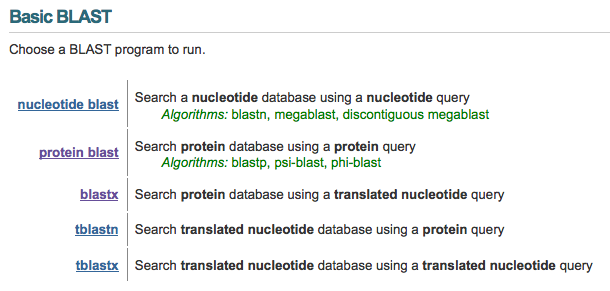
\includegraphics[width=10cm]{Figs/blasthomepage.png}
  \caption{\label{blasthomepage}Tipos de BLAST disponibles en el NCBI}
\end{figure}

En SicuaPlus encuentra el archivo \Verb+desconocido.nuc.fa+, que contiene la secuencia de nucleótidos de un transcrito que usted descubrió al analizar la expresión diferencial de genes de \textit{A. thaliana} en respuesta a luz ultravioleta (UV-A), tratamiento en el cual este transcrito era inducido. Copie la secuencia del transcrito y abra la página \url{http://blast.ncbi.nlm.nih.gov/} en el navegador Firefox. Vamos a realizar una búsqueda básica de BLAST, busque en la página una sección como la que aparece en la Figura~\ref{blasthomepage} y seleccione la opción \Verb+blastx+\textcolor{red}{{\textquestiondown}Por qué usar \Verb+blastx+?}

\begin{figure}[h!]
\centering
   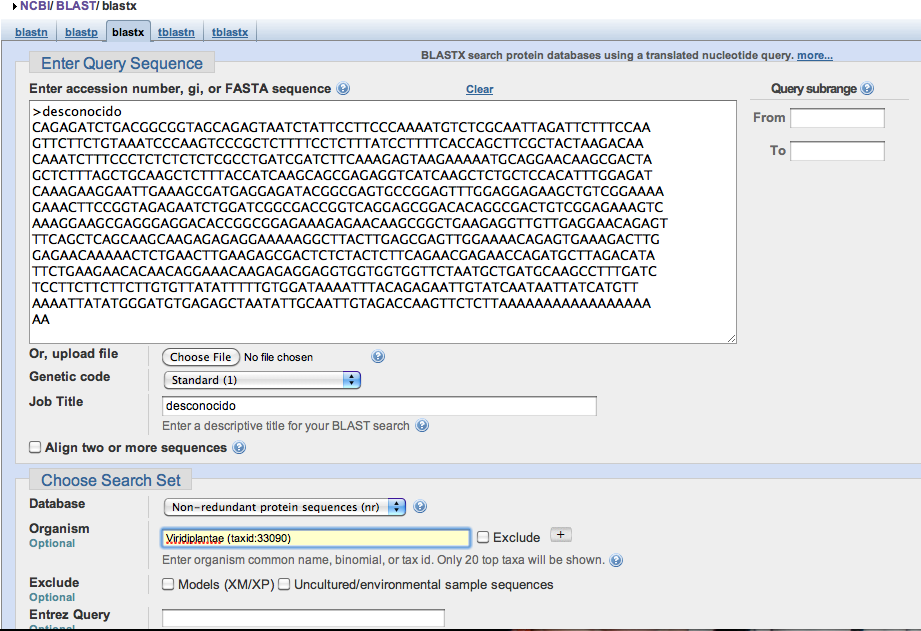
\includegraphics[width=10cm]{Figs/blastx_input.png}
  \caption{\label{blastx_input}Interfaz web de NCBI BLAST usando el programa blastx}
\end{figure}

En la página de \Verb+blastx+ pegue su secuencia desconocida en el campo ``\textbf{Enter query sequence}'', escriba \textit{Viridiplantae} en el campo ``\textbf{Organism}'', para restringir la búsqueda a las secuencias de plantas verdes (Figura~\ref{blastx_input}). Asegúrese de que la base de datos seleccionada sea la base de datos no redundante de secuencias de proteínas.

En las búsquedas que involucran la traducción en línea de una secuencia de ADN de puede seleccionar el código genético que se usará para hacer la traducción. Asegúrese que el código genético seleccionado en este caso es ``Standard''.

\begin{figure}[h!]
\centering
   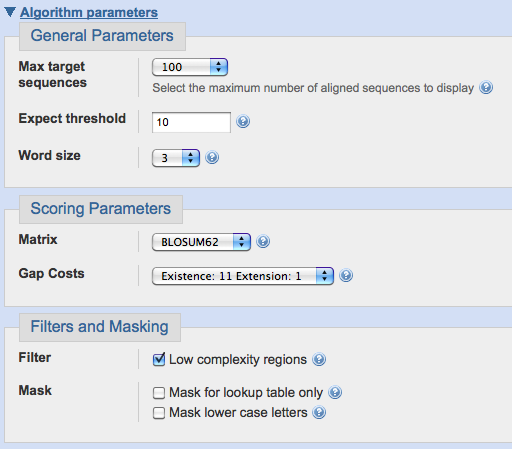
\includegraphics[width=10cm]{Figs/blastx_parameters.png}
  \caption{\label{blastx_parameters}Parámetros de búsqueda en BLAST}
\end{figure}

Un poco más abajo, haga click en el vínculo ``\textbf{Algorithm parameters}'', lo que le mostrará la serie de opciones que se ven en la Figura~\ref{blastx_parameters}. En la sección de ``\textbf{General parameters}'', encuentra el \textbf{Expected threshold} o \textbf{E value}. El E value es el número de alineamientos con un puntaje igual o mayor al obtenido que se espera que aparezcan por azar. En el momento de seleccionar los alineamientos importantes este es el parámetro mas importante; como regla general alineamientos con E value menor que $1\times10^{-5}$ representan secuencias homólogas. Sin embargo si está alineando secuencias muy cortas, e.g., 20 residuos, debe permitir alineamientos con un E value muy alto, alrededor de 100. En la sección ``\textbf{Scoring parameters}'', puede seleccionar la matriz de sustitución (escoja BLOSUM80) y la penalización por introducir gaps en el alineamiento.  Note que hay una diferencia entre el costo de introducir un gap y el de extenderlo \textcolor{red}{{\textquestiondown}A qué se debe esa diferencia?} Las opciones de abrir y extender gaps dependen de la matriz de sustitución seleccionada. Por favor observe como cambiando de matriz estas opciones cambian\footnote{En el enlace \url{http://www.ncbi.nlm.nih.gov/blast/html/sub_matrix.html} encontrará mayor información sobre la matriz de sustitución y la penalización de gaps.}.

Asegúrese que la opción \textbf{Filter} en la sección \textbf{Filters and Masking} esté seleccionada, con el fin de reducir el número de alineamientos con secuencias no relacionadas evolutivamente. \textcolor{red}{¿Qué programas usa BLAST para detectar regiones de baja complejidad?} \textcolor{red}{¿Qué funciones cumplen las opciones ``Mask for lookup table only'' y ``Mask lower case letters''?}

Ahora pinche el botón \textsc{BLAST} y espere sus resultados.

\begin{figure}[h!]
\centering
 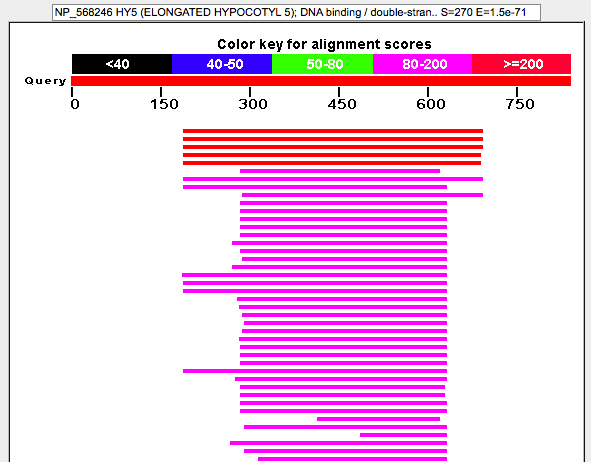
\includegraphics[width=9cm]{Figs/blastxres1.png}
  \caption[Resultados blast: gráfica]{\label{fig:blastxres1}Representación gráfica de los mejores alineamientos obtenidos en la búsqueda con \Verb+blastx+}
\end{figure}

\begin{figure}[h!]
\centering
 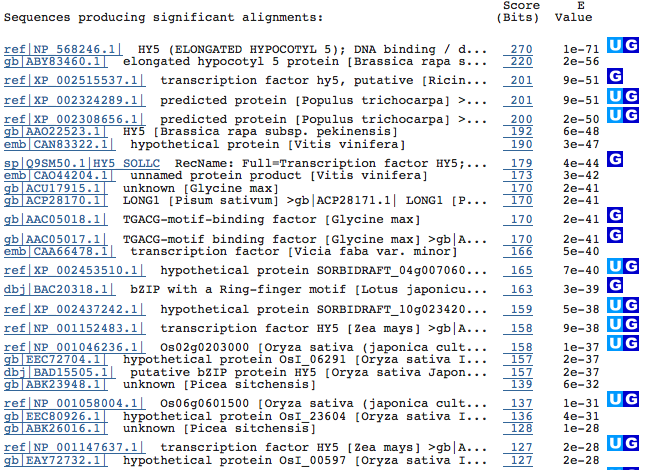
\includegraphics[width=9cm]{Figs/blastxres2.png}
 \caption[Resultados blast: hits]{\label{fig:blastxres2}Listado de ``Hits''}
\end{figure}

En la parte superior de la página de resultado encuentra una gráfica como la que se ve en la Figura~\ref{fig:blastxres1}. Consiste en una representación de los mejores alineamientos con un código de colores que representa la longitud del alineamiento.

Un poco mas abajo encuentra la tabla con  los mejores hits, donde se muestra el identificador (Accesion number) de la secuencia hit, parte de su descripción, el puntaje del alineamiento entre su secuencia desconocida y la secuencia de la base de datos, el porcentaje de la secuencia ``query'' que está representada en el alineamiento, la identidad y el E value. Puede re-ordenar los datos en esta tabla pinchando en los nombres de las columnas.

La última parte de la sección de resultados esta compuesta por los alineamientos propiamente dichos (Figura~\ref{fig:blastxres3}). Aquí va a encontrar nuevamente el puntaje y el E value del alineamiento. Adicionalmente, además del alineamiento, encuentra el número de posiciones en que las dos secuencias eran idénticas y similares (de acuerdo a la matriz de sustitución) y el número de gaps.

\textcolor{red}{¿Qué indican las regiones de los alineamientos que aparecen en gris y en minúscula?}

\begin{figure}[h!]
\centering
 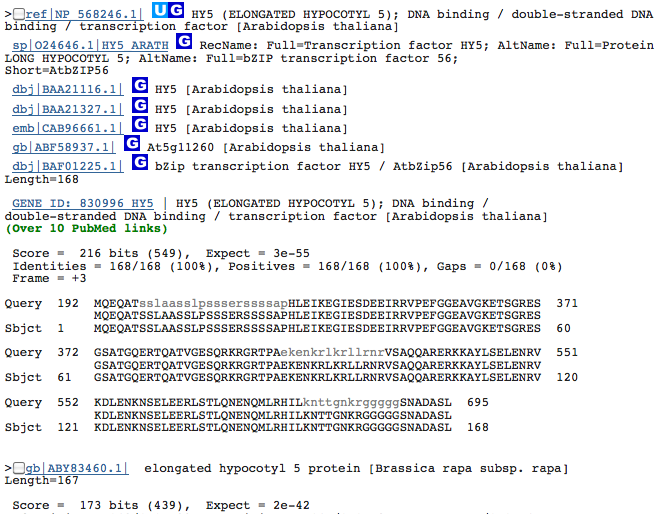
\includegraphics[width=9cm]{Figs/blastxres3.png}
 \caption[Resultados blast: alineamientos]{\label{fig:blastxres3}Alineamientos resultantes de la búsqueda con \Verb+blastx+}
\end{figure}

\textcolor{red}{{\textquestiondown}Qué puede decir sobre la función de su transcrito?}

La interfaz web de NCBI BLAST es muy amigable, pero tiene un par de problemas cuando trabajamos en genómica y proteómica, (i) no se pueden hace búsquedas contra bases de datos personalizadas o privadas y (ii) el número de secuencias que puede usar como \textbf{query} en cada búsqueda está restringido. La alternativa más poderosa para solucionar ambos problemas es instalar NCBI BLAST en un computador  local y configurar las bases de datos sobre las cuales se quiere realizar búsquedas (ver sección \ref{BlastCLI}).

\section{Encontrando la región genómica de un transcrito.}

Use la secuencia que se encuentra en el archivo \Verb+desconocido.nuc.fa+ para hacer una búsqueda BLAST, usando \Verb+blastn+ contra el genoma completo de \textit{A. thaliana}.  \textcolor{red}{¿Que opciones tiene que seleccionar para restringir su búsqueda a los cromosomas de \textit{Arabidopsis thaliana}?} Ya que BLAST realiza la búsqueda usando alineamientos locales, este resultado solo le dará una idea muy preliminar de la ubicación del transcrito en el genoma. Pero puede usar esta información para refinar la predicción del locus del transcrito usando \Verb+est2genome+ de EMBOSS. 

\textcolor{red}{¿Que opciones seleccionó para hacer la búsqueda en BLAST?¿Por qué?}

\textcolor{red}{Describa los resultados de la búsqueda.}

Los resultados de esta búsqueda nos permiten concluir que el locus del transcrito está en el cromosoma número 5 de \textit{A. thaliana}. \textcolor{red}{{\textquestiondown}Cuáles son las coordenadas aproximadas en el cromosoma? ¿Hay exones? Explique su respuesta.} Vamos a usar este resultado como entrada para \Verb+est2genome+. Primero extraiga de la secuencia del cromosoma 5, la región detectada por BLAST adicionándole $5000 pb$ corriente arriba y corriente abajo. \textcolor{red}{¿Cómo puede hacer esto?} Use \Verb+est2genome+ para refinar la predicción del locus. \textcolor{red}{{\textquestiondown}Qué ventajas ofrece usar \Verb+est2genome+ comparado con un simple BLAST?}

Para finalizar siga el enlace \url{http://www.ncbi.nlm.nih.gov/bookshelf/br.fcgi?book=comgen&part=psibl} y desarrolle el tutorial de PSI-BLAST.

\section{Blast$+$ en la línea de comandos}\label{BlastCLI}

Los ejecutables mas recientes, para diferentes platformas, de la suite Blast$+$ del NCBI los puede encontrar siguiendo el enlace \url{ftp://ftp.ncbi.nih.gov/blast/executables/blast+/LATEST}.

Para saber si la suite Blast$+$ está instalada en su computador ejecute el comando \Verb+blastp+, si la respuesta del sistema operativo es \Verb+comando no encontrado+ tendrá que descargar e instalar la suite Blast$+$. De lo contrario ya está listo para empezar a usar Blast$+$ desde la línea de comandos. 

Hay muchas opciones en los diferentes programas que componen la suite BLAST+, en este ejercicio solo tendremos tiempo de revisar unas pocas. Puede encontrar la documentación sobre estos en los siguientes enlaces:

\begin{itemize}
\item \url{http://blast.ncbi.nlm.nih.gov/Blast.cgi?CMD=Web&PAGE_TYPE=BlastDocs}
\item \url{http://www.ncbi.nlm.nih.gov/books/NBK1763/#CmdLineAppsManual.5_Cookbook}
\item \url{http://www.ncbi.nlm.nih.gov/books/NBK1763/#CmdLineAppsManual.4_User_manual}
\end{itemize}

Para desarrollar el ejercicio de hoy, descargue el archivo \Verb+TAIR10_pep_20101214.gz+ y descomprimalo como se muestra en la línea~\ref{downTAIRBLASTDB}. En este archivo encuentra todas las proteínas anotadas de \textit{Arabidopsis thaliana} correspondientes a la versión 10 de la anotación del genoma. Descargue las secuencias, en formato FastA, con números de acceso $BAK64065$ y $XP\_002889081$. Su objetivo es encontrar el mejor hit en la base de datos de proteínas de \textit{A. thaliana}, usando BLAST desde la línea de comandos.

\begin{Verbatim}[commandchars=!\{\},numbers=left,firstnumber=1,label=Ejecutando Blast+ en CLI,frame=topline,fontsize=\scriptsize]
!textcolor{red}{[user@server:~]$} mkdir ejercicio_blast
!textcolor{red}{[user@server:~]$} cd ejercicio_blast
!textcolor{red}{[user@server:~]$} wget http://biocomp-cms.uniandes.edu.co/exchange/TAIR10_pep_20101214.gz !label{downTAIRBLASTDB}
!textcolor{red}{[user@server:~]$} gunzip TAIR10_pep_20101214.gz
!textcolor{red}{[user@server:~]$} makeblastdb -in TAIR10_pep_20101214 -dbtype prot -parse_seqids -taxid 3702!label{makeblastdb}
!textcolor{red}{[user@server:~]$} blastp -query BAK64065.fasta -task blastp -db TAIR10_pep_20101214 \\ !label{blastpBAK64065}
-out BAK64065.blastp.out.txt -evalue 1e-5 -matrix BLOSUM62 -num_descriptions 1 -num_alignments 1
!textcolor{red}{[user@server:~]$} blastp -query BAK64065.fasta -task blastp -db TAIR10_pep_20101214 \\!label{blastpBAK64065TBL}
-out BAK64065.blastp.out.xml -evalue 1e-5 -matrix BLOSUM62 -num_descriptions 1 -num_alignments 1 \\
-outfmt 7
!textcolor{red}{[user@server:~]$}
!textcolor{red}{[user@server:~]$}
!textcolor{red}{[user@server:~]$}
!textcolor{red}{[user@server:~]$}
!textcolor{red}{[user@server:~]$}
\end{Verbatim} 

Antes de poder hacer búsquedas usando BLAST es necesario reformatear lel archivo que nos va a servir como base de datos. El comando \Verb+makeblastdb+ que  se distrubuye con la suite BLAST+ es el encargado de realizar esta tarea. En general para obtener información sobre como usar diferentes programas de la suite puede ejecutar \Verb+nombre_programa -help+. La línea~\ref{makeblastdb}, muestra el comando que debe ejecutar para crear la base de datos en formato blast. \textcolor{red}{¿Para que sirven cada uno de los argumentos que se pasan al programa \Verb+makeblastdb+?}

Teniendo la base de datos en el formato adecuado podemos hacer nuestra primera búsqueda. Use la secuencia proteínas BAK64065. Usaremos el programa \Verb+blastp+, para buscar el mejor hit de una proteína en una base de datos de proteínas (Línea~\ref{blastpBAK64065}). \textcolor{red}{¿Para que sirven cada uno de los argumentos que se pasan al programa \Verb+blastp+?}. Revise el archivo de salida, lo puede hacer con cualquiera de los siguientes comandos: \Verb+pico+, \Verb+less+. En la línea~\ref{blastpBAK64065TBL}, encuentra básicamente el mismo comando, solo que esta vez pedimos que el formato de salida sea tabular con la opción \Verb+-outfmt 7+. Hay muchos otros formatos de salida que se pueden pedir durante la búsqueda con el parámetro \Verb+-outfmt+. \textcolor{red}{Describa los formatos de salida posibles}.

\textcolor{red}{Haga la búsqueda con \Verb+blastp+ para la secuencia con número de acceso $XP\_002889081$, solo muestre los primeros 3 hits con e-value igual o menor que $10^{-10}$. Asegúrese de solicitar un formato de salida tabular que incluya la longitud de las secuencias ``Query''y ``Subject''}.

\chapter{Alineamientos múltiples}

En teoría los algoritmos de programación dinámica que se describieron anteriormente para el caso de alineamientos pareados se pueden extender para el caso de un número arbitrario de secuencias.  En la práctica, esto resulta muy costoso computacionalmente, por lo que se han desarrollado otros algoritmos que implementan atajos en la búsqueda de los alineamientos óptimos (heurísticas). El desarrollo de algoritmos para el alineamiento múltiple de secuencias es una de las áreas mas dinámicas de la bioinformática.  Actualmente existen decenas de programas que implementan diferentes algoritmos \citetext{vea \citealp{Notredame2007} y \citealp{Lemey2009} para una revisión reciente del tema}.

En esta sesión vamos a desarrollar la práctica que se presenta en el capítulo 3 de \citealp{Lemey2009}.

En este ejercicio vamos a alinear las secuencias de los genes TRIM5$\alpha$ de diferentes especies de primates. TRIM5$\alpha$ es un factor de restricción viral que proteje a la mayoría de monos del viejo mundo (Cercopithecidae) de la infección con HIV.Estos datos fueron analizados originalmente por \citealp{Sawyer2005}. Vamos a usar métodos de alineamiento progresivo ({\sc ClustalX}), basado en consistencias ({\sc T-coffee}) y de refinamiento iterativo ({\sc Muscle}) para crear alineamientos múltiples de proteínas y luego vamos a comparar los resultados usando el servidor web {\sc AltaVist}. Vamos a crear los alineamientos de las secuencias de las proteínas, vamos a comparar los diferentes métodos y vamos a generar el alineameinto correspondiente a nivel de nucleótidos, terminando con la inspección y refinamiento manual del alineamiento.

\section{Alineando las secuencias de amino ácidos de TRIM5$\alpha$ de primates}

\subsection{{\sc ClustalX}}

Decargue el archivo \Verb+primatesAA.fasta+ del SicuaPlus, este archivo tiene 22 secuencias en formato fasta. Inicie el programa {\sc ClustalX} que se encuentra instalado localmente en su computador \citep{Thompson1994}. En {\sc ClustalX} abra el archivo con las secuencias usando \Verb+File+ $\longrightarrow$ \Verb+Load sequences+. La interfaz gráfica le permite al usuario navegar sobre las secuencias. Seleccione \Verb+Alignment+ $\longrightarrow$ \Verb+Do complete alignment+. {\sc ClustalX} lleva a cabo el alineamiento progresivo y crea como salidas el árbol guía (con extensión \Verb+dnd+) y el alineamiento en formato Clustal (con extensión \Verb+aln+). Es posible escoger un formato diferente de salida para el alineamiento, siguiendo el menú \Verb+Alignment+ $\longrightarrow$ \Verb+Output Format Options+, seleccionando por ejemplo el formato {\sc Phylip} que puede ser leído por muchos paquetes para inferencia filogenética.

Recuerde que el árbol guía construido por {\sc ClustalX} no debe ser usado para sacar conclusiones sobre las relaciones evolutivas entre los grupos que se están estudiando.

{\sc ClustalX} también permite cambiar algunos de lso parámetros del alineamiento (\Verb+Alignment+ $\longrightarrow$ \Verb+Alignment Parameters+). Desafortunadamente no existen reglas generales para escoger el mejor conjunto de parámetros en un caso particular. La mejor opción consiste en ensayo y error. Si un alineamiento tiene, por ejemplo, muchos gaps largos, el usuario podría intentar incrementar la penalización para abrir gaps y re-hacer el alineamiento. {\sc ClustalX} indica el grado de conservación, revise la parte de abajo de la ventana del alineamiento,, ese nivel de ocnservación puede ser usado para evaluar el alineamiento. Seleccionando \Verb+Quality+ $\longrightarrow$ \Verb+Calculate Low Scoring Segment+\footnote{Siga el enlace \url{http://bips.u-strasbg.fr/fr/Documentation/ClustalX/} para entender como se calculan los segmentos de bajos puntaje.} y \Verb+Quality+ $\longrightarrow$ \Verb+Show Low Scoring Segment+, es posible visualizar aquellas regiones del alineamiento que no son confiables, que podrían removerse o refinarse manualmente. Salve el alineamiento usando \Verb+File+ $\longrightarrow$ \Verb+Save Sequences+ y selecciones {\sc Fasta} como formato de salida, asegurese de cambiar el nombre del archivo de salida para evitar sobre-escribir el archivo original.

\subsection{{\sc T-Coffee}}

Aunque el programa {\sc T-Coffee} se puede instalar localmente en sus computadores, para desarrollar este ejercicio vamos a usar un servidor web. Siga el enalce \url{http://www.tcoffee.org/}. Selecione el formulario de envío regular para {\sc T-Coffee}, allí cargue su archivo, usando \Verb+Upload File+ o pegue las secuencias en la caja de texto de envío. Asegurese que la opción \Verb+Computation mode+ está en \Verb+regular+.  Recuerde que los alineamientos con {\sc T-Coffee} son mas costosos desde el punto de vista computacional, ya que usa un método basado en consistencias, y por lo tanto puede tomar mas tiempo que un alineamiento con {\sc ClustalX} \citep{Notredame2000}. Presiona el boton \Verb+Submit+ para ejecutar el programa. Cuando el procedimiento de alineamiento halla terminado sera direccionado a una nueva página con enlaces a los archivos de salida. Salve el alineamiento en formato fasta en su computador. El archivo \Verb+score_pdf+ contiene una versión del alineamiento coloreada dependiendo de la calidad, este archivo también está disponible en formato {\sc html}.

\subsection{{\sc Muscle}}

Para obtener el alineamiento por el método de refinamiento iterativo vamos a usar el programa {\sc Muscle} \citep{Edgar2004}. Este progrma también puede ser instalado localmente en su computador, en esta ocasión vamos a usar el servidor web disponible en el EBI, siga el enlace \url{http://www.ebi.ac.uk/Tools/muscle/index.html}, alli puede cargar su archivo de secuenicas usando la opción \Verb+Upload a file+. Asegurese que la salida aparecerá en formato Fasta. Gurade el archivo de salida en formato fasta en su computador.

\subsection{Comparar los alineamientos usando la herramienta web {\sc AltAVist}}

Para evaluar los diferentes alineamientos vamos a usar la herramienta {\sc AltAVist}, siga el enlace \url{http://bibiserv.techfak.uni-bielefeld.de/altavist/}. {\sc AltAVist} compara dos alineamientos alternativos y usa códigos de color par aindicar concordancias y conflictos. Las regiones donde ambos alineamientos coinciden generalmente se consideran mas confiables que las regiones en donde difieren. Esta misma forma de razonamiento se aplica de forma similar al análsis de grupos en árboles filogenéticos que han sido reconstruidos usando varios algoritmos. Grupos presentes en árboles obtenidos con diferentes métodos sonmas confialbes que aquellos que no estan presentes de forma consistente.

\begin{figure}[h!]
\centering
 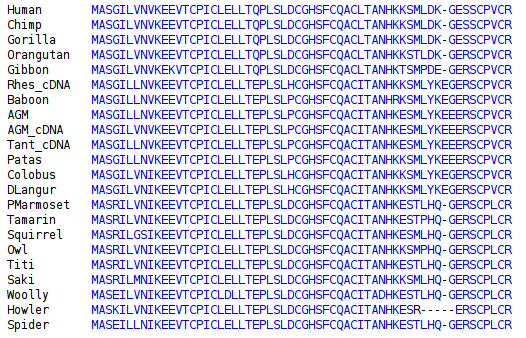
\includegraphics[width=9cm]{Figs/AltAVist1.png}
 \caption{\label{fig:AltAVist}Resultados de la comparación de alineamientos con {\sc AltAVist}}
\end{figure}

Para llevar a cabo el análisis siga el enlace anterior y seleccione \Verb+OPTION 2: Enter two+ \Verb+different pre-calculated alignments of a multiple sequence set+. Cargue sus dos alineamientos, empiece por el de {\sc ClustalX} y el de {\sc Muscle}, agregue los títulos correspondientes y presione el botón \Verb+Submit+. En la página de resultados aparecen los dos alineamientos con los residuos coloreados. La Figura~\ref{fig:AltAVist} muestra una de las regiones comparadas. Cuando todos los residuos en una columna son del mismo color , como es en la mayoría de los casos en la Figura~\ref{fig:AltAVist}, los residuos fueron alineados de la misma forma en los dos alineamientos. si un residuo tiene un color diferente, e.g., la arginina "R" para "Howler" en la posición $\pm 50$, está alinado de forma diferente en el segundo alineamiento.

diferentes colores se usan para distinguir diferentes grupos de residuos donde los alineamientos coinciden dentro de los grupos pero no entre grupos. Un ejemplo de esto se puede ver en la Figura~\ref{fig:AltAVist2}: los residuos \Verb+GSLT+ estan alineados por tanto por {\sc ClustalX} como por {\sc Muscle} de la misma forma en las \Verb+AGM+, \Verb+AGM_cDNA+ y \Verb+Tant_cDNA+, pero no con los mismos residuos en otros organismos. De forma similar ocurre para los residuos \Verb+TFPS+ y \Verb+SFPS+ en \Verb+Rhes_cDNA+ y \Verb+Babbon+, respectivamente; eso explica por que tienen color diferente.

\begin{figure}[h!]
\centering
 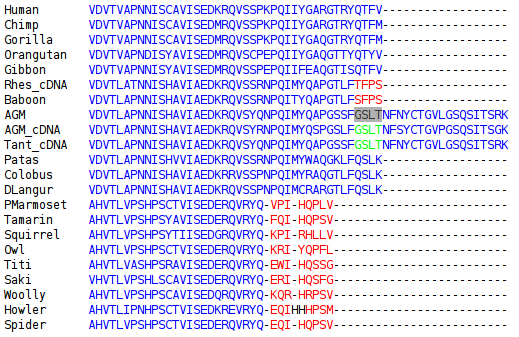
\includegraphics[width=9cm]{Figs/AltAVist2.png}
 \caption{\label{fig:AltAVist2}Resultados de la comparación de alineamientos con {\sc AltAVist}}
\end{figure}

Este tipo de análisis revela que algunos bloques de discrepancias en el alineamiento están concentrados cerca de las regiones con gaps. Por lo tanto, si las regiones con gaps se van a remover\footnote{Esto se suele hacer en los análisis filogenéticos}, es recomendable también borrar las regiones vecinas que tienen alineamientos ambiguos. \textcolor{red}{Haga todas las comparaciones entre los tres alineamientos que obtuvo anteriormente y describa brevemente las diferencias que observa. ¿Qué métodos de alineamientos presentan las mayores diferencias entre si? ¿Qué métodos las menores? Explique su respuesta}

\subsection{Del alineamiento de proteínas al de nucleótidos}

Los programas de alineamiento múltiple que se han mencionado generalmente rompen el marco de lctura cuando se alinean secuencias de ncleótidos. Esto invalidaría, por ejemplo, análisis posteriores  basados en codones, y necctarían de una buena dosis  de edición manual para restaurar los marcos de lectura. Para evitar esto, podemos usar el alineamiento basado en las secuencias de proteínas para generar el alineamiento correspondiente de nucleótidos. Este procedimiento también tiene la ventaja de que  los alineamientos de proteínas son menos ambiguos y mas rápidos de calcular.

Vamos a crear el alineamiento de las secuencias de ADN de TRIM5$\alpha$ usando la herramienta \Verb+RevTrans+ \citep{Wernersson2003}. Siga el enlace \url{http://www.cbs.dtu.dk/services/RevTrans/} y cargue el archivo con las secuencias de nucleótidos y uno de los alineamientos de proteínas. Revise que la opción \Verb+Match DNA and peptide sequences by+ sea igual a \Verb+Name+.

\textcolor{red}{¿Qué característica tienen los gaps en el alineamiento de las secuencias de ADN?\footnote{La característica se deriva de usar el alineamiento de proteínas como guía.}}

\subsection{Editando y visualizando alineamientos}

Vamos a usar la aplicación \Verb+JalView+ que está instalada en sus computadores para visualizar los alineamientos.

Siga el enlace \url{http://www.jalview.org/examples/editing.html}, si lo desea puede revisar la documentación completa en el enlace \url{http://www.jalview.org/help.html}. Identifique las regiones ambiguas del alineamiento (use la información que obtuvo al usar {\sc AltAVist} y eliminelas. \textcolor{red}{Muestre pantallazos de dos regiones que identifique como ambiguas. Explique por que las seleccionó y que región(es) descartó.}

\subsection{Estimando distancias entre las secuencias}
Cuando el objetivo es inferir las relaciones evolutivas entre las secuencias (o los organismos representados por las secuencias) a partir del alineamiento múltiple y usando un método de distancia\footnote{Hay cuatro grandes familias (métodos) de inferencia filogenética: métodos de distancia, de máxima verosimilitud, bayesianos y de máxima parsimonia.}, es necesario estimar una distancia evolutiva entre ellas. Hay muchos modelos para estimar las distancia evolutivas entre las secuencias, ya sean estas de ADN o de proteínas, por lo tanto es necesario escojer aquel modelo que mejor se ajuste a los datos \citep{Posada2001,Sullivan2005}. Se han desarrollado aplicaciones para automatizar y ayudar en la selección del mejor modelo siguiendo estrategías estadísticas; para secuencias de ADN existe {\sc ModelTest} \citep{Posada1998,Posada2006} y para secuencias de proteínas {\sc ProtTest} \citep{Abascal2005}.
  
Para ahorrrar tiempo, para este ejercicio vamos solo a estimar la distancia \textit{p} entre las secuencias que corresponde a la proporción de posiciones diferentes entre cada par de secuencia. En la realidad la distancia \textit{p} sub-estima el número real de sustituciones, ya que ignora el fenómeno de hits múltiples, i.e., que una posición dada puede haber sido sustituida mas de una vez. Los modelos que se mencionaron anteriormente implementan diferentes tipos de correcciones para tener esto en cuenta.
 
Vamos a usar la aplicación \Verb+protdist+ de {\sc Phylip}, un paquete para la inferencia de relaciones evolutivas, que está disponible en \url{http://mobyle.pasteur.fr/}. Siga el enlace anterior y busque la aplicación  \Verb+protdist+, selecciones la opción \Verb+File+ y cargue el archivo con su alineamiento múltiple de proteínas. Seleccione \Verb+Similarity table+ para el parámetro \Verb+Distance Model+, los demás parámetros los usamos con sus valores por defecto. Los valores en la matriz resultante indican la proporsición de posiciones identicas para cada par de secuencias. Para obtener la distancia, i.e., la proporción de posiciones diferentes entre cada par se secuencias, solo tenemos que restar el valor de la matriz a la unidad. Otra opción podría ser usar, por ejemplo, el programa MEGA4 \citep{Tamura2007}\footnote{\url{http://www.megasoftware.net/}}, que puede calcular directamente la proporción de posiciones diferentes.

\textcolor{red}{Identifique el par de primates mas cercanos y el par mas lejanos. ¿Cuáles son los valores en la matriz de distancia en los dos casos?}

\chapter{PSSMs, Logos de secuencias y HMMs}

\section{PSSM}

Esta sección es una versión modificada del tutorial que se encuentra siguiendo el enlace \url{http://rsat.ulb.ac.be/rsat/tutorials/tut_PSSM.html}.

Las ``Position-specific scoring matrices'' (PSSM) ofrecen una forma sensible de representar la variabilidad en un alineamiento. Las PSSMs se construyen tomando como base el alineamiento múltiple, e.g., de sitios de unión de factores de transcripción.

A continuación se muestra una matriz que fue obtenida de la base de promotores de \textit{Saccharomyces cerevisiae}\footnote{\url{http://rulai.cshl.edu/SCPD/}} y se construyó usando un alineamiento de 12 sitios de unión del factor de transcripción Pho4p de levadura.

\vskip5pt
\begin{center}
\begin{tabular}{l|r r r r r r r r r r }
A &  3 &  2 &  0 & 12 &  0 &  0 &  0 &  0 &  1 &  3\\
C &  5 &  2 & 12 &  0 & 12 &  0 &  1 &  0 &  2 &  1\\
G &  3 &  7 &  0 &  0 &  0 & 12 &  0 &  7 &  5 &  4\\
T &  1 &  1 &  0 &  0 &  0 &  0 & 11 &  5 &  4 &  4\\
\end{tabular}
\end{center}

Cada fila representa un residuo (A, C, g o T) y cada columna una posición en el conjunto de secuencias alineadas. Algunas posiciones están perfectamente conservadas en todas las secuencias, mientras que otras presentan algunas alternativas.

Cuando se usa este tipo de matrices para hacer búsquedas, las posiciones mas conservadas imponen restricciones mas fuertes que aquellas en que cualquier residuo se puede presentar.

{\color{red}
Siga el enlace \url{http://rulai.cshl.edu/cgi-bin/SCPD/getfactor?ABF1,BAF1} y responda:
\begin{itemize}
\item ¿Cuál es el tamaño del alfabeto?
\item ¿Cuál es el ancho de la matriz?
\item ¿Cuántos sitios de unión de Abf1p están almacenados en la base de datos de promotores de levadura (SCPD)?
\item ¿Qué programa(s) de EMBOSS podría usar para realizar búsquedas con PSSMs?
\end{itemize}
}

\section{Logos de secuencias}

Los logos de secuencias son una representación gráfica de los alineamientos múltiples basados en la teoría de la información\footnote{\url{http://www.ccrnp.ncifcrf.gov/~toms/glossary.html\#sequence_logo}}

La Figura~\ref{fig:lexALogo} corresponde al logo de secuencias de sitios de unión del factor de transcripción LexA de \textit{Escherichia coli}

\begin{figure}[h!]
\centering
 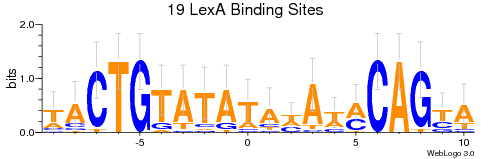
\includegraphics[width=9cm]{Figs/lexA.png}
 \caption{\label{fig:lexALogo}Logo de secuencias de los sitios de unión de LexA}
\end{figure}

La altura del residuo está correlacionada con su frecuencia en el alineamiento múltiple\footnote{Para mayor información consulte: \citealp{Schneider1990}}.

{\color{red}
Siguiendo el enlace \url{http://weblogo.threeplusone.com/}, cree el logo de secuencias de lo sitios de unión del factor de transcripción Abf1p que estudio en la sección anterior. Para poder realizar este ejercicio necesita recuperar todos los sitios de unión de Abf1p disponibles en SCPD.

¿Qué representa el eje y? i.e., ¿Cómo se calcula el contenido de información de cada posición?
}

\section{Modelos Ocultos de Markov: HMMs}

Vamos a seguir algunos de los ejemplos/ejercicios que se encuentran siguiendo el enlace \url{http://www.mrc-lmb.cam.ac.uk/rlw/text/bioinfo_tuto/structure.html}

Incluso si no encuentra proteínas homólogas al realizar una búsqueda con BLAST, todavía tiene otras opciones.

La principal razón por la cual no encuentra homólogos triviales es que las búsquedas con secuencias usando herramientas como BLAST tienen poca sensibilidad. BLAST normalmente no encuentra proteínas homólogas que tengan menos de 30\% de identidad. Sin embargo, algunas proteínas pueden tener la misma estructura tridimensional y tener solo 10\% de identidad.

Una estrategia muy útil para encontrar homólogos distantes está basada en el uso de Modelos Ocultos de Markov (HMMs). Un HMM no es mas que una forma de definir motivos o dominios.

Para crear un HMM todo lo que necesita es un alineamiento múltiple, el cual será usado para crear una representación probabilistica, que puede ser luego usada para buscar secuencias relacionadas.

Las bases de datos Pfam \citep{Finn2010} y {\sc Superfamily} \citep{Wilson2009} son colecciones de alineamientos múltiples para los cuales se han creado HMMs y son usadas para anotar secuencias de proteínas. La mayoría del trabajo de los curadores de esas bases de datos es crear los alineamientos múltiples.

\subsection{Buscando los dominios de una proteína}

Vamos a usar la siguiente proteína para hacer una búsqueda en Pfam:

\begin{Verbatim}[commandchars=!\{\},label=proteína desconocida,frame=topline,fontsize=\scriptsize]
>seq
MEYWHYVETTSSGQPLLREGEKDIFIDQSVGLYHGKSKILQRQRGRIFLTSQRIIYIDDAKPTQ
NSLGLELDDLAYVNYSSGFLTRSPRLILFFKDPSSKDELGKSAETASADVVSTWVCPICMVSNETQGEFTKD
TLPTPICINCGVPADYELTKSSINCSNAIDPNANPRNQFGVNSENICPACTFANHPQIGNCEICGHRLPNAS
KVRSKLNRLNFHDSRVHIELEKNSLARNKSSHSALSSSSSTGSSTEFVQLSFRKSDGVLFSQATERALENIL 
TEKNKHIFN
\end{Verbatim} 

Vaya al sitio web de Pfam\footnote{\url{http://pfam.sanger.ac.uk/}} y seleccione ``Sequence search'', pega la secuencia de la proteína de interés en la caja de texto para la búsqueda, luego haga clic en el botón ``go'' para iniciar la búsqueda. La Figura~\ref{PfamResults} muestra la página de resultados.

\begin{figure}[h!]
\centering
 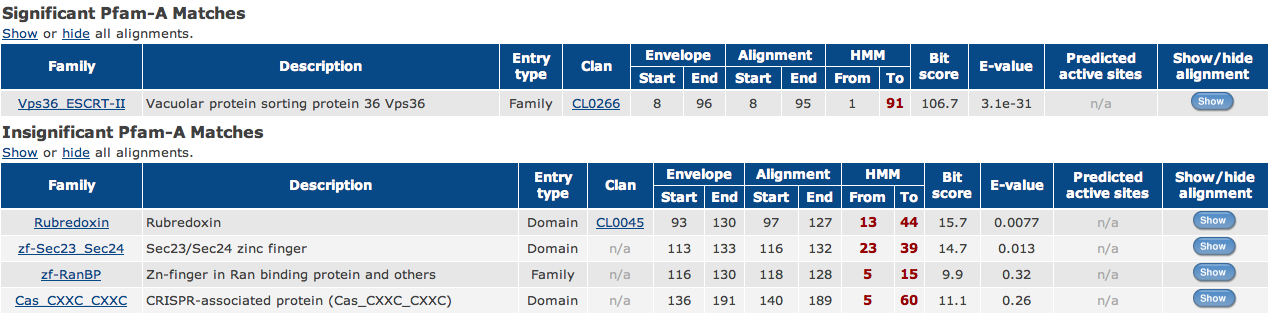
\includegraphics[width=14cm]{Figs/PfamResults.png}
 \caption{\label{PfamResults}Resultados de una búsqueda en Pfam}
\end{figure}

{\color{red}
\begin{itemize}
\item ¿Cuál es la diferencia entre ``Significant Pfam-A matches'' e ``Insignificant Pfam-A matches''?
\item ¿Qué es Pfam-A? 
\item ¿Qué es Pfam-B?
\end{itemize}
}

La primera sección de resultados ``Significant Pfam-A matches'', nos informa que hay un solo hit, al modelo ``Vps36\_ESCRT-II'', con un puntaje de $106.7$ y un e-value de $3.1e-31$. También encontramos las coordenadas del dominio, can relación a la proteína de consulta y con relación al modelo.

Una de las principales características, y valores agregados de Pfam, es que cada uno de los modelos en Pfam-A ha sido estudiado por un experto que ha definido una serie de puntajes límite para definir hits significativos. El puntaje umbral mas importante corresponde al ``gathering cutoff''. \textcolor{red}{¿Cuál el el Gathering cutoff del modelo ``Vps36\_ESCRT-II''?}

De clic en el nombre del modelo. Esto lo llevará a una página con información detallada sobre ese modelo particular. Entre otros, puede encontrar en que otras especies esta presente ese modelo (``Species''). Puede descargar el modelo (``Curation'') o el alineamiento múltiple (``Alignments''), entre otra información.

{\color{red}
Use la secuencia de la proteína ANAC092 y determine que dominios están presentes}

\subsection{Visualización de HMMs}

También puede visualizar los HMMs en forma de logos de secuencias. Puede usar la aplicación \Verb+LogoMat-M+ que encuentra en el enlace \url{http://www.sanger.ac.uk/cgi-bin/software/analysis/logomat-m.cgi}.

\textcolor{red}{Muestre el logo del dominio ``zf-C2H2''}

\chapter{Diseño de primers para PCR}

La parte teórica que aquí se presenta consiste en un resumen del texto que se encuentra siguiendo el enlace: \url{http://www.premierbiosoft.com/tech_notes/PCR_Primer_Design.html}.

La reacción en cadena de la polimerasa (PCR) inventada por Kary Mullis en la década de los 80s del siglo XX \citep{Mullis1987} es considerada uno de los inventos mas importantes en biología molecular. Mediante esta reacción pequeñas cantidades de material genético se pueden amplificar de tal forma que pueden ser identificadas y/o manipuladas.

La PCR involucra los siguientes pasos:

\begin{description}
\item[Denaturación] El objetivo de este paso es convertir las moléculas de ADN de doble cadena en cadenas sencillas.
\item[Anillamiento] Durante este paso los primers hibridan con las hebras molde de cadena sencilla.
\item[Extensión] La ADN polimerasa extiende los primers.
\end{description}

Esos pasos dependen y son muy sensibles a la temperatura. Las temperaturas usadas comúnmente son 95$^\circ$C, 60$^\circ$C y 72$^\circ$C, respectivamente.

Un buen diseño de primers es esencial para obtener reacciones exitosas. A continuación se describen las principales consideraciones a tener en cuenta durante el diseño.

\textbf{Longitud de los primers}: Normalmente se acepta que la longitud óptima para primers de PCR está entre 18 y 22 pb. Con esta longitud son lo suficientemente largos para asegurar especificidad y lo suficientemente pequeños para que se unan fácilmente al ADN molde a la temperatura de anillamiento.

\textbf{Temperatura de fusión del primer (T$_m$)}: Se define como la temperatura a la cual la mitad de las moléculas de ADN de doble cadena se van a disociar y volverse de cadena sencilla. Es una forma de indicar la estabilidad del duplex. Primers con temperaturas de fusión entre 52$^\circ$C y 58$^\circ$C normalmente producen los mejores resultados. Primers con temperaturas de fusión superiores a 65$^\circ$C tienen tendencia a formar anillamientos secundarios. El contenido de GC de la secuencia da una buena indicación de la temperatura de fusión del primer. Mayor precisión en su cálculo se alcanza empleado la teoría termodinámica de los vecinos mas cercanos, según la cual:

\begin{equation}
 T_m(^\circ C) = \lbrace\Delta H/\Delta S +Rln(C)\rbrace-273.15 \label{eq:tm}
\end{equation}

donde:

\begin{description}
\item[$\Delta H$ (kcal/mol)]: H es la entalpía. La entalpía es la cantidad de energía calórica que poseen las sustancias. $\Delta H$ es el cambio en entalpía. En la formula \ref{eq:tm}, la $\Delta H$ se obtiene de sumar las entalpías de los pares de di-nucleótidos que son vecinos mas cercanos.
\item[$\Delta S$ (kcal/mol)]: S es la cantidad de desornen deun sistema, recibe el nombre de entropía. $\Delta S$ es el cambio en la entropía. Se obtiene sumando las valores de entropía de pares de di-nucleótidos que son vecinos mas cercanos. Normalmente se adiciona una correción a los parámetros de vecinos mas cercanos. Esta corrección representa el contenido de sales.
\item[$\Delta S$ (corrección por sales)]: $ \Delta S (1M NaCl )+ 0.368  N  ln([Na+]) $, donde $N$ es el número de pares de nucleótidos en el primers, y $[Na+]$ son los equivalentes de sal en mM.
\end{description}

\textbf{Temperatura de anillamiento de los primers}: La T$_M$ es un estimador de la estabilidad del híbrido ADN-ADN y es importante para poder estimar la temperatura de anillamiento (T$_a$).  T$_a$ muy altas harán que se formes pocos híbridos primer - molde resultando en una reducción del producto de PCR.  T$_a$ muy bajas podrán causar anillamientos no específicos. La siguiente ecuación permite estimar la T$_a$ a partir de la T$_m$

\begin{equation}
T_a = 0.3  T_m(primer) + 0.7 T_m (product) – 14.9
\end{equation}

donde,

\begin{description}
\item[T$_m$(primer)]  Es la temperatura de fusión de los primers
\item[T$_m$(product)] Es la temperatura de fusión del producto
\end{description}

\textbf{Contenido de GC}: La proporción de G$+$C en el primer debe ser de 40\% a 60\%.

\textbf{Gancho de GC}: La presencia de las bases G o C en las ultimas 5 bases del extremo 3' del primer (GC clamp) ayuda a tener una unión mas especifica en ese extremos debido a la unión mas fuerte entre G  y C. Sin embargo, se deben evitar mas de 3 Gs o Cs consecutivas en las últimas 5 bases del extremo 3'.

\textbf{Estructuras secundarias de los primers}: La presencia de estructuras secundarias producidas por interacciones intra o intermoleculares puede llevar a una disminución en la producción del amplímero o no producción de este. Esas estructuras disminuyen la cantidad de primer disponible para la reacción.

\textbf{Evitar hidridación cruzada}: Los primers diseñados para una secuencias no deben amplificar otro gen en la mezcla. La opción mas común es tomar los primers candidatos y compararlos contra bases de datos de genes usando una herramienta como BLAST.

\section{Diseño de primers usando Quantprime}

{\sc Quantprime}\footnote{Hay un tutorial disponible en el sitio de {\sc Quantprime} que describe con mayor detalle cada paso y opción.} es una herramienta flexible para el diseño de primers a mediana y gran escala \citep{Arvidsson2008}, principalmente para PCR en tiempo real usando SYBR GREEN. {\sc Quantprime} usa \Verb+primer3+ \citep{Rozen2000}  como motor para la creación de primers y agrega diversas capaz de verificación contra distintas bases de datos y anotación de genomas para proponer primers con mayor probabilidad de funcionar en ensayos experimentales.

Una de las principales ventajas de {\sc Quantprime} e sque aprovecha la anotación de genoma y\/o colecciones de ESt que estén disponibles al público. Por ejemplo, la anotación de genomas puede ser explotada para producir primers que anillen sobre border de exones, disminuyendo considerablemente la probabilidad de amplificar ADN genómico en ensayos de evaluación de la expresión de genes.

Vaya a la página de {\sc Quantprime}, \url{http://www.quantprime.de/}. Con el fin de prestar un mejor servicio a los usuarios finales, es necesario registrarse y activar la cuenta siguiendo las instrucciones que llegarán a su correo electrónico luego de registrarse.

El primer paso en el flujo de trabajo de {\sc Quantprime} es crear un nuevo proyecto, encontrará un botón \Verb+New project+ en el menú de la izquierda. La Figura~\ref{fig:QP_createproject}, muestra el formulario de creación de proyectos. Allí tendrá que dar un nombre a su proyecto, este le servirá para almacenar su información en el servidor de  {\sc Quantprime} y mantener varios proyectos en paralelo si así lo desea. A continuación tiene que seleccionar el organismo de interés y la versión de la anotación de su genoma o de disponibilidad de ESTs, según sea el caso. Para este ejercicio seleccione \textit{Arabidopsis thaliana} como organismo y \textbf{TAIR release 9}, como versión de la anotación. La última sección corresponde a la selección del protocolo de cuantificación, i.e., usando SYBR-GREEN, en tiempo real, o al final de la PCR usando geles de agarosa (end-point  PCR). Para cada una de esas opciones puede seleccionar si desea que los primers tenga hibridación cruzada con diferente variantes de splicing o no. En este ejercicio vamos a usar la segunda opción.

\begin{figure}[h!]
\centering
 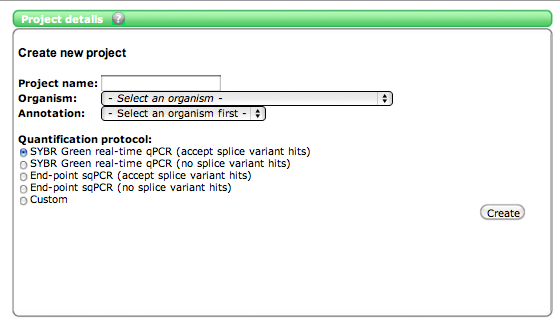
\includegraphics[width=9cm]{Figs/QP_createproject.png}
 \caption{\label{fig:QP_createproject}Creación un proyecto en {\sc Quantprime}}
\end{figure}

El siguiente paso, consiste en  incluir los transcritos para los cuales se desea diseñar primers. La Figura~\ref{fig:QP_transcripts}, muestra el formulario que nos permite completar este paso. Tiene dos opciones: i) si conoce los identificadores de los genes de interes, solo los tiene que poner en la caja de texto y presionar el botón \Verb+Add to project+, de lo contrario puede hacer búsqueda BLAST dentro de {\sc Quantprime} para encontrar los identificadores a partir de secuencias propias. En este caso vamos a diseñar primers para los genes: AT2G20825 y AT4G28190, que pertenecen a una familia pequeña de factores de transcripción conocida como ULT. Asegurese de adicionar esos identificadores a su proyecto y luego usar el botón \Verb+Select all+, seguido de \Verb+find primers+.

\begin{figure}[h!]
\centering
 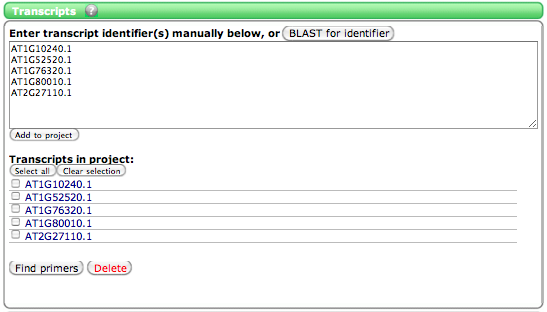
\includegraphics[width=9cm]{Figs/QP_transcripts.png}
 \caption{\label{fig:QP_transcripts}Adicionando transcritos al proyecto en  {\sc Quantprime}}
\end{figure}

En este punto se iniciará el proceso de búsqueda de primers y su posterior verificación explotando la anotación del genoma de \textit{Arabidopsis thaliana}. La Figura~\ref{fig:QP_progress} muestra la ventana de progreso de la búsqueda. Si lo desea puede cerrar esta ventana y volver as tarde a recuperar sus resultados, esta es la ventaja de estar registrado en el sitio. En la Figura~\ref{fig:QP_progress} se ve un indicador de progreso y una serie de cuatro casillas coloreadas por gen. La casilla de color verde oscuro indica el número de primers muy buenos que fueron encontrados, que cumplían con todos los criterios de búsqueda, i.e., específicos para el transcrito de interés, no amplifica ADN genómico, primers individuales no anillan con otros cDNAs. La casilla color verde claro indica el número de primers bueno, peor que podrían amplificar ADN genómico o alguno de los dos primers podría anillar con otro cDNA y por lo tanto reducir la eficiencia de la amplificación. En la casilla amarilla aparece el número de primers que se consideran adecuados, estos pueden amplificar ADN genómico, primers individuales pueden anillar a otros cDNAs. La casilla roja indica el número de primers fallidos.

La casilla verde oscura solo va a estar desactivada en aquellos casos en que la especie de interés no tenga información de su genoma en la base de datos de {\sc Quantprime}.

\begin{figure}[h!]
\centering
 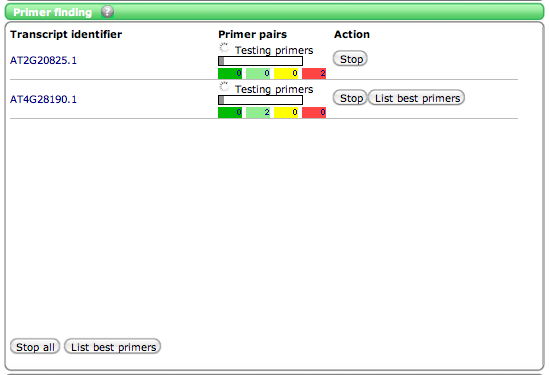
\includegraphics[width=9cm]{Figs/QP_progress.png}
 \caption{\label{fig:QP_progress}{\sc Quantprime} buscando primers para los genes solicitados}
\end{figure}

Una vez la búsqueda ha terminado , presione el botón \Verb+List best primers+ para obtener una lista detallada de los primers encontrados.

La lista de pares de primers está ordenada de acuerdo al color, como se explicó anteriormente, y en segundo lugar por el puntaje de rango de Primer3, la columna en el extremo derecho, el cual refleja la desviación de los criterios de diseño optimo y el riesgo de formar estructuras secundarias y dímeros de primers. Los mejores primers son aquellos en que este número es más pequeño.

El botón \Verb+Select best+ selecciona los mejores primers de los genes que se analizaron. 

\begin{figure}[h!]
\centering
 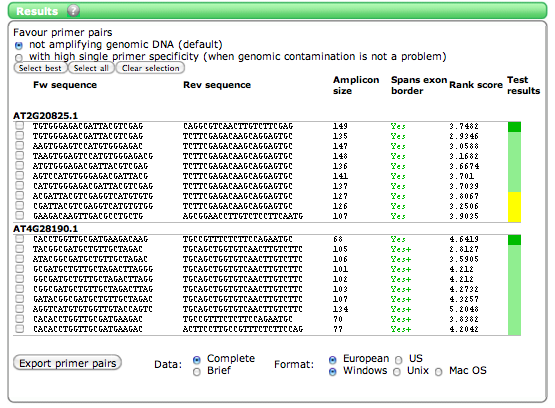
\includegraphics[width=9cm]{Figs/QP_results.png}
 \caption{\label{fig:QP_results}Listado de los mejores primers encontrados por {\sc Quantprime}}
\end{figure}

Si desea ver información mas detallada sobre cada par de primers haga clic sobre el par de interés, esto lo conducirá a la página de información de ese par de primers en particular (Figura~\ref{fig:QP_primerinfo}. En la parte superior de esta página encontrará información sobre el transcrito para el cual se diseñaron los primers.

\begin{figure}[h!]
\centering
 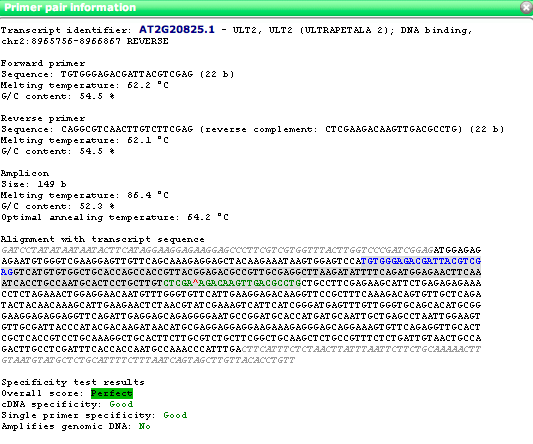
\includegraphics[width=9cm]{Figs/QP_primerinfo.png}
 \caption{\label{fig:QP_primerinfo}Página de información para un par de primers seleccionados}
\end{figure}

En la Figura~\ref{fig:QP_primerinfo}, el amplicón aparece marcado con fondo gris, primers que anillan en límites entre exones aparecen en color verde, y el limite entre los exones se indica con el símbolo \textasciicircum, los primers que aparecen en color azul no anillan sobre límites entre exones. En está página también encuentra la T$_m$ de cada primer, del amplicón y la temperatura óptima de anillamiento, asi como otras características de los primers. Al final de la página encuentra información sobre los resultados de las pruebas de especificidad que se llevaron  a cabo.

Revise la página de resultados del par de primer para un par bueno o muy bueno y para un para adecuado o malo, identifique las diferencias.

Vuelva a la página de resultados. En la parte inferior de la página encontrará el botón \Verb+Export primer pairs+, que le permite enviar los pares de primers seleccionados a un archivo de texto.

\section{Crear primers a partir de alineamientos de proteínas}

En esta sección vamos a usar el programa iCODEHOP\footnote{\url{https://icodehop.cphi.washington.edu/i-codehop-context/Welcome}} para diseñar primers a partir de un alineamiento de proteínas.

Vamos a usar el alineamiento de las 22 secuencias de primates que usó hace alguans semanas. Asegurese que el alineamiento está en formato fasta o clustal.

Siga el enlace \url{https://icodehop.cphi.washington.edu/i-codehop-context/Welcome} que lo llevará al sitio web de iCODEHOP. 

Inicie una sesión, esto lo llevará a una nueva página que luce como aparece en la Figura~\ref{fig:CODEHOP_start}, seleccione la opción \Verb+Design Primers+

\begin{figure}[h!]
\centering
 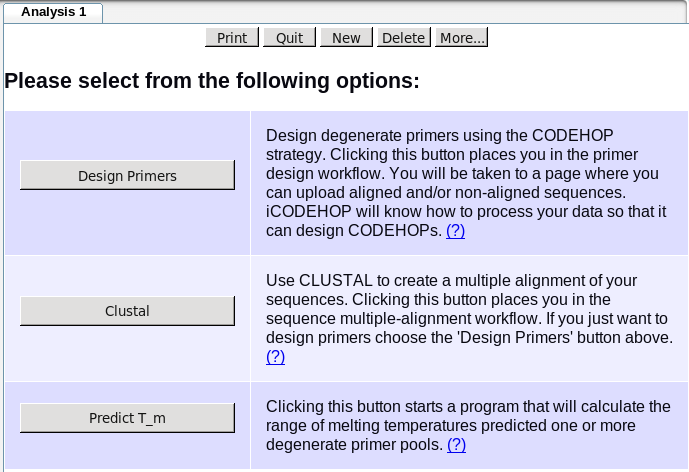
\includegraphics[width=9cm]{Figs/CODEHOP_start.png}
 \caption{\label{fig:CODEHOP_start}Página de inicio en iCODEHOP}
\end{figure}

\begin{figure}[hb!]
\centering
 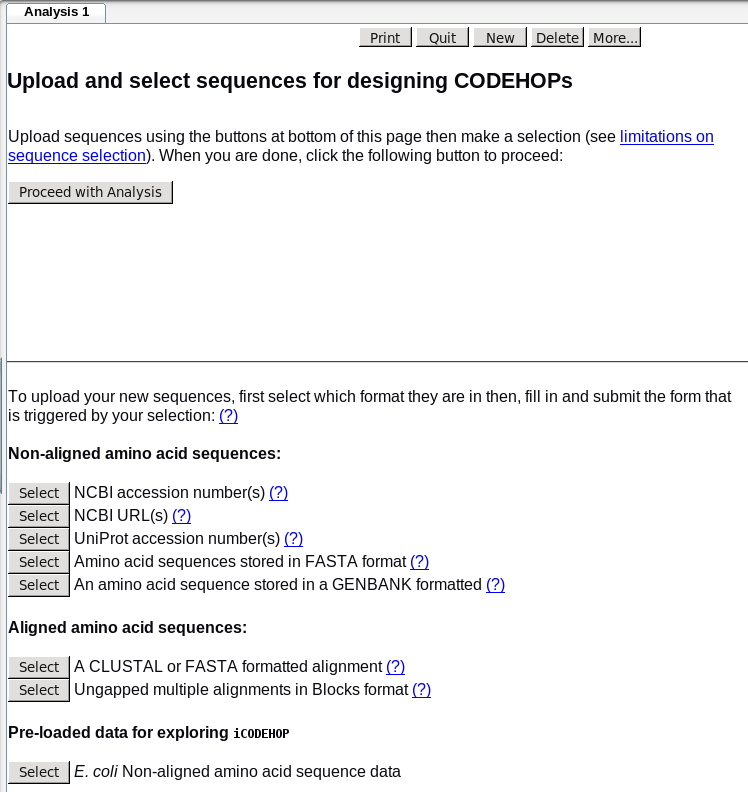
\includegraphics[width=9cm]{Figs/CODEHOP_design.png}
 \caption{\label{fig:CODEHOP_design}Diseño de primer en iCODEHOP}
\end{figure}

En la página de diseño de primers puede seleccionar diferentes fuentes de datos de alineamiento de proteínas (Figura~\ref{fig:CODEHOP_design}). En este ejercicio haga clic en el botón \Verb+Select+ que se encuentra en frente de \textbf{\Verb+A CLUSTAL or FASTA formated alignment+}, seleccione el archivo de alineamiento de 22 secuencias de primates. La nueva página aparece como la Figura~\ref{fig:CODEHOP_design2}. Ahora puede procede con el análisis haciendo clicl en el botón \Verb+Proceed with Analysis+.

\begin{figure}[h!]
\centering
 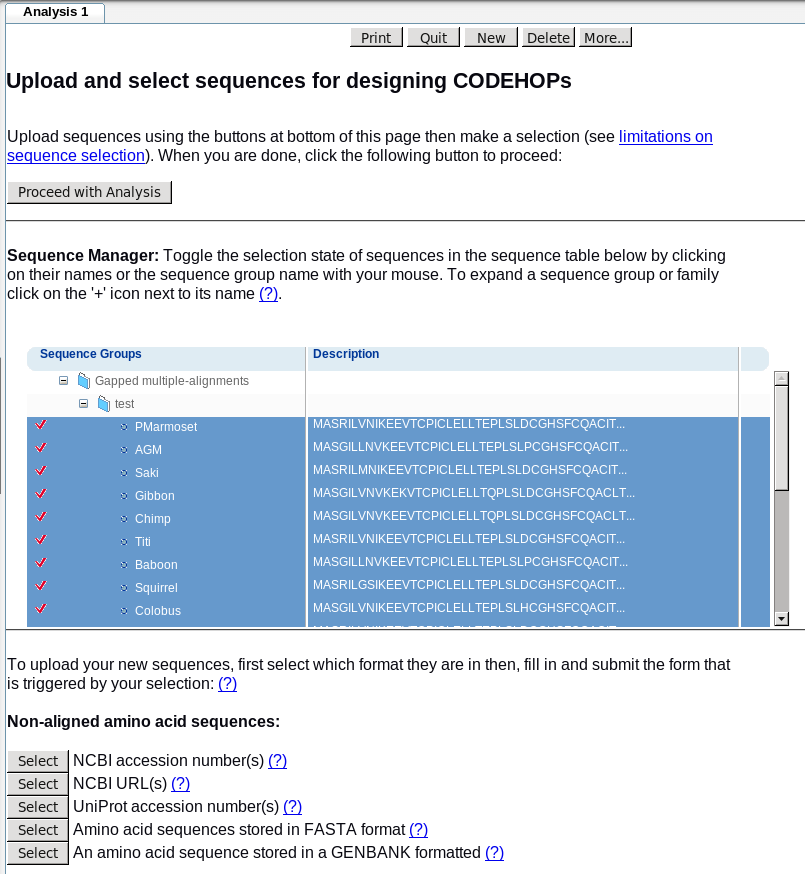
\includegraphics[width=9cm]{Figs/CODEHOP_design2.png}
 \caption{\label{fig:CODEHOP_design2}Diseño de primer en iCODEHOP}
\end{figure}

El siguiente paso en el algoritmo CODEHOP es determinar los BLOCKS\footnote{¿Qué son y como se determinan los BLOCKS?.}, esto es hecho automáticamente por iCODEHOP (figura~\ref{fig:CODEHOP_design3}). En la siguiente página selecciones el código genético y la tabal de uso de codones que serán usada en el diseño de primers. Hay otros parámetors que puede variar antes de iniciar la busqueda de primers. ¿Qué controla cada uno de esos parámetros?

\begin{figure}[h!]
\centering
 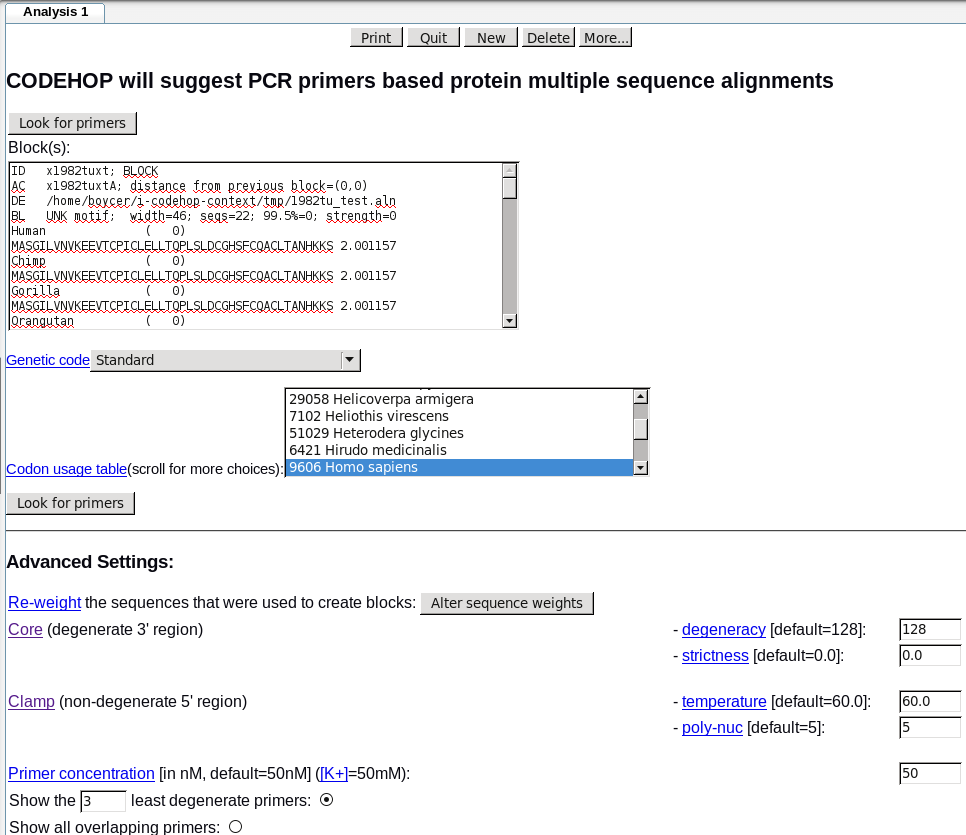
\includegraphics[width=9cm]{Figs/CODEHOP_design3.png}
 \caption{\label{fig:CODEHOP_design3}Detección de BLOCKS en el alineamineto de secuencias de proteínas. Se diseñaran primers para cada BLOCK}
\end{figure}

Uno vez esté satisfech@ con su selección de parámetros, puede dar clic en el botón \Verb+Look for primers+ para iniciar la búsqueda de primers en los BLOCKS detectados. Sea paciente la búsqueda de primers puede tomar bastante tiempo. Al finalizar la búsqueda los resultados se mostrarán en forma gráfica como aparece en la Figura~\ref{fig:CODEHOP_resultados}, al hacer clicl sobre los primers, encotrará información detallada.

Cada uno de los rectángulos que aparece en la imagen representa los BLOCKS originales, i.e., alineamientos múltiples sin gaps. El nombre del BLOCK aparece en la esquina superior izquiera del rectángulo.

Debajo del nombre del BLOCK encontrará una fila con con información sobre el número de amino ácidos que constituyen el BLOCK y la distancia en amino ácidos al BLOCK anterior y al siguiente (esto \'{u}ltimo en par\'{e}ntesis).

Enseguida encuentra el rectángulo que representa el BLOCK, aparece la secuencia consenso del alineamiento m\'{u}ltiple. El s\'{i}mbolo \textbf{*} aparece encima de los residuos completamente conservados. Amino \'{a}acidos en may\'{u}scula representan sitios altamente conservados mientras que aquellos en min\'{u}scula representan sitios con un bajo nivel de conservaci\'{o}n.

Debajo del rectángulo encuetrara los primers degenerados representados por flechas. Las flechas que se dirigen a la derecha, corresponden a los primer \textbf{forward}, las uqe se dirigen a la izquierda corresponden a los primers \textbf{reverse}. si una flecha es roja significa que iCODEHOP no pudo extender la región consenso del gancho en su longitud completa. Esto pasa cuando hay poco conservación en el extremo 5' de la región CORE degenerada de un primer.

Puede seleccionar un primer particular haciendo click sobre la flecha que lo representa y obtener información adicional usando el botón \Verb+Complete summary+ en la parte superior de la página.

En la página \Verb+Compete summary+ encuentra información detallada sobre el BLOCK que se usó para diseñar el primer seleccionado, así como ss temeratuas de anillamiento. Mas abajo encuentra una tabla con todos los primer potenciales para usar como compañeros del primer seleccionado, cada uno con infomración del nombre del BLOCK que se usó para su diseño, y sus temperaturas de anillamiento.

\begin{figure}[h!]
\centering
 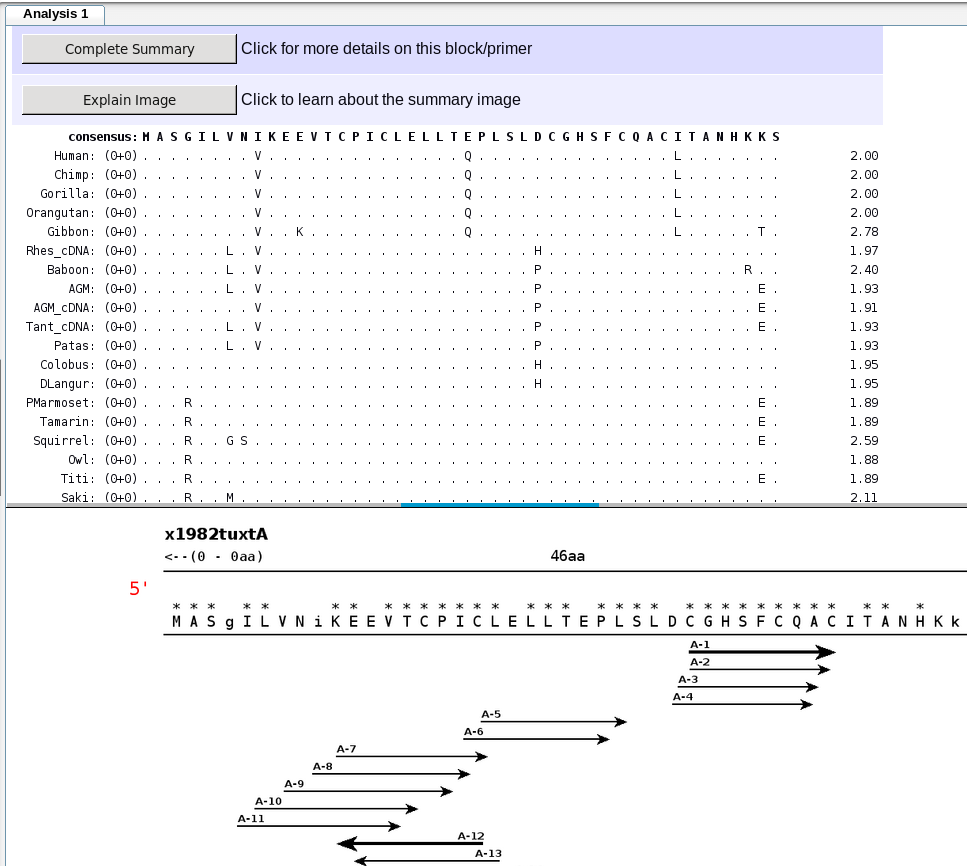
\includegraphics[width=9cm]{Figs/CODEHOP_resultados.png}
 \caption{\label{fig:CODEHOP_resultados}Detección de BLOCKS en el alineamineto de secuencias de proteínas. Se diseñaran primers para cada BLOCK}
\end{figure}
\bibliography{bibliografia}
\bibliographystyle{genetics}

\begin{appendices}

\label{unixguide}
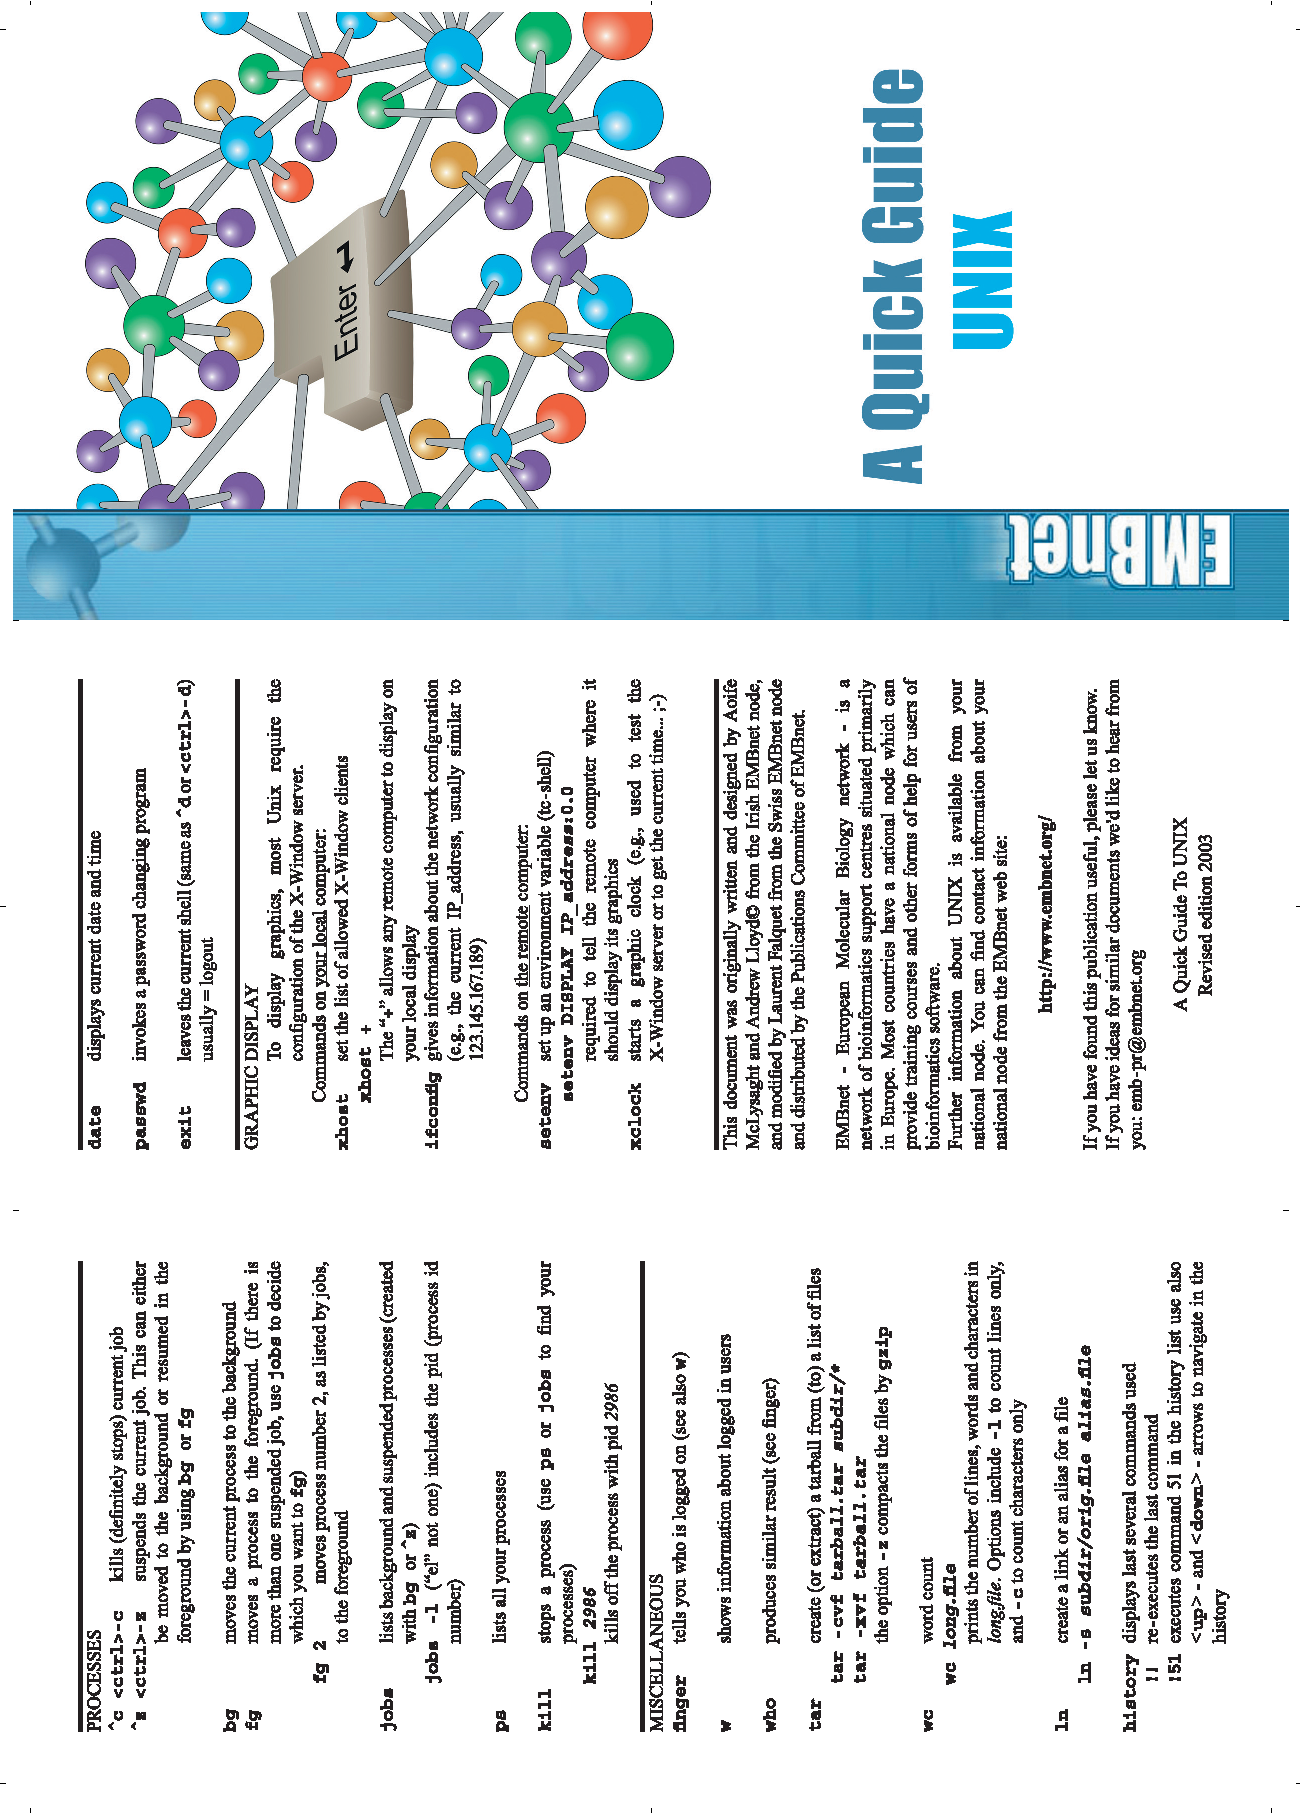
\includepdf[pages=-,fitpaper=true]{pdfs/guideUNIX.pdf}

\label{embossguide}
\includepdf[pages={2,1},fitpaper=true]{pdfs/guideEMBOSS.pdf}

\label{blastguide}
\includepdf[pages={2,1},fitpaper=true]{pdfs/guideBLAST.pdf}
\end{appendices} 

\end{document}
